\chapter{Particle Physics for the Data Analyst}\label{ch:T4}

\providecommand{\tfouraR}[2]{\num[round-mode=places,round-precision=#1]{#2}}
\providecommand{\tfouraN}[1]{\num{#1}}

\providecommand{\TfWinNom}{}\renewcommand{\TfWinNom}{75.53}
\providecommand{\TfWinResUp}{}\renewcommand{\TfWinResUp}{69.61}
\providecommand{\TfWinResDn}{}\renewcommand{\TfWinResDn}{81.82}
\providecommand{\TfWinShift}{}\renewcommand{\TfWinShift}{74.33}
\providecommand{\TfShiftGeV}{}\renewcommand{\TfShiftGeV}{0.375}
\providecommand{\TfNdecay}{}\renewcommand{\TfNdecay}{200000}
\providecommand{\TfMaxDev}{}\renewcommand{\TfMaxDev}{2.211\times10^{-11}}
\providecommand{\TfElo}{}\renewcommand{\TfElo}{36.38}
\providecommand{\TfEhi}{}\renewcommand{\TfEhi}{660.5}
\providecommand{\TfAeta}{}\renewcommand{\TfAeta}{0.6313}
\providecommand{\TfAall}{}\renewcommand{\TfAall}{0.5514}
\providecommand{\TfAerr}{}\renewcommand{\TfAerr}{0.001112}
\providecommand{\TfSigMeas}{}\renewcommand{\TfSigMeas}{1.17}
\providecommand{\TfSigPred}{}\renewcommand{\TfSigPred}{1.169}
\providecommand{\TfSigEff}{}\renewcommand{\TfSigEff}{1.154}
\providecommand{\TfRtyp}{}\renewcommand{\TfRtyp}{1.446}
\providecommand{\TfRtypM}{}\renewcommand{\TfRtypM}{1.022}
\providecommand{\TfFwBZ}{}\renewcommand{\TfFwBZ}{2.495}
\providecommand{\TfFwGZ}{}\renewcommand{\TfFwGZ}{3.532}
\providecommand{\TfFwVZ}{}\renewcommand{\TfFwVZ}{5.052}
\providecommand{\TfFwVH}{}\renewcommand{\TfFwVH}{3.77}
\providecommand{\TfFwGH}{}\renewcommand{\TfFwGH}{3.768}
\providecommand{\TfVHrel}{}\renewcommand{\TfVHrel}{0.001021}
\providecommand{\TfAcb}{}\renewcommand{\TfAcb}{133.6}
\providecommand{\TfBcb}{}\renewcommand{\TfBcb}{1.833}
\providecommand{\TfTailFrac}{}\renewcommand{\TfTailFrac}{10.37}
\providecommand{\TfFwCB}{}\renewcommand{\TfFwCB}{2.355}
\providecommand{\TfdNfiles}{}\renewcommand{\TfdNfiles}{4}
\providecommand{\TfdNtot}{}\renewcommand{\TfdNtot}{7798424}
\providecommand{\TfdNsel}{}\renewcommand{\TfdNsel}{151767}
\providecommand{\TfdPtA}{}\renewcommand{\TfdPtA}{176.1}
\providecommand{\TfdPtB}{}\renewcommand{\TfdPtB}{39.63}
\providecommand{\TfdEtaA}{}\renewcommand{\TfdEtaA}{-0.8335}
\providecommand{\TfdEtaB}{}\renewcommand{\TfdEtaB}{0.0947}
\providecommand{\TfdPhiA}{}\renewcommand{\TfdPhiA}{-0.2942}
\providecommand{\TfdPhiB}{}\renewcommand{\TfdPhiB}{0.5673}
\providecommand{\TfdEA}{}\renewcommand{\TfdEA}{240.9}
\providecommand{\TfdEB}{}\renewcommand{\TfdEB}{39.81}
\providecommand{\TfdEcalcA}{}\renewcommand{\TfdEcalcA}{240.9}
\providecommand{\TfdEcalcB}{}\renewcommand{\TfdEcalcB}{39.81}
\providecommand{\TfdMfirst}{}\renewcommand{\TfdMfirst}{106.4}
\providecommand{\TfdMvec}{}\renewcommand{\TfdMvec}{106.4}
\providecommand{\TfdNmc}{}\renewcommand{\TfdNmc}{1054711}
\providecommand{\TfdEffA}{}\renewcommand{\TfdEffA}{0.3872}
\providecommand{\TfdNexp}{}\renewcommand{\TfdNexp}{395}
\providecommand{\TfdNprod}{}\renewcommand{\TfdNprod}{1020}
\providecommand{\TfdNmcstat}{}\renewcommand{\TfdNmcstat}{0.4842}
\providecommand{\TfdXsecTree}{}\renewcommand{\TfdXsecTree}{0.102}
\providecommand{\TfdSumwTree}{}\renewcommand{\TfdSumwTree}{55922616}
\providecommand{\TfdSigMC}{}\renewcommand{\TfdSigMC}{2.398}
\providecommand{\TfdMedMC}{}\renewcommand{\TfdMedMC}{125}
\providecommand{\TfdFracTwo}{}\renewcommand{\TfdFracTwo}{93.09}
\providecommand{\TfdLowTail}{}\renewcommand{\TfdLowTail}{0.8286}
\providecommand{\TfdHighTail}{}\renewcommand{\TfdHighTail}{0.5359}
\providecommand{\TfdBwin}{}\renewcommand{\TfdBwin}{26254}
\providecommand{\TfdNwin}{}\renewcommand{\TfdNwin}{26457}
\providecommand{\TfdSwin}{}\renewcommand{\TfdSwin}{371.2}
\providecommand{\TfdSlope}{}\renewcommand{\TfdSlope}{-0.02311}
\providecommand{\TfdSoverB}{}\renewcommand{\TfdSoverB}{1.414}
\providecommand{\TfdZsimple}{}\renewcommand{\TfdZsimple}{2.291}
\providecommand{\TfdIsoData}{}\renewcommand{\TfdIsoData}{56.01}
\providecommand{\TfdIsoMC}{}\renewcommand{\TfdIsoMC}{97.68}
\providecommand{\TfdCrack}{}\renewcommand{\TfdCrack}{3.236}
\providecommand{\TfdConv}{}\renewcommand{\TfdConv}{34.66}
\providecommand{\TfdSystRel}{}\renewcommand{\TfdSystRel}{0.7112}
\providecommand{\TfdFlowDA}{}\renewcommand{\TfdFlowDA}{7798424}
\providecommand{\TfdFlowSA}{}\renewcommand{\TfdFlowSA}{543.6}
\providecommand{\TfdFlowDB}{}\renewcommand{\TfdFlowDB}{7798424}
\providecommand{\TfdFlowSB}{}\renewcommand{\TfdFlowSB}{543.6}
\providecommand{\TfdFlowDC}{}\renewcommand{\TfdFlowDC}{7798424}
\providecommand{\TfdFlowSC}{}\renewcommand{\TfdFlowSC}{543.6}
\providecommand{\TfdFlowDD}{}\renewcommand{\TfdFlowDD}{979059}
\providecommand{\TfdFlowSD}{}\renewcommand{\TfdFlowSD}{432.8}
\providecommand{\TfdFlowDE}{}\renewcommand{\TfdFlowDE}{976883}
\providecommand{\TfdFlowSE}{}\renewcommand{\TfdFlowSE}{431.9}
\providecommand{\TfdFlowDF}{}\renewcommand{\TfdFlowDF}{621499}
\providecommand{\TfdFlowSF}{}\renewcommand{\TfdFlowSF}{409.2}
\providecommand{\TfdFlowDG}{}\renewcommand{\TfdFlowDG}{397846}
\providecommand{\TfdFlowSG}{}\renewcommand{\TfdFlowSG}{395.1}
\providecommand{\TfdFlowDH}{}\renewcommand{\TfdFlowDH}{151767}
\providecommand{\TfdFlowSH}{}\renewcommand{\TfdFlowSH}{395}
\providecommand{\TflOverlapErr}{}\renewcommand{\TflOverlapErr}{3.531\times10^{-14}}
\providecommand{\TflLheadOn}{}\renewcommand{\TflLheadOn}{1.192\times10^{34}}
\providecommand{\TflLdesign}{}\renewcommand{\TflLdesign}{9.961\times10^{33}}
\providecommand{\TflPileup}{}\renewcommand{\TflPileup}{24.64}
\providecommand{\TflRateInel}{}\renewcommand{\TflRateInel}{7.780\times10^{8}}
\providecommand{\TflSigmaTrue}{}\renewcommand{\TflSigmaTrue}{23.62}
\providecommand{\TflSigmaFit}{}\renewcommand{\TflSigmaFit}{23.59}
\providecommand{\TflSigmaErr}{}\renewcommand{\TflSigmaErr}{0.03015}
\providecommand{\TflSigmaRelErr}{}\renewcommand{\TflSigmaRelErr}{0.1278}
\providecommand{\TflSigVisFit}{}\renewcommand{\TflSigVisFit}{60.04}
\providecommand{\TflSigVisTrue}{}\renewcommand{\TflSigVisTrue}{60}
\providecommand{\TflPeakRate}{}\renewcommand{\TflPeakRate}{255.5}
\providecommand{\TflNpoints}{}\renewcommand{\TflNpoints}{25}
\providecommand{\TflTpoint}{}\renewcommand{\TflTpoint}{0.2}
\providecommand{\FourBScPgvFive}{}\renewcommand{\FourBScPgvFive}{1.36\times10^{-5}}
\providecommand{\FourBScZgvFive}{}\renewcommand{\FourBScZgvFive}{4.20}
\providecommand{\FourBScPlocFive}{}\renewcommand{\FourBScPlocFive}{2.87\times10^{-7}}
\providecommand{\FourBScBtot}{}\renewcommand{\FourBScBtot}{3000}
\providecommand{\FourBScSlope}{}\renewcommand{\FourBScSlope}{30}
\providecommand{\FourBScSigM}{}\renewcommand{\FourBScSigM}{1.5}
\providecommand{\FourBScNmass}{}\renewcommand{\FourBScNmass}{201}
\providecommand{\FourBScToys}{}\renewcommand{\FourBScToys}{20000}
\providecommand{\FourBScMobs}{}\renewcommand{\FourBScMobs}{142.50}
\providecommand{\FourBScMuObs}{}\renewcommand{\FourBScMuObs}{42}
\providecommand{\FourBScQobs}{}\renewcommand{\FourBScQobs}{10.79}
\providecommand{\FourBScZloc}{}\renewcommand{\FourBScZloc}{3.28}
\providecommand{\FourBScPloc}{}\renewcommand{\FourBScPloc}{5.10\times10^{-4}}
\providecommand{\FourBScPglob}{}\renewcommand{\FourBScPglob}{0.0159}
\providecommand{\FourBScPglobErr}{}\renewcommand{\FourBScPglobErr}{0.0009}
\providecommand{\FourBScZglob}{}\renewcommand{\FourBScZglob}{2.15}
\providecommand{\FourBScTrials}{}\renewcommand{\FourBScTrials}{31.3}
\providecommand{\FourBScNzeroHundred}{}\renewcommand{\FourBScNzeroHundred}{2.78}
\providecommand{\FourBScNzeroAll}{}\renewcommand{\FourBScNzeroAll}{2.804}
\providecommand{\FourBScNone}{}\renewcommand{\FourBScNone}{3.60}
\providecommand{\FourBScPgv}{}\renewcommand{\FourBScPgv}{0.0167}
\providecommand{\FourBScFracZero}{}\renewcommand{\FourBScFracZero}{0.508}
\providecommand{\FourBScPfourMC}{}\renewcommand{\FourBScPfourMC}{0.0234}
\providecommand{\FourBScPfourTh}{}\renewcommand{\FourBScPfourTh}{0.0228}
\providecommand{\FourBScPthreeGlob}{}\renewcommand{\FourBScPthreeGlob}{0.040}
\providecommand{\FourBScTrialsThreeAsym}{}\renewcommand{\FourBScTrialsThreeAsym}{28}
\providecommand{\HyyNData}{}\renewcommand{\HyyNData}{76394}
\providecommand{\HyyNCat}{}\renewcommand{\HyyNCat}{8582}
\providecommand{\HyyNTrig}{}\renewcommand{\HyyNTrig}{7798424}
\providecommand{\HyyNTwo}{}\renewcommand{\HyyNTwo}{979404}
\providecommand{\HyyNIso}{}\renewcommand{\HyyNIso}{362972}
\providecommand{\HyyNKin}{}\renewcommand{\HyyNKin}{322243}
\providecommand{\HyyNAll}{}\renewcommand{\HyyNAll}{7798424}
\providecommand{\HyySigExp}{}\renewcommand{\HyySigExp}{397.9}
\providecommand{\HyySigCat}{}\renewcommand{\HyySigCat}{58.8}
\providecommand{\HyySigTrig}{}\renewcommand{\HyySigTrig}{610.9}
\providecommand{\HyySigTwo}{}\renewcommand{\HyySigTwo}{485.2}
\providecommand{\HyySigIso}{}\renewcommand{\HyySigIso}{430}
\providecommand{\HyySigKin}{}\renewcommand{\HyySigKin}{398.1}
\providecommand{\HyySigAll}{}\renewcommand{\HyySigAll}{610.9}
\providecommand{\HyyEffSig}{}\renewcommand{\HyyEffSig}{0.651}
\providecommand{\HyyRelSyst}{}\renewcommand{\HyyRelSyst}{0.0086}
\providecommand{\HyyNA}{}\renewcommand{\HyyNA}{4227}
\providecommand{\HyyNB}{}\renewcommand{\HyyNB}{14804}
\providecommand{\HyyNC}{}\renewcommand{\HyyNC}{21876}
\providecommand{\HyyND}{}\renewcommand{\HyyND}{35487}
\providecommand{\HyySigggH}{}\renewcommand{\HyySigggH}{357.2}
\providecommand{\HyySigVBF}{}\renewcommand{\HyySigVBF}{29.9}
\providecommand{\HyySigWH}{}\renewcommand{\HyySigWH}{5.6}
\providecommand{\HyySigZH}{}\renewcommand{\HyySigZH}{5.3}
 
\section*{Where this chapter is going}
\addcontentsline{toc}{section}{Where this chapter is going}
\label{T4a:sec:roadmap}

Two beams of protons circle the Large Hadron Collider in opposite directions and cross each other forty million times a second. At every crossing a few dozen pairs of protons collide. Almost all of these collisions are ordinary: the protons break up into sprays of light particles that the theory has described for decades. Roughly once in a billion and a half collisions something rarer happens, and a Higgs boson is made. It lives for about $10^{-22}$\,s, far too short to travel a measurable distance, and in about two decays out of a thousand it turns into two photons. The detector never sees the Higgs boson. It sees two photons, measures their energies and their directions, and writes these numbers to disk together with everything else that happened in that crossing.

From the two photons of an event one number can be computed that does not care how fast the Higgs boson was moving: the \emph{invariant mass} of the pair. For a Higgs decay it is always $125$\,GeV, up to the blurring of the measurement. For the many ordinary events that also contain two photons it is spread over a smooth, falling range. So a histogram of this one number, made from millions of events, shows a smooth background with a small bump on it. That histogram is the data of the Higgs discovery of 2012, and of the capstone of \cref{ch:13}, where we analyse the real collision data that the ATLAS experiment has released to the public.

The statistics of the search, worked out in \cref{ch:04}, needs one thing from physics: the \emph{expected} number of events in each bin of that histogram, as a function of a few parameters. Each piece of that expectation is a physical quantity. How often the process happens is a cross section $\sigma$. How many collisions were recorded is the integrated luminosity $L$. What fraction of the produced events the detector keeps are the acceptance $A$ and the efficiency $\varepsilon$. Where the kept events land on the mass axis is a template, made by simulating the detector. How much of the predicted signal is really there is the signal strength $\mu$. How well all of these are known is described by a handful of nuisance parameters $\bm\theta$, each pinned down by a calibration. \Cref{T4a:fig:roadmap} shows how they connect.

\begin{figure}[htbp]
\centering
\begin{tikzpicture}[
  box/.style={draw=accent,rounded corners=2pt,fill=ideabg,align=center,font=\small,
              minimum width=2.9cm,minimum height=1.05cm,inner sep=3pt},
  phys/.style={box,draw=formblue},
  det/.style={box,fill=warnbg,draw=bdryred},
  stat/.style={box,fill=takebg,draw=tangentgreen},
  arr/.style={->,thick,accent}]
  \node[phys] (coll) at (0,0) {collisions\\ $\sigma$, $L$, $N=\sigma L$\\ \S\ref{T4a:sec:events}, \S\ref{T4a:sec:xsec}};
  \node[det] (obj) at (4.3,0) {recorded objects\\ $p_T,\ \eta,\ \phi,\ E$\\ \S\ref{T4a:sec:events}};
  \node[det] (sel) at (8.6,0) {selection\\ acceptance $A$,\\ efficiency $\varepsilon$};
  \node[phys] (mass) at (8.6,-2.3) {invariant mass $m$\\ peak and width\\ \S\ref{T4a:sec:mass}};
  \node[phys] (tmpl) at (4.3,-2.3) {templates $s_i$, $b_i$\\ signal strength $\mu$\\ \S\ref{T4a:sec:templates}};
  \node[det] (nuis) at (0,-2.3) {calibrations\\ nuisance $\bm\theta$\\ \S\ref{T4a:sec:nuisance}};
  \node[stat] (nu) at (4.3,-4.6) {expected counts\\ $\nu_i(\mu,\bm\theta)=\mu s_i(\bm\theta)+b_i(\bm\theta)$};
  \node[stat] (stat) at (8.6,-4.6) {likelihood, $q_0$, CL$_s$\\ Ch.~\ref{ch:04};\ data: Ch.~\ref{ch:13}};
  \node[box] (higgs) at (0,-4.6) {the 2012 Higgs search\\ \S\ref{T4a:sec:higgs};\ open data \S\ref{T4a:sec:opendata}};
  \draw[arr] (coll) -- (obj);
  \draw[arr] (obj) -- (sel);
  \draw[arr] (sel) -- (mass);
  \draw[arr] (mass) -- (tmpl);
  \draw[arr] (nuis) -- (tmpl);
  \draw[arr] (tmpl) -- (nu);
  \draw[arr] (nu) -- (stat);
  \draw[arr,dashed] (higgs) -- (nu);
\end{tikzpicture}
\caption{The path from collisions to the numbers the statistics uses. Blue boxes are physics that theory and simulation predict: how often a process happens, and where its events land on the mass axis. Red boxes are what the detector and the analysis do to the events: record them, keep some of them, and get calibrated. The two green boxes are where the statistics of \cref{ch:04} takes over: every arrow above ends in the expected count $\nu_i$ of one histogram bin, and the likelihood compares those expectations with the observed counts.}
\label{T4a:fig:roadmap}
\end{figure}

A collider produces collisions at a known rate, and the expected number of events of any kind is its cross section times the integrated luminosity, $N=\sigma L$; the formula follows from the overlap of two bunches of protons, and the number actually recorded is a Poisson count (\cref{T4a:sec:xsec}). What is counted is a recorded event: a list of reconstructed particles, each with a transverse momentum $p_T$, a pseudorapidity $\eta$ and an azimuth $\phi$ (\cref{T4a:sec:events}). From two of these particles comes the invariant mass, which is the same in every decay of a given particle; its spread comes from the lifetime of the particle and from the resolution of the detector, and both shapes can be derived (\cref{T4a:sec:mass}). Simulated events and the side regions of the data give the expected shapes of signal and background, the templates, and the signal strength $\mu$ scales the predicted signal (\cref{T4a:sec:templates}). Every input is known only to some precision; each imprecision becomes a nuisance parameter with its own calibration measurement (\cref{T4a:sec:nuisance}). All of these were at work in the two searches that found the Higgs boson in 2012 (\cref{T4a:sec:higgs}), and every one has a column, or a combination of columns, in the open-data files that \cref{ch:13} analyses (\cref{T4a:sec:opendata}). \Cref{T4a:tab:symbols} lists each symbol with its typical size and the place in the book where it is used.

The likelihood of a histogram, the treatment of nuisance parameters, the discovery statistic $q_0$, the look-elsewhere effect and the CL$_s$ limits are built on these expected counts in \cref{ch:04} (\cref{4b:sec:templates,4b:sec:limits,4b:sec:lee}); undoing the detector's blurring is \cref{6b:sec:unfolding}. In the language of the book's pipeline (\cref{ch:00}), the collider case reads as follows. The physical model is the Standard Model with or without the Higgs signal. The data set is the list of recorded events. What matters in it is the invariant mass of the photon pair, and the summary is a histogram of that mass. The sampling distribution of each bin is Poisson, with a mean that physics supplies. Inference then asks the question of \cref{ch:05} in its collider form: which signal strengths, and which values of the calibration constants, could have produced the histogram we recorded?
\section{What a collider does, and what an event is}
\label{T4a:sec:events}

A proton is not a hard ball. It is a bound state of quarks and gluons, together called \newterm{partons}, which share its momentum among themselves in a way that changes from one moment to the next. When two bunches of protons cross at the LHC, most protons pass each other untouched. A few pairs come close enough for one parton of each to collide hard. Those two partons, not the whole protons, make the interesting new particles. Each parton carries an unknown fraction of its proton's momentum, so the collision we care about happens in a frame that moves along the beam line at a speed we do not know. Everything else in the two protons sprays out as low-energy debris, mostly close to the beam.

Around the collision point sits the detector, a set of nested cylinders, each built to measure one kind of particle. A crossing of two bunches lasts a fraction of a nanosecond, and the next one comes 25\,ns later. Only a few hundred crossings per second can be written to disk, so fast electronics, the \newterm{trigger}, decide within microseconds whether a crossing looks interesting enough to keep, for example because two large deposits of electromagnetic energy appeared in the calorimeter \cite{ATLASDetector2008}. What is kept is the raw response of millions of detector channels. Reconstruction programs then turn these responses into a short list of particles with measured momenta. That list is what an analyst works with.

\paragraph{The questions in words.}
\begin{enumerate}[label=\arabic*.]
  \item What does the detector record, and how does a photon look different from an electron, a muon, a jet or a neutrino?
  \item Which numbers describe a recorded particle, and why does a hadron collider describe directions by a pseudorapidity $\eta$ instead of the polar angle $\theta$?
  \item What is the energy of a photon in terms of those numbers?
\end{enumerate}

\subsection{The detector, layer by layer}
\label{T4a:sec:detector}

The ATLAS detector used for the Higgs search has four layers \cite[Sec.~2]{AadHiggs2012}, \cite{ATLASDetector2008}. Going outwards from the beam:
\begin{itemize}[itemsep=1pt,leftmargin=1.2em]
  \item The \newterm{inner detector}: layers of silicon sensors and straw tubes inside a $2$\,T magnetic field. A charged particle leaves a trail of hits, and the curvature of the trail in the field gives its momentum. Neutral particles leave nothing here.
  \item The \newterm{electromagnetic calorimeter}: liquid argon between lead plates. Photons and electrons dump all their energy in it, in a narrow shower. Its first layer is finely segmented in angle, so that a single photon can be told apart from the two nearby photons of a decaying neutral pion.
  \item The \newterm{hadronic calorimeter}: iron and scintillating tiles. Protons, pions and the other strongly interacting particles shower here.
  \item The \newterm{muon spectrometer}: tracking chambers in a toroidal magnetic field outside everything else. Muons are the only charged particles that cross the calorimeters.
\end{itemize}
Each kind of particle leaves a different pattern across the layers, and the pattern is its identity. \Cref{T4a:fig:detector} draws the five patterns that matter.

\begin{figure}[htbp]
\centering
\begin{tikzpicture}[scale=1.0]
  \def\rid{1.4}\def\rem{2.3}\def\rhad{3.3}\def\rmu{4.4}
  \fill[formblue!8] (0,0) -- (\rid,0) arc (0:90:\rid) -- cycle;
  \fill[fibreorange!12] (\rid,0) arc (0:90:\rid) -- (0,\rem) arc (90:0:\rem) -- cycle;
  \fill[bdryred!8] (\rem,0) arc (0:90:\rem) -- (0,\rhad) arc (90:0:\rhad) -- cycle;
  \fill[tangentgreen!8] (\rhad,0) arc (0:90:\rhad) -- (0,\rmu) arc (90:0:\rmu) -- cycle;
  \foreach \r in {\rid,\rem,\rhad,\rmu} \draw[faint] (\r,0) arc (0:90:\r);
  \draw[faint] (0,0) -- (\rmu,0); \draw[faint] (0,0) -- (0,\rmu);
  \node[lbl,align=center,anchor=north] at (0.75,-0.05) {\scriptsize inner\\[-2pt]\scriptsize detector};
  \node[lbl,align=center,anchor=north] at (1.85,-0.05) {\scriptsize EM\\[-2pt]\scriptsize calo};
  \node[lbl,align=center,anchor=north] at (2.8,-0.05) {\scriptsize hadronic\\[-2pt]\scriptsize calo};
  \node[lbl,align=center,anchor=north] at (3.85,-0.05) {\scriptsize muon\\[-2pt]\scriptsize chambers};
  \draw[dashed,thick,fibreorange] (0,0) -- (80:\rid);
  \fill[fibreorange] (80:1.95) ellipse [x radius=0.09,y radius=0.3,rotate=-10];
  \node[lbl,anchor=south] at (80:\rmu+0.05) {$\gamma$};
  \draw[faint,densely dotted] (80:2.25) -- (80:\rmu);
  \draw[thick,formblue] (0,0) to[bend left=6] (65:\rid);
  \fill[formblue] (65:1.95) ellipse [x radius=0.09,y radius=0.3,rotate=-25];
  \draw[faint,densely dotted] (65:2.25) -- (65:\rmu);
  \node[lbl,anchor=south west] at (65:\rmu) {$e$};
  \draw[thick,tangentgreen] (0,0) to[bend right=4] (48:\rmu);
  \node[lbl,anchor=south west] at (48:\rmu) {$\mu$};
  \foreach \a in {27,30,33} \draw[thin,bdryred] (0,0) -- (\a:\rid);
  \fill[bdryred!70] (30:1.95) ellipse [x radius=0.12,y radius=0.32,rotate=-60];
  \fill[bdryred] (30:2.8) ellipse [x radius=0.2,y radius=0.45,rotate=-60];
  \draw[faint,densely dotted] (30:3.25) -- (30:\rmu);
  \node[lbl,anchor=west] at (30:\rmu) {jet};
  \draw[softgray,densely dotted,thick] (0,0) -- (12:\rmu);
  \node[lbl,anchor=west] at (12:\rmu) {$\nu$: nothing};
  \fill (0,0) circle (1.5pt);
\end{tikzpicture}
\caption{A quarter of the detector seen along the beam, with the beam at the lower left corner, and the five signatures. A photon leaves no track and a narrow shower in the electromagnetic calorimeter. An electron leaves a track and the same narrow shower. A muon crosses everything. A jet, the spray of hadrons from a quark or gluon, leaves several tracks and showers in both calorimeters. A neutrino leaves nothing at all; it shows up only as an imbalance of the momenta of everything else.}
\label{T4a:fig:detector}
\end{figure}

\begin{workdef}[event and reconstructed object]
An \newterm{event} is everything recorded in one bunch crossing that the trigger kept. A \newterm{reconstructed object} is one particle candidate built from it, a photon, electron, muon, jet or hadronic tau decay, with four measured numbers: its transverse momentum $p_T$, pseudorapidity $\eta$, azimuth $\phi$ and energy $E$, plus quality flags. \emph{Operationally:} an event in the files of \cref{T4a:sec:opendata} is one row of a table; each kind of object fills a set of columns that hold one entry per object of that kind \unpack{a row with three photons has three numbers in the photon-$p_T$ column}.
\end{workdef}

Two of the identity rules need a word more. A photon can convert into an electron--positron pair in the material in front of the calorimeter; it then leaves one or two tracks that start in the middle of the inner detector instead of at the collision point, and is recognised as a \emph{converted} photon. In the open data, about a third of the selected photons are converted ($\TfdConv\%$). And a jet is not one particle but the collimated spray of hadrons that a quark or gluon becomes; its energy is the sum of everything in a cone around its axis.

\subsection{Coordinates: why the transverse plane}
\label{T4a:sec:coordinates}

ATLAS uses a right-handed frame with the origin at the collision point and the $z$ axis along the beam \cite[footnote 2]{AadHiggs2012}. The polar angle $\theta$ is measured from the $z$ axis, and the azimuth $\phi$ around it, in the plane perpendicular to the beam called the \newterm{transverse plane}. A particle's momentum splits into a part along the beam, $p_z=\lvert\bm p\rvert\cos\theta$, and a part in the transverse plane, of size
\begin{equation}
  p_T=\sqrt{p_x^2+p_y^2}=\lvert\bm p\rvert\sin\theta .
  \label{T4a:eq:pt}
\end{equation}

\emph{Why the transverse part is special.} Before the collision, the two partons move along the beam. Their momenta along $z$ are $x_1E_{\rm b}$ and $-x_2E_{\rm b}$, where $E_{\rm b}$ is the beam energy and $x_1,x_2$ are the momentum fractions the two partons happened to carry. Neither fraction is measured, so the total $z$ momentum of the hard collision, $(x_1-x_2)E_{\rm b}$, is unknown in every event. Their transverse momenta, on the other hand, are close to zero. Momentum conservation then says that the transverse momenta of everything produced add up to zero, while it says nothing useful about the $z$ momenta. Two consequences follow. A particle that escapes unseen, like a neutrino, shows up as an imbalance of the transverse momenta of the visible particles, the \newterm{missing transverse momentum} $-\sum_i\bm p_{T,i}$ \cite[(49.49)]{PDG2024}; and the description of a particle should use quantities that do not change when the whole event is boosted along $z$ by an unknown amount.

\emph{A variable that adds under boosts.} The \newterm{rapidity} of a particle is \cite[(49.40)]{PDG2024}
\begin{equation}
  y=\frac12\ln\frac{E+p_z}{E-p_z}.
  \label{T4a:eq:rapidity}
\end{equation}
What happens to it under a boost along $z$ with velocity $\beta$ (in units of $c=1$) and $\gamma=(1-\beta^2)^{-1/2}$? The Lorentz transformation of \cite[(49.1)]{PDG2024} gives $E'=\gamma(E-\beta p_z)$ and $p_z'=\gamma(p_z-\beta E)$. Then
\begin{align}
  y'&\eqby{1}\frac12\ln\frac{\gamma(E-\beta p_z)+\gamma(p_z-\beta E)}{\gamma(E-\beta p_z)-\gamma(p_z-\beta E)}
     \eqby{2}\frac12\ln\frac{(1-\beta)(E+p_z)}{(1+\beta)(E-p_z)}\nonumber\\
    &\eqby{3}y+\frac12\ln\frac{1-\beta}{1+\beta}
     \eqby{4}y-\tanh^{-1}\beta .
  \label{T4a:eq:y-boost}
\end{align}
\begin{explain}
  \item Insert the boosted energy and momentum into \eqref{T4a:eq:rapidity}.
  \item Collect terms: the numerator is $\gamma(E+p_z)(1-\beta)$ and the denominator $\gamma(E-p_z)(1+\beta)$; the $\gamma$'s cancel.
  \item The logarithm of a product is the sum of the logarithms.
  \item $\tanh^{-1}\beta=\frac12\ln\frac{1+\beta}{1-\beta}$, the inverse of $\tanh u=(e^{u}-e^{-u})/(e^{u}+e^{-u})$.
\end{explain}
A boost along the beam shifts every rapidity in the event by the same amount. The \emph{difference} of two rapidities is therefore the same in every frame, and so is the shape of a distribution of rapidities \cite[\S49.5.2]{PDG2024}. The unknown motion of the parton pair along the beam drops out of every rapidity difference.

\emph{From rapidity to an angle.} Rapidity needs the energy and $p_z$, and so the mass. For a massless particle, or any particle with $\lvert\bm p\rvert\gg m$, $E=\lvert\bm p\rvert$ and $p_z=\lvert\bm p\rvert\cos\theta$, and the rapidity becomes a function of the angle alone:
\begin{align}
  y&\eqby{1}\frac12\ln\frac{1+\cos\theta}{1-\cos\theta}
    \eqby{2}\frac12\ln\frac{2\cos^2(\theta/2)}{2\sin^2(\theta/2)}
    \eqby{3}-\ln\tan\frac\theta2\;\equiv\;\eta .
  \label{T4a:eq:eta}
\end{align}
\begin{explain}
  \item Divide numerator and denominator of \eqref{T4a:eq:rapidity} by $\lvert\bm p\rvert=E$.
  \item The half-angle identities $1+\cos\theta=2\cos^2(\theta/2)$ and $1-\cos\theta=2\sin^2(\theta/2)$.
  \item $\frac12\ln(\cot^2u)=\ln\cot u=-\ln\tan u$.
\end{explain}
This is the \newterm{pseudorapidity} \cite[(49.47)]{PDG2024}. It is defined for every particle as $-\ln\tan(\theta/2)$, whatever its mass, because the angle is always measured; for photons it is exactly the rapidity, and for light particles at high momentum it is very nearly so.

\begin{workdef}[pseudorapidity]
The \newterm{pseudorapidity} of a particle at polar angle $\theta$ from the beam is $\eta=-\ln\tan(\theta/2)$, and inversely $\theta=2\arctan e^{-\eta}$. It is $0$ perpendicular to the beam and grows without bound towards the beam. \emph{Operationally:} $\eta=\sinh^{-1}(p_z/p_T)$ from the measured momentum components \unpack{a form that follows from $\sinh\eta=\cot\theta$, derived below}. For a massless particle, differences of $\eta$ do not change under boosts along the beam.
\end{workdef}

\emph{Energy and momentum from $(p_T,\eta,\phi)$.} Write $t=\tan(\theta/2)$, so $e^{\eta}=1/t$ by \eqref{T4a:eq:eta}. Then
\begin{align}
  \sinh\eta&\eqby{1}\frac12\Bigl(\frac1t-t\Bigr)\eqby{2}\frac{1-t^2}{2t}\eqby{3}\cot\theta,
  &\cosh\eta&\eqby{1}\frac12\Bigl(\frac1t+t\Bigr)\eqby{2}\frac{1+t^2}{2t}\eqby{3}\frac1{\sin\theta}.
  \label{T4a:eq:eta-identities}
\end{align}
\begin{explain}
  \item The definitions $\sinh\eta=(e^\eta-e^{-\eta})/2$ and $\cosh\eta=(e^\eta+e^{-\eta})/2$, with $e^{\eta}=1/t$.
  \item Put both terms over the common denominator $2t$.
  \item The double-angle formulas in terms of $t=\tan(\theta/2)$: $\tan\theta=2t/(1-t^2)$ and $\sin\theta=2t/(1+t^2)$.
\end{explain}
Combining these with \eqref{T4a:eq:pt}, a particle's momentum components and, for a massless particle, its energy are
\begin{equation}
  p_x=p_T\cos\phi,\qquad p_y=p_T\sin\phi,\qquad p_z=p_T\sinh\eta,\qquad
  E=\lvert\bm p\rvert=\frac{p_T}{\sin\theta}=p_T\cosh\eta .
  \label{T4a:eq:four-vector}
\end{equation}
The first two are the definition of the azimuth; the third is $p_z=\lvert\bm p\rvert\cos\theta=p_T\cot\theta$ with $\cot\theta=\sinh\eta$; the last uses $\cosh\eta=1/\sin\theta$. These four numbers are all that the invariant mass of \cref{T4a:sec:mass} needs.

\paragraph{Example: angles and pseudorapidities.}
At $\theta=90^\circ$, $\tan45^\circ=1$ and $\eta=0$. At $\theta=45^\circ$, $\tan22.5^\circ=0.4142$ and $\eta=-\ln0.4142=0.881$. At $\theta=10^\circ$, $\tan5^\circ=0.08749$ and $\eta=2.436$. The pseudorapidity grows slowly over most of the detector and fast near the beam: the last $10^\circ$ next to the beam cover more than $\eta=2.4$ onwards. Going the other way, the ATLAS photon acceptance ends at $\lvert\eta\rvert=2.37$, which is $\theta=2\arctan e^{-2.37}=2\arctan0.0935=10.7^\circ$ from the beam, and the gap between the barrel and the end-cap calorimeters, $1.37<\lvert\eta\rvert<1.52$, is the thin cone between $\theta=24.7^\circ$ and $28.5^\circ$ (on each side), where cables and services pass and photons are poorly measured \cite[Sec.~5.1]{AadHiggs2012}. \Cref{T4a:fig:eta} draws these directions.

\begin{figure}[htbp]
\centering
\begin{tikzpicture}[scale=1.0]
  \draw[->,thick] (-5.4,0) -- (5.6,0) node[anchor=west,font=\small] {$z$ (beam)};
  \draw[faint] (-5,0) rectangle (5,3.2);
  \foreach \e in {0,0.5,1,2,3} {
    \pgfmathsetmacro{\th}{2*atan(exp(-\e))}
    \pgfmathsetmacro{\L}{min(3.2/sin(\th),5/max(abs(cos(\th)),0.001))}
    \draw[formblue] (0,0) -- (\th:\L);
    \draw[formblue] (0,0) -- (180-\th:\L);
  }
  \foreach \e in {0,0.5,1} {
    \pgfmathsetmacro{\th}{2*atan(exp(-\e))}
    \node[font=\scriptsize,formblue,anchor=south] at (\th:{3.2/sin(\th)}) {$\eta=\e$};
  }
  \foreach \e in {2,3} {
    \pgfmathsetmacro{\th}{2*atan(exp(-\e))}
    \node[font=\scriptsize,formblue,anchor=west] at (5,{5*tan(\th)}) {$\eta=\e$};
  }
  \foreach \e in {1.37,1.52} {
    \pgfmathsetmacro{\th}{2*atan(exp(-\e))}
    \pgfmathsetmacro{\L}{min(3.2/sin(\th),5/max(abs(cos(\th)),0.001))}
    \draw[bdryred,thick] (0,0) -- (\th:\L);
    \draw[bdryred,thick] (0,0) -- (180-\th:\L);
  }
  \pgfmathsetmacro{\thA}{2*atan(exp(-1.37))}\pgfmathsetmacro{\thB}{2*atan(exp(-1.52))}
  \fill[bdryred!15] (0,0) -- (\thB:5.4) arc (\thB:\thA:5.4) -- cycle;
  \fill[bdryred!15] (0,0) -- (180-\thA:5.4) arc (180-\thA:180-\thB:5.4) -- cycle;
  \pgfmathsetmacro{\thE}{2*atan(exp(-2.37))}
  \draw[tangentgreen,thick,dashed] (0,0) -- (\thE:5.08);
  \draw[tangentgreen,thick,dashed] (0,0) -- (180-\thE:5.08);
  \node[font=\scriptsize,bdryred,anchor=west] at (5.0,2.5) {crack};
  \node[font=\scriptsize,tangentgreen,anchor=west] at (5.0,{5*tan(\thE)}) {$\lvert\eta\rvert=2.37$};
  \fill (0,0) circle (1.6pt);
  \draw (0,0) ++(0:0.7) arc (0:{2*atan(exp(-1))}:0.7);
  \node[font=\scriptsize,anchor=west] at (25:0.75) {$\theta$};
\end{tikzpicture}
\caption{Directions of constant pseudorapidity in the plane containing the beam, drawn at their true angles $\theta=2\arctan e^{-\eta}$. Equal steps in $\eta$ crowd towards the beam. The shaded red wedges are the barrel/end-cap gap $1.37<\lvert\eta\rvert<1.52$, and the green dashed lines mark the edge $\lvert\eta\rvert=2.37$ of the region where photons are accepted.}
\label{T4a:fig:eta}
\end{figure}

\paragraph{Example: a photon's energy from its three numbers.}
A photon is recorded with $p_T=50$\,GeV and $\eta=1.2$. Then $\sinh1.2=1.5095$ and $\cosh1.2=1.8107$, so by \eqref{T4a:eq:four-vector} $p_z=75.5$\,GeV and $E=90.5$\,GeV. As a check, $p_T^2+p_z^2=2500+5697=8197\,\mathrm{GeV}^2=E^2$, as it must be for a massless particle. A photon going straight up, at $\eta=0$, would have $E=p_T$; the same $p_T$ further forward carries more energy, because most of its momentum then points along the beam.

\paragraph{Example: why the beam direction is lost.}
Suppose the two partons carry $x_1=0.02$ and $x_2=0.005$ of their protons' momenta at $E_{\rm b}=6.5$\,TeV. The parton pair then has energy $(x_1+x_2)E_{\rm b}=162.5$\,GeV and momentum $(x_1-x_2)E_{\rm b}=97.5$\,GeV along $+z$, so it moves with $\beta=97.5/162.5=0.6$ and every particle it makes has its rapidity shifted by $\tanh^{-1}0.6=\tfrac12\ln4=0.693$, by \eqref{T4a:eq:y-boost} read backwards. In the next event the fractions are different and so is the shift. A search that looked at $\eta$ itself would see the decay products smeared by this random shift; one that looks at $p_T$, at differences of $\eta$, or at the invariant mass, does not. The collision energy available to make new particles is $\sqrt{x_1x_2}\,\sqrt s=\sqrt{10^{-4}}\times13$\,TeV$=130$\,GeV in this example, which is why a $125$\,GeV Higgs boson needs only a small slice of the $13$\,TeV of the protons.

\begin{pitfall}[Pseudorapidity is an angle, rapidity is a boost]
Only rapidity differences are exactly unchanged by a boost along the beam. For a massive particle, such as a heavy jet or a slow proton, $\eta$ and $y$ differ, and $\eta$ differences do change under the boost. For photons and electrons at the energies of this chapter the two are equal to better than one part in $10^{6}$, and the distinction never matters.
\end{pitfall}

\paragraph{Where this is used.}
The photon columns of the open data (\cref{T4a:sec:opendata}) are exactly $p_T$, $\eta$, $\phi$ and $E$. The acceptance cuts $\lvert\eta\rvert<2.37$ outside $1.37$--$1.52$ appear in every diphoton selection of the book, from the toy of \cref{T4a:sec:xsec} to the capstone of \cref{ch:13}. The identity $E=p_T\cosh\eta$ is checked on a real event in \cref{T4a:sec:opendata}.
\section{Cross section, luminosity and the expected number of events}
\label{T4a:sec:xsec}

Before a search can ask whether the Higgs boson is in the data, it has to say how many Higgs bosons the data \emph{should} contain if the Standard Model is right. That prediction has two factors that come from two different communities. Theorists compute how likely the process is when two protons collide, a number with the dimension of an area called the cross section. The accelerator physicists know how many chances the beams gave for that process to happen, a number with the dimension of an inverse area called the integrated luminosity. Their product is a pure number of events. A third factor comes from the experiment itself: of the events produced, only some land in the detector where photons can be measured, and only some of those survive the selection.

\paragraph{The questions in words.}
\begin{enumerate}[label=\arabic*.]
  \item What is a cross section, as a physical picture we could draw?
  \item How many collisions do two crossing bunches of protons give, and how does that turn into the luminosity?
  \item Of the events produced, what fraction is kept, and why is the number kept a Poisson count with mean $\sigma L\varepsilon A$?
\end{enumerate}

\subsection{A cross section is an area}
\label{T4a:sec:area}

Shoot one small projectile through a thin slab of material of thickness $\dd x$ containing $n$ target particles per unit volume. Suppose each target behaves like a small disc of area $\sigma$ facing the projectile: if the projectile's path crosses the disc, the reaction happens; otherwise nothing happens. \emph{What is the probability of a reaction?} Look at a patch of the slab of area $S$ as seen by the projectile. It holds $nS\,\dd x$ targets, whose discs cover the area $nS\,\dd x\,\sigma$, and for a thin enough slab the discs do not overlap. The projectile arrives at a random point of the patch, so the probability that it hits a disc is the covered fraction,
\begin{equation}
  \Prob(\text{reaction in }\dd x)=\frac{nS\,\dd x\,\sigma}{S}=n\sigma\,\dd x .
  \label{T4a:eq:thin-target}
\end{equation}
This is the operational meaning of the \newterm{cross section} $\sigma$: the effective area a target presents for one particular reaction. It has nothing to do with the geometric size of the proton. A process with a small quantum-mechanical amplitude has a small $\sigma$, even though the protons are the same. The unit is the \newterm{barn}, $1\,\mathrm{b}=10^{-24}\,\mathrm{cm}^2$, with $1\,\mathrm{mb}=10^{-3}$\,b, $1\,\mathrm{pb}=10^{-12}$\,b and $1\,\mathrm{fb}=10^{-15}$\,b. In natural units, $(\hbar c)^2=0.3894\,\mathrm{GeV^2\,mb}$ converts a cross section computed in GeV$^{-2}$ into millibarn \cite[\S49]{PDG2024}.

Two cross sections set the scale of the whole chapter. At $\sqrt s=13$\,TeV, the probability that two crossing protons interact at all corresponds to the \newterm{inelastic cross section} $\sigma_{\rm inel}=78.1\pm2.9$\,mb \cite{ATLASInelastic2016}. The probability that they make a Higgs boson by gluon fusion that then decays to two photons corresponds to $\sigma\cdot B(H\to\gamma\gamma)=\TfdXsecTree$\,pb, the number stored in the simulated signal files of \cref{T4a:sec:opendata} \cite{ATLASOpenData2020}. Their ratio is $0.102\times10^{-12}/78.1\times10^{-3}=1.3\times10^{-12}$: one Higgs-to-diphoton decay for every $7.7\times10^{11}$ collisions.

\subsection{Two bunches crossing: the luminosity}
\label{T4a:sec:lumi}

At a collider the targets are not at rest in a slab; they are the protons of the other bunch. \emph{How many reactions happen when one bunch crosses another?} Describe each bunch by its number of protons, $N_1$ and $N_2$, and by how they are spread over the plane transverse to the beam: $\rho_1(x,y)$ and $\rho_2(x,y)$, each normalised to $\int\rho\,\dd x\,\dd y=1$. The length of the bunches along the beam does not matter, because every proton of one bunch passes through the whole of the other.

Take one proton of bunch 1 at transverse position $(x,y)$. As it crosses bunch 2 it meets an areal density of targets $N_2\rho_2(x,y)$ (protons per unit transverse area). Bunch 2 is then a thin slab whose targets cover the fraction $\sigma N_2\rho_2(x,y)$ of the area, so by the same argument as \eqref{T4a:eq:thin-target} this proton reacts with probability $\sigma N_2\rho_2(x,y)$. Bunch 1 has $N_1\rho_1(x,y)\,\dd x\,\dd y$ protons in a small patch around $(x,y)$. Adding up over the patches, the expected number of reactions in one crossing is
\begin{equation}
  \bar n_{\rm crossing}=\sigma\,N_1N_2\int\rho_1(x,y)\,\rho_2(x,y)\,\dd x\,\dd y .
  \label{T4a:eq:per-crossing}
\end{equation}
Everything except $\sigma$ is a property of the beams. With $n_b$ pairs of bunches, each pair crossing $f$ times per second (once per turn of the ring), the reaction rate is $\sigma$ times the \newterm{instantaneous luminosity}
\begin{equation}
  L_{\rm inst}=n_bf\,N_1N_2\int\rho_1\rho_2\,\dd x\,\dd y
  \qquad[\mathrm{cm^{-2}\,s^{-1}}].
  \label{T4a:eq:lumi-overlap}
\end{equation}

\emph{Gaussian bunches.} The transverse profile of a bunch is close to Gaussian, $\rho(x,y)=g(x;\sigma_x)\,g(y;\sigma_y)$ with $g(x;s)=e^{-x^2/2s^2}/(\sqrt{2\pi}\,s)$. Let the two beams have the same sizes and let their centres be separated by $\Delta$ along $x$. The $x$ part of the overlap integral is
\begin{align}
  \int_{-\infty}^{\infty}g(x;\sigma_x)\,g(x-\Delta;\sigma_x)\,\dd x
  &\eqby{1}\frac1{2\pi\sigma_x^2}\int\exp\Bigl[-\frac{x^2+(x-\Delta)^2}{2\sigma_x^2}\Bigr]\dd x\nonumber\\
  &\eqby{2}\frac{e^{-\Delta^2/4\sigma_x^2}}{2\pi\sigma_x^2}\int\exp\Bigl[-\frac{(x-\Delta/2)^2}{\sigma_x^2}\Bigr]\dd x
   \eqby{3}\frac{e^{-\Delta^2/4\sigma_x^2}}{2\sqrt\pi\,\sigma_x} .
  \label{T4a:eq:overlap-x}
\end{align}
\begin{explain}
  \item Write out the two Gaussians and multiply them.
  \item Complete the square: $x^2+(x-\Delta)^2=2(x-\Delta/2)^2+\Delta^2/2$, so the exponent splits into a part that depends on $x$ and the constant $-\Delta^2/4\sigma_x^2$.
  \item The Gaussian integral $\int e^{-u^2/a^2}\dd u=\sqrt\pi\,a$ with $a=\sigma_x$.
\end{explain}
\begin{figure}[htbp]
\centering
\begin{tikzpicture}
\begin{axis}[width=10cm,height=4.6cm,domain=-4:5.5,samples=161,
  axis lines=left,xlabel={transverse position $x/\sigma_x$},ylabel={density},
  ymin=0,ymax=0.45,xmin=-4,xmax=5.5,ytick=\empty,xtick={-3,0,1.5,3,4.5},
  xticklabels={$-3$,$0$,$\Delta$,$3$,$4.5$},legend style={draw=none,font=\scriptsize,at={(1.0,1.0)},anchor=north east},
  every axis plot/.append style={thick}]
  \addplot[formblue] {exp(-x^2/2)/sqrt(2*pi)}; \addlegendentry{bunch 1, $\rho_1$}
  \addplot[bdryred] {exp(-(x-1.5)^2/2)/sqrt(2*pi)}; \addlegendentry{bunch 2, $\rho_2$}
  \addplot[fill=tangentgreen!35,draw=tangentgreen] {3*exp(-x^2/2)*exp(-(x-1.5)^2/2)/(2*pi)} \closedcycle;
  \addlegendentry{$3\times\rho_1\rho_2$}
\end{axis}
\end{tikzpicture}
\caption{The overlap that sets the luminosity, in one transverse direction, for two bunches of equal width whose centres are $\Delta=1.5\,\sigma_x$ apart. The shaded curve is the product of the two profiles (magnified three times); its area is the integral \eqref{T4a:eq:overlap-x}. It is centred half-way between the bunches, and its area falls as $e^{-\Delta^2/4\sigma_x^2}$ when they are pulled apart, here to $57\%$ of its head-on value.}
\label{T4a:fig:overlap}
\end{figure}

The $y$ part is the same with $\Delta=0$, that is $1/(2\sqrt\pi\,\sigma_y)$. Multiplying the two parts and inserting into \eqref{T4a:eq:lumi-overlap},
\begin{equation}
  L_{\rm inst}=\frac{n_bf\,N_1N_2}{4\pi\,\sigma_x\sigma_y}\;e^{-\Delta^2/4\sigma_x^2}\;F .
  \label{T4a:eq:lumi}
\end{equation}
At $\Delta=0$ this is the formula of the PDG review \cite[(31.3)]{PDG2024}, where a factor $F$ of order one, written in here as well, corrects for the small crossing angle of the beams and for the finite length of the bunches. The Gaussian dependence on the separation will be the basis of the luminosity calibration in \cref{T4a:sec:nuisance}.

\begin{workdef}[cross section and luminosity]
The \newterm{cross section} $\sigma$ of a process is the reaction rate it produces divided by the instantaneous luminosity; for a target at rest it is the effective area per target, \eqref{T4a:eq:thin-target}. The \newterm{instantaneous luminosity} $L_{\rm inst}$ \unpack{collision opportunities per unit area per second} is a property of the beams alone, \eqref{T4a:eq:lumi}. The \newterm{integrated luminosity} is $L=\int L_{\rm inst}\,\dd t$, quoted in inverse femtobarn, $1\,\mathrm{fb^{-1}}=10^{39}\,\mathrm{cm^{-2}}$. \emph{Operationally:} the expected number of events of a process in a data set is $N=\sigma L$ \cite[(31.2)]{PDG2024}.
\end{workdef}

The relation $N=\sigma L$ follows by integrating the rate $\sigma L_{\rm inst}(t)$ over the running time. It is the reason cross sections are quoted in barns and luminosities in inverse barns: their product needs no conversion factor, as long as the prefixes are matched ($1\,\mathrm{pb}\times1\,\mathrm{fb^{-1}}=10^{3}$).

\paragraph{Example: the LHC design luminosity, and how many collisions share one crossing.}
The LHC was designed for $N_1=N_2=1.15\times10^{11}$ protons per bunch, $n_b=2808$ bunches per beam, a revolution frequency $f=11\,245$\,Hz, beams of r.m.s.\ size $\sigma_x=\sigma_y=16.7\,\mu$m at the collision point, and $F=0.836$ \cite{LHCMachine2008}. Then \eqref{T4a:eq:lumi} with $\Delta=0$ gives
\begin{align}
  L_{\rm inst}
  &\eqby{1}\frac{2808\times11\,245\,\mathrm{s^{-1}}\times(1.15\times10^{11})^2}{4\pi\times(16.7\times10^{-4}\,\mathrm{cm})^2}\times0.836\nonumber\\
  &\eqby{2}\TflLheadOn\,\mathrm{cm^{-2}s^{-1}}\times0.836
   =\TflLdesign\,\mathrm{cm^{-2}s^{-1}} ,
\end{align}
\begin{explain}
  \item Insert the design values; $16.7\,\mu\mathrm{m}=16.7\times10^{-4}$\,cm.
  \item Numerator $4.18\times10^{29}\,\mathrm{s^{-1}}$, denominator $3.50\times10^{-5}\,\mathrm{cm^2}$.
\end{explain}
the famous $10^{34}\,\mathrm{cm^{-2}s^{-1}}$. The rate of inelastic collisions is $\sigma_{\rm inel}L_{\rm inst}=\TflRateInel$ per second, spread over $n_bf=3.16\times10^{7}$ bunch crossings per second, so each crossing contains on average
\begin{equation}
  \bar n_{\rm pu}=\frac{\sigma_{\rm inel}L_{\rm inst}}{n_bf}=\TflPileup
  \label{T4a:eq:pileup}
\end{equation}
simultaneous collisions. One of them may be interesting; the others, called \newterm{pile-up}, add soft particles everywhere in the detector. The $8$\,TeV data of 2012 had about $20$ such collisions per crossing \cite[Sec.~1]{AadHiggs2012}, and the PDG quotes up to $50$ for recent runs \cite[\S31.4.1]{PDG2024}. Pile-up is why the analyses ask for photons with little energy around them (\cref{T4a:sec:opendata}) and why the efficiency of that requirement is itself a calibrated quantity (\cref{T4a:sec:nuisance}).

\paragraph{Example: how many Higgs bosons in the open data.}
The 2016 data released by ATLAS correspond to $L=10\,\mathrm{fb^{-1}}$ \cite{SerkinOpenData2020}. The expected number of Higgs bosons made by gluon fusion and decaying to two photons is
\begin{align}
  N=\sigma B\,L
  &\eqby{1}0.102\,\mathrm{pb}\times10\,\mathrm{fb^{-1}}
   \eqby{2}0.102\times10^{3}\,\mathrm{fb}\times10\,\mathrm{fb^{-1}}
   =\TfdNprod .
  \label{T4a:eq:nprod}
\end{align}
\begin{explain}
  \item The cross section times branching fraction stored in the simulation files, and the luminosity of the release.
  \item $1\,\mathrm{pb}=10^{3}\,\mathrm{fb}$, so the femtobarns cancel.
\end{explain}
In the same $10\,\mathrm{fb^{-1}}$ the number of inelastic collisions is $\sigma_{\rm inel}L=78.1\times10^{12}\,\mathrm{fb}\times10\,\mathrm{fb^{-1}}=7.8\times10^{14}$. Almost none of them were recorded: the trigger kept $\tfouraN{\TfdNtot}$ events with two energetic photon candidates in the released diphoton stream (\cref{T4a:sec:opendata}).

\subsection{The events we keep: acceptance and efficiency}
\label{T4a:sec:eff}

Not every Higgs boson produced becomes an event in our histogram. Its photons may fly too close to the beam, outside the calorimeter. They may hit the gap between barrel and end-cap. One of them may be too soft to pass the trigger, may fail the identification, or may have too much energy around it. The fraction of produced events that survive is split, by convention, into two factors \srcref{Cowan}{\S11.1}. The \newterm{acceptance} $A$ is the fraction that is geometrically and kinematically inside the region the analysis looks at (here: both photons at $\lvert\eta\rvert<2.37$ outside the crack, with large enough $p_T$). The \newterm{efficiency} $\varepsilon$ is the fraction of those that the detector and the selection actually record as two good photons. Cowan uses ``efficiency'' for the product; the split matters only because the two factors are calibrated in different ways. The expected number of selected events is then \srcref{Cowan}{(2.12)}, \cite[(15)]{Cranmer2015}
\begin{equation}
  \boxed{\;\nu=\sigma\,L\,\varepsilon\,A\;}
  \label{T4a:eq:nu}
\end{equation}
Cranmer writes the same relation as ``rate $=$ flux $\times$ cross section $\times$ efficiency $\times$ acceptance'', and calls the product $\sigma\varepsilon A$ an effective cross section \cite[(16)]{Cranmer2015}.

\paragraph{Example: the acceptance of a diphoton selection, by simulation.}
We generate $\tfouraN{\TfNdecay}$ Higgs decays with a short script (\pyname{01_mass_lineshape.py}), isotropic in the rest frame of the boson, and give each boson a random transverse momentum (exponential, mean $25$\,GeV) and a random rapidity (Gaussian, width $1.5$) to mimic production by gluon fusion. Requiring both photons inside $\lvert\eta\rvert<2.37$ and outside the crack keeps a fraction $\tfouraR{3}{\TfAeta}$ of the decays; adding $p_T>40$ and $30$\,GeV for the two photons leaves $A=\tfouraR{3}{\TfAall}\pm\tfouraR{3}{\TfAerr}$. Almost half of the Higgs bosons are lost before the detector has done anything wrong, simply because the photons go where the detector cannot measure them. (The production model is a toy; the number is meant to show the size of the effect, not to replace the full simulation used below.)

\paragraph{Example: the cut flow of the open-data signal.}
For the real simulation of gluon fusion in the 2016 detector, the script \pyname{02_open_data.py} applies a selection modelled on the 2012 analysis and follows the expected number of events step by step; \cref{T4a:fig:cutflow} shows the result next to the number of recorded data events that survive the same steps. The files contain only events that passed a loose two-photon preselection, which already removes almost half of the produced signal. Requiring both photons to pass the \emph{tight identification} \unpack{a shower shape like that of one photon, not of two photons from a neutral pion} removes another fifth. The acceptance cuts in $\eta$ cost almost nothing more, because the preselection had already applied them; the $p_T$ cuts and the isolation requirement \unpack{at most $4$\,GeV of energy in a cone around each photon} cost a few per cent each. In the end $\varepsilon A=\TfdEffA$ and $\nu=\TfdNexp$ selected signal events are expected. The data lose far more at the same steps (from $\tfouraN{\TfdFlowDA}$ to $\tfouraN{\TfdFlowDH}$ events): most recorded photon pairs are fakes from jets, and identification and isolation are designed to remove exactly those.

\begin{figure}[htbp]
\centering
\begin{tikzpicture}[x=0.007cm,y=0.62cm]
  \def\tfbar#1#2#3#4{%
    \fill[fibreorange!55] (0,-#1) rectangle (#2,-#1+0.62);
    \node[font=\scriptsize,anchor=east] at (-12,-#1+0.31) {#3};
    \node[font=\scriptsize,anchor=west] at (#2+10,-#1+0.31) {$#2$};
    \node[font=\scriptsize,anchor=west,softgray] at (1150,-#1+0.31) {#4};}
  \tfbar{0}{\TfdNprod}{produced, $\sigma B L$}{---}
  \tfbar{1}{\TfdFlowSA}{in the two-photon files}{$\tfouraN{\TfdFlowDA}$}
  \tfbar{2}{\TfdFlowSD}{both photons tight}{$\tfouraN{\TfdFlowDD}$}
  \tfbar{3}{\TfdFlowSE}{both in the calorimeter}{$\tfouraN{\TfdFlowDE}$}
  \tfbar{4}{\TfdFlowSF}{$p_T>40,\,30$\,GeV}{$\tfouraN{\TfdFlowDF}$}
  \tfbar{5}{\TfdFlowSG}{both isolated}{$\tfouraN{\TfdFlowDG}$}
  \tfbar{6}{\TfdFlowSH}{$100<m_{\gamma\gamma}<160$\,GeV}{$\tfouraN{\TfdFlowDH}$}
  \node[font=\scriptsize\bfseries,anchor=south] at (510,0.75) {expected signal events};
  \node[font=\scriptsize\bfseries,anchor=south west,softgray] at (1150,0.75) {data events};
\end{tikzpicture}
\caption{Where the Higgs bosons go. Bars: the expected number of gluon-fusion $H\to\gamma\gamma$ events in $10\,\mathrm{fb^{-1}}$ after each step of the selection, from the weighted simulation. Grey column: the number of recorded data events left after the same steps. Signal survives the identification and isolation steps far better than the data, which are dominated by jets faking photons; the final ratio of the two columns is what the mass histogram has to overcome.}
\label{T4a:fig:cutflow}
\end{figure}

\subsection{Why the number of selected events is a Poisson count}
\label{T4a:sec:poisson}

The claim is plain: \emph{the number of selected signal events in a data set is a Poisson random variable with mean $\nu=\sigma L\varepsilon A$.} The everyday question behind it is ``if the LHC had delivered the same data set again, how many would we have got?'' That question hides an assumption, namely what is held fixed when the data set is ``delivered again''. The answer is: the integrated luminosity. Not the running time, which depends on how the beams behaved, and not the total number of recorded events. With that fixed, we can derive the Poisson law from three physical inputs, as we derived it for photons from a star in \cref{2a:sec:poisson-inputs}.

\emph{The inputs (all physical).}
\begin{enumerate}[label=(C\arabic*),leftmargin=2.6em,itemsep=1pt]
  \item \emph{Crossings are independent.} What happens in one bunch crossing does not change the probabilities in another.
  \item \emph{The process is rare in each crossing.} In crossing $k$ the probability of producing the process is $\sigma\,\ell_k$, where $\ell_k=N_1N_2\int\rho_1\rho_2$ is that crossing's luminosity, \eqref{T4a:eq:per-crossing}; it is tiny, a few times $10^{-11}$ for the Higgs signal, and the chance of two such events in one crossing is negligible.
  \item \emph{Each produced event is kept independently.} It is selected with probability $\varepsilon A$, independently of everything else.
\end{enumerate}
The luminosity of a crossing may vary freely from one crossing to the next, as it does during a fill when the beams lose protons. Nothing is assumed about it.

\emph{What is the probability of the total count?} The count in crossing $k$ is $1$ with probability $q_k=\sigma\ell_k\varepsilon A$ and $0$ otherwise (inputs C2, C3: produced and kept). By C1 the total is a sum of independent Bernoulli variables with different probabilities. Its probability generating function $G(z)=\E z^{N}$ is the product of the individual ones, $1-q_k+q_kz$, so
\begin{align}
  \ln G(z)
  &\eqby{1}\sum_k\ln\bigl[1+q_k(z-1)\bigr]
   \eqby{2}\sum_kq_k(z-1)+O\Bigl(\sum_kq_k^2\Bigr)\nonumber\\
  &\eqby{3}(z-1)\,\sigma\varepsilon A\sum_k\ell_k
   \eqby{4}(z-1)\,\sigma L\varepsilon A
   =(z-1)\,\nu .
  \label{T4a:eq:poisson-pgf}
\end{align}
\begin{explain}
  \item Independent factors: the generating function of a sum is the product of the generating functions, and the logarithm of a product is a sum.
  \item $\ln(1+u)=u+O(u^2)$, with $u=q_k(z-1)$ small because every $q_k$ is tiny.
  \item Insert $q_k=\sigma\ell_k\varepsilon A$; the neglected term is at most $(\max_kq_k)\,\nu$, some $10^{-11}\nu$.
  \item The integrated luminosity is the sum of the luminosities of all crossings, $L=\sum_k\ell_k$.
\end{explain}
So $G(z)=e^{\nu(z-1)}$, which is the generating function of the Poisson distribution with mean $\nu$ (with $z=e^t$ it is \eqref{2a:eq:poismgf}). The count is Poisson, $\Prob(N=n)=e^{-\nu}\nu^n/n!$, with $\nu=\sigma L\varepsilon A$. This is the Poisson limit of the binomial of \cref{2a:sec:poisson-limit}, generalised to trials with unequal probabilities; and the factor $\varepsilon A$ is the thinning of a Poisson stream from \cref{2a:sec:poisson-process}.

\emph{The clock of a collider.} In \cref{2a:sec:poisson-inputs} a constant rate (input P2) was needed so that the mean count in a window depended only on its length. Here no constant rate is needed. The mean depends only on the sum of the crossing luminosities, so the integrated luminosity plays the role that elapsed time played for the star: it is the collider's clock, and a fill in which the luminosity decays is just a clock that ticks unevenly.

\emph{A counterexample: change what is held fixed.} Suppose instead the experiment had decided to stop after recording exactly $M$ selected diphoton events, signal and background together. Then the number of signal events among them is no longer Poisson. Each of the $M$ events is signal with probability $\nu_S/(\nu_S+\nu_B)$, and the count is binomial with $M$ trials, bounded by $M$ and with a smaller variance than a Poisson count of the same mean. The same physics gives a different distribution because the sampling rule changed. The general version of this, a Poisson total split into bins, is the multinomial-to-Poisson step of \cref{4b:sec:binned-like}.

\begin{keyidea}[Counts at a collider]
With the integrated luminosity held fixed, the number of selected events of a process is Poisson with mean $\nu=\sigma L\varepsilon A$: cross section from theory, luminosity from the machine, acceptance and efficiency from the detector. Independent processes add their means, and the counts in different bins of a histogram are independent Poisson variables.
\end{keyidea}

\emph{What would break it.} Input C1 fails if the selection in one crossing depends on the previous one, for example through detector dead time after a large deposit; this is small and corrected for in the luminosity. C3 fails if a whole batch of events is lost together, for example a run with a faulty calorimeter section; such runs are removed from the data before the luminosity is computed, so that $L$ refers only to the data actually used \cite{SerkinOpenData2020}. And $\nu$ itself is uncertain, because $L$, $\varepsilon$ and $A$ are measured: that is the subject of \cref{T4a:sec:nuisance}.

\paragraph{Where this is used.}
The expected count in bin $i$ of a histogram, $\nu_i=\mu s_i+b_i$, is \eqref{T4a:eq:nu} applied to signal and background separately and shared among the bins (\cref{T4a:sec:templates}); its Poisson probability is the building block of the search likelihood in \cref{4b:sec:binned-like}. The number $\TfdNexp$ is the starting point of the capstone in \cref{ch:13}.
\section{Invariant mass: why a decaying particle makes a peak}
\label{T4a:sec:mass}

A Higgs boson is made with some momentum that we do not control and do not measure: a sideways kick from the gluons that made it, and a motion along the beam inherited from the unequal momentum fractions of the two partons (\cref{T4a:sec:coordinates}). When it decays, its two photons share its energy in a way that depends on that motion and on the direction of the decay. In one event they may carry $40$ and $90$\,GeV, in the next $300$ and $35$\,GeV. A histogram of photon energies would show no trace of the Higgs boson. Yet one combination of the two photons' energies and momenta comes out the same in every decay, and that combination turns a rare particle into a narrow peak.

\paragraph{The questions in words.}
\begin{enumerate}[label=\arabic*.]
  \item Which combination of the photons' energies and momenta is the same in every decay, and why?
  \item How is it computed from the recorded $p_T$, $\eta$ and $\phi$?
  \item Why is the peak not infinitely sharp? What shape does the finite lifetime of the particle give it, what shape does the detector give it, and which of the two wins for the $Z$ boson and for the Higgs boson?
\end{enumerate}

\subsection{The invariant mass of a pair}
\label{T4a:sec:minv}

The energy $E$ and momentum $\bm p$ of a particle form a four-vector $p=(E,\bm p)$. The combination $p^2\equiv E^2-\lvert\bm p\rvert^2$ is the same in every inertial frame, and equals the square of the particle's mass, $p^2=m^2$ \cite[\S49.1]{PDG2024}. More generally the product $p\cdot q=E_pE_q-\bm p\cdot\bm q$ of any two four-vectors is frame independent. That is the only fact of special relativity we need.

\emph{The event.} A particle of mass $M$ decays into two particles with four-momenta $p_1$ and $p_2$, and the detector measures both. \emph{What do $p_1$ and $p_2$ know about $M$?} Energy and momentum are conserved in the decay, so the parent's four-momentum is $P=p_1+p_2$, in every event and in every frame. Squaring,
\begin{align}
  M^2&\eqby{1}P^2\eqby{2}(p_1+p_2)^2
     \eqby{3}p_1^2+p_2^2+2\,p_1\cdot p_2
     \eqby{4}m_1^2+m_2^2+2\bigl(E_1E_2-\bm p_1\cdot\bm p_2\bigr) .
  \label{T4a:eq:minv-general}
\end{align}
\begin{explain}
  \item The parent's own mass: $P^2=M^2$ for the parent's four-momentum, in any frame.
  \item Four-momentum conservation in the decay.
  \item Expand the square of a sum; the product is symmetric, $p_1\cdot p_2=p_2\cdot p_1$.
  \item $p_j^2=m_j^2$ for each daughter, and the definition of the four-product.
\end{explain}
The right-hand side is built from measured quantities only. Its square root is the \newterm{invariant mass} of the pair, $m_{12}$, and \eqref{T4a:eq:minv-general} says that it equals the parent's mass in every decay, however fast and in whichever direction the parent was moving \cite[(49.2)]{PDG2024}. The parent's motion changes $E_1$, $E_2$ and the angle between the daughters, but only in the combination that leaves $m_{12}$ unchanged.

\emph{Two photons.} Photons are massless, $m_1=m_2=0$ and $\lvert\bm p_j\rvert=E_j$, so with $\theta_{12}$ the opening angle between them,
\begin{equation}
  m_{\gamma\gamma}^2=2E_1E_2\,(1-\cos\theta_{12}) .
  \label{T4a:eq:mgg-angle}
\end{equation}
\emph{In the variables the detector records.} Insert the components \eqref{T4a:eq:four-vector}, $E_j=p_{Tj}\cosh\eta_j$ and $\bm p_j=(p_{Tj}\cos\phi_j,\;p_{Tj}\sin\phi_j,\;p_{Tj}\sinh\eta_j)$:
\begin{align}
  E_1E_2-\bm p_1\cdot\bm p_2
  &\eqby{1}p_{T1}p_{T2}\bigl[\cosh\eta_1\cosh\eta_2-\cos\phi_1\cos\phi_2-\sin\phi_1\sin\phi_2-\sinh\eta_1\sinh\eta_2\bigr]\nonumber\\
  &\eqby{2}p_{T1}p_{T2}\bigl[\cosh(\eta_1-\eta_2)-\cos(\phi_1-\phi_2)\bigr],
  \nonumber\\[2pt]
  m_{\gamma\gamma}^2&\eqby{3}2\,p_{T1}p_{T2}\bigl[\cosh\Delta\eta-\cos\Delta\phi\bigr] .
  \label{T4a:eq:mgg}
\end{align}
\begin{explain}
  \item Multiply the energies and take the scalar product of the momenta; every term carries $p_{T1}p_{T2}$.
  \item Two addition formulas: $\cosh a\cosh b-\sinh a\sinh b=\cosh(a-b)$ and $\cos a\cos b+\sin a\sin b=\cos(a-b)$.
  \item Insert into \eqref{T4a:eq:minv-general} with $m_1=m_2=0$; $\Delta\eta=\eta_1-\eta_2$, $\Delta\phi=\phi_1-\phi_2$.
\end{explain}
This is the PDG's (49.45) for massless particles \cite{PDG2024}, and it is the formula every diphoton analysis in the book uses. Only the differences $\Delta\eta$ and $\Delta\phi$ appear: a rotation about the beam adds the same angle to both $\phi_j$, and a boost along the beam adds the same amount to both $\eta_j$ (\cref{T4a:sec:coordinates}), so neither can change the mass.

\begin{workdef}[invariant mass]
The \newterm{invariant mass} of a set of particles is $m=\sqrt{(\sum_jE_j)^2-\lvert\sum_j\bm p_j\rvert^2}$, the mass of a single particle that would have their total energy and momentum \cite[(49.26)]{PDG2024}. \emph{Operationally}, for two photons: $m_{\gamma\gamma}=\sqrt{2p_{T1}p_{T2}(\cosh\Delta\eta-\cos\Delta\phi)}$ from the recorded columns. If the pair came from the decay of one particle, $m$ is that particle's mass in every event, up to measurement errors.
\end{workdef}

\paragraph{Example: the Higgs boson at rest, and moving.}
At rest, the two photons share the energy equally, $E_1=E_2=M/2=62.5$\,GeV, and fly back to back, $\theta_{12}=\pi$, so \eqref{T4a:eq:mgg-angle} gives $m^2=2\times62.5^2\times2=125^2\,\mathrm{GeV}^2$. Now let the boson move with momentum $p_H=100$\,GeV, so $E_H=\sqrt{125^2+100^2}=160.1$\,GeV, and let it decay with the photons along its line of flight, one forwards and one backwards. In the rest frame each has energy $M/2$; boosting with $\gamma=E_H/M$ and $\beta=p_H/E_H$ gives the forward photon $\gamma\frac M2(1+\beta)=\frac12(E_H+p_H)=130.0$\,GeV and the backward one $\frac12(E_H-p_H)=30.0$\,GeV. They are still back to back, so
\begin{align}
  m^2&\eqby{1}2\cdot\tfrac12(E_H+p_H)\cdot\tfrac12(E_H-p_H)\cdot2
      \eqby{2}E_H^2-p_H^2
      \eqby{3}M^2 .
\end{align}
\begin{explain}
  \item \eqref{T4a:eq:mgg-angle} with $1-\cos\pi=2$.
  \item $(a+b)(a-b)=a^2-b^2$.
  \item The boson's own mass-shell relation.
\end{explain}
Energies of $130$ and $30$\,GeV instead of $62.5$ and $62.5$, and the same mass. \Cref{T4a:fig:decay-frames} draws a decay at an angle, where the opening angle changes too.

\begin{figure}[htbp]
\centering
\begin{tikzpicture}[scale=0.75]
  \begin{scope}
    \fill (0,0) circle (2pt);
    \draw[->,very thick,fibreorange] (0,0) -- (60:2.083);
    \draw[->,very thick,fibreorange] (0,0) -- (240:2.083);
    \node[lbl,anchor=west] at (60:2.15) {$E_1=62.5$};
    \node[lbl,anchor=east] at (240:2.15) {$E_2=62.5$};
    \draw[faint,dashed] (-2.4,0) -- (2.4,0);
    \node[lbl,anchor=north] at (0,-2.5) {rest frame of $H$};
  \end{scope}
  \begin{scope}[xshift=7.2cm]
    \fill (0,0) circle (2pt);
    \draw[->,very thick,formblue] (0,0) -- (3.125,0);
    \node[lbl,anchor=west] at (3.2,0) {$H$: $p=93.75$};
    \draw[->,very thick,fibreorange] (0,0) -- (2.865,1.804);
    \draw[->,very thick,fibreorange] (0,0) -- (0.260,-1.804);
    \node[lbl,anchor=west] at (2.9,1.85) {$E_1=101.6$};
    \node[lbl,anchor=west] at (0.32,-1.85) {$E_2=54.7$};
    \draw[faint] (0.506,0.319) arc (32.2:-81.8:0.6);
    \node[lbl,anchor=west] at (0.62,-0.42) {$\theta_{12}$};
    \node[lbl,anchor=north] at (1.4,-2.5) {lab: $H$ moving with $\beta=0.6$};
  \end{scope}
\end{tikzpicture}
\caption{The same decay in two frames, with arrow lengths proportional to momentum. In the rest frame of the Higgs boson the photons are back to back with $62.5$\,GeV each. In the lab, where the boson moves to the right, the forward photon gains energy, the backward one loses it, and the opening angle closes to $\theta_{12}=114^\circ$. Both pictures give $2E_1E_2(1-\cos\theta_{12})=125^2\,\mathrm{GeV}^2$.}
\label{T4a:fig:decay-frames}
\end{figure}

\paragraph{Example: two hundred thousand decays in a computer.}
The script \pyname{01_mass_lineshape.py} makes the same check on $\tfouraN{\TfNdecay}$ simulated decays with random directions and random boosts. The lines that matter are these:
\pyfile[firstline=50,lastline=72,firstnumber=50]{code/chT4/01_mass_lineshape.py}{Boost the rest-frame photons and recompute the mass from $(p_T,\eta,\phi)$}
The function \pyname{boost} applies the Lorentz transformation for a general velocity $\bm\beta=\bm P/E_P$ of the parent: $E'=\gamma(E+\bm\beta\cdot\bm p)$ and $\bm p'=\bm p+\bigl[(\gamma-1)\bm\beta\cdot\bm p/\beta^2+\gamma E\bigr]\bm\beta$, the vector form of \cite[(49.1)]{PDG2024}. Lines 64--67 convert each photon to the detector variables, with $\eta=\sinh^{-1}(p_z/p_T)$ from \eqref{T4a:eq:eta-identities}, and line 72 is \eqref{T4a:eq:mgg}. The photon energies spread from $\tfouraR{1}{\TfElo}$ to $\tfouraR{1}{\TfEhi}$\,GeV (5th to 95th percentile), while the largest deviation of $m_{\gamma\gamma}$ from $125$\,GeV in all the decays is $\TfMaxDev$\,GeV, the rounding error of double precision. Panel (a) of \cref{T4a:fig:mass-photons} shows the two histograms side by side.

\subsection{The natural width: a Breit--Wigner from a finite lifetime}
\label{T4a:sec:bw}

The Breit--Wigner shape has been with us since \cref{ch:02}. In \cref{2b:sec:cauchy} it was the line shape of the $Z$ boson, with mass $M=91.1876$\,GeV and width $\Gamma=2.4952$\,GeV, and its lack of a mean defeated a running average. In \cref{2b:sec:which-examples} it was smeared with a Gaussian detector error of $2.0$\,GeV, and the tails of the resulting Voigt profile stayed those of the Breit--Wigner. In \cref{3a:ex:cauchy} the average of $N$ draws from it was shown to be no better than one draw. In all three places the shape was taken as given, with the detector ignored or modelled crudely. What is new here is where the shape comes from, what the width means physically, and how it competes with a realistic detector resolution.

\emph{The question.} If the parent's mass is exactly $M$, \eqref{T4a:eq:minv-general} gives a spike, not a peak. \emph{What spreads the invariant mass of real decays?} A particle that decays does not have a sharp energy. It exists only for a time of order its lifetime $\tau$, and a state that lasts a time $\tau$ can only have its energy defined to about $\hbar/\tau$. We can make this exact in three short steps, with $\hbar=c=1$.

\emph{The decaying state as a damped oscillation.} In its rest frame, a stable particle's quantum amplitude oscillates as $e^{-iMt}$. An unstable one survives to time $t$ with probability $e^{-\Gamma t}$, with $\Gamma=1/\tau$ \cite[(49.14)]{PDG2024}. The probability is the squared modulus of the amplitude, so the amplitude must also decay, at half the rate:
\begin{equation}
  \psi(t)=e^{-iMt}\,e^{-\Gamma t/2}\qquad(t\ge0),\qquad\lvert\psi(t)\rvert^2=e^{-\Gamma t}.
  \label{T4a:eq:decaying-amplitude}
\end{equation}
\emph{Which energies does it contain?} The amplitude for energy $E$ is the Fourier component of $\psi$ at $E$:
\begin{align}
  \tilde\psi(E)
  &\eqby{1}\int_0^\infty e^{iEt}\,\psi(t)\,\dd t
   \eqby{2}\int_0^\infty e^{[\,i(E-M)-\Gamma/2\,]t}\,\dd t
   \eqby{3}\frac{1}{\Gamma/2-i(E-M)},
  \nonumber\\
  \lvert\tilde\psi(E)\rvert^2
  &\eqby{4}\frac{1}{(E-M)^2+\Gamma^2/4} .
  \label{T4a:eq:bw-fourier}
\end{align}
\begin{explain}
  \item Fourier analysis of a signal that starts at $t=0$: the weight of the frequency $E$ in $\psi(t)$.
  \item Insert \eqref{T4a:eq:decaying-amplitude} and combine the exponentials.
  \item $\int_0^\infty e^{-at}\dd t=1/a$ for $\mathrm{Re}\,a>0$; here $a=\Gamma/2-i(E-M)$, whose real part $\Gamma/2$ is positive, so the integrand vanishes at infinity.
  \item The squared modulus of $1/(x-iy)$ is $1/(x^2+y^2)$.
\end{explain}
\emph{Normalise it.} With $u=2(E-M)/\Gamma$, $\int\dd E/[(E-M)^2+\Gamma^2/4]=(2/\Gamma)\int\dd u/(1+u^2)=2\pi/\Gamma$. Dividing by this,
\begin{equation}
  p(E\given M,\Gamma)=\frac1\pi\,\frac{\Gamma/2}{(E-M)^2+\Gamma^2/4},
  \label{T4a:eq:bw}
\end{equation}
which is exactly the Breit--Wigner \eqref{2b:eq:bw} of \cref{ch:02}, and the bracket of the PDG's resonance cross section \cite[(51.1)]{PDG2024}. The density falls to half its peak value where $(E-M)^2=\Gamma^2/4$, so the full width at half maximum is $\Gamma$: the \newterm{width} of a particle is its decay rate, $\Gamma=\hbar/\tau$. The invariant mass of the decay products is the energy of the decaying state in its rest frame, so it follows \eqref{T4a:eq:bw}.

\emph{Relativistic form.} The PDG writes the amplitude of a resonance near its mass as $1/(m^2-M^2+iM\Gamma)$ \cite[(49.10)]{PDG2024}. Near the peak, $m^2-M^2=(m-M)(m+M)\approx2M(m-M)$, so its squared modulus is $1/[4M^2(m-M)^2+M^2\Gamma^2]=(1/4M^2)/[(m-M)^2+\Gamma^2/4]$: the same Breit--Wigner, up to a constant. The two forms differ only far in the tails, where (as \cref{2b:sec:which} warned) the models break down anyway.

\paragraph{Example: lifetimes from widths.}
With $\hbar=6.582\times10^{-25}$\,GeV\,s, the $Z$ boson's width $\Gamma_Z=2.4952$\,GeV means $\tau_Z=6.582\times10^{-25}/2.4952=2.64\times10^{-25}$\,s. The Standard Model predicts a width of a few MeV for a Higgs boson of $125$\,GeV \cite[Sec.~4]{ChatrchyanHiggs2012}; with $\Gamma_H=4.1$\,MeV, $\tau_H=6.582\times10^{-25}/4.1\times10^{-3}=1.6\times10^{-22}$\,s. The Higgs boson lives six hundred times longer than the $Z$, and its natural line is six hundred times narrower.

\subsection{The detector's blur: resolution, Voigt and Crystal Ball}
\label{T4a:sec:resolution}

\emph{The question.} The calorimeter does not measure a photon's energy exactly. \emph{How large is the error, and how does it spread the invariant mass?}

\emph{The energy error.} A photon makes an electromagnetic shower, and the calorimeter samples the number of charged particles in it. That number grows in proportion to the energy, and it fluctuates like a Poisson count, so its relative fluctuation falls like $1/\sqrt E$. On top of this, imperfect calibration from cell to cell adds a relative error that does not shrink with energy. The two are independent and add in quadrature,
\begin{equation}
  \frac{\sigma_E}{E}=\frac{a}{\sqrt{E/\mathrm{GeV}}}\oplus c,\qquad x\oplus y\equiv\sqrt{x^2+y^2},
  \label{T4a:eq:eres}
\end{equation}
with the design values $a\approx10\%$ and $c\approx0.7\%$ for the ATLAS electromagnetic calorimeter \cite{ATLASDetector2008}.

\emph{From photon energies to the mass.} The photon directions are measured well enough that the error on the opening angle contributes negligibly \cite[Sec.~5.2]{AadHiggs2012}; we keep only the energy errors. Take the logarithm of \eqref{T4a:eq:mgg-angle} and vary $E_1$ and $E_2$:
\begin{align}
  \ln m_{\gamma\gamma}&\eqby{1}\tfrac12\ln E_1+\tfrac12\ln E_2+\tfrac12\ln\bigl[2(1-\cos\theta_{12})\bigr],
  \nonumber\\
  \frac{\delta m}{m}&\eqby{2}\frac12\,\frac{\delta E_1}{E_1}+\frac12\,\frac{\delta E_2}{E_2},
  \qquad
  \frac{\sigma_m}{m}\eqby{3}\frac12\sqrt{\Bigl(\frac{\sigma_{E_1}}{E_1}\Bigr)^2+\Bigl(\frac{\sigma_{E_2}}{E_2}\Bigr)^2} .
  \label{T4a:eq:mres}
\end{align}
\begin{explain}
  \item $m^2=2E_1E_2(1-\cos\theta_{12})$; the logarithm turns the product into a sum, and the square root gives the factors $\frac12$.
  \item Differentiate: $\delta(\ln x)=\delta x/x$, with the angle held fixed.
  \item The two energy errors are independent, so the variances of the two terms add (\cref{3a:sec:propagation}).
\end{explain}
For two equal photons of $62.5$\,GeV, \eqref{T4a:eq:eres} gives $\sigma_E/E=\sqrt{0.10^2/62.5+0.007^2}=\tfouraR{2}{\TfRtyp}\%$, and \eqref{T4a:eq:mres} gives $\sigma_m/m=\tfouraR{2}{\TfRtyp}\%/\sqrt2=\tfouraR{2}{\TfRtypM}\%$, about $1.3$\,GeV at $125$\,GeV. In the boosted toy decays of the previous subsection the photons are usually more energetic and so better measured; smearing each energy with \eqref{T4a:eq:eres} gives a mass spread of $\tfouraR{3}{\TfSigMeas}$\,GeV, and averaging \eqref{T4a:eq:mres} over the same events predicts $\tfouraR{3}{\TfSigPred}$\,GeV. Panel (b) of \cref{T4a:fig:mass-photons} shows the smeared peak and the Gaussian of that width.

\begin{figure}[htbp]
\centering
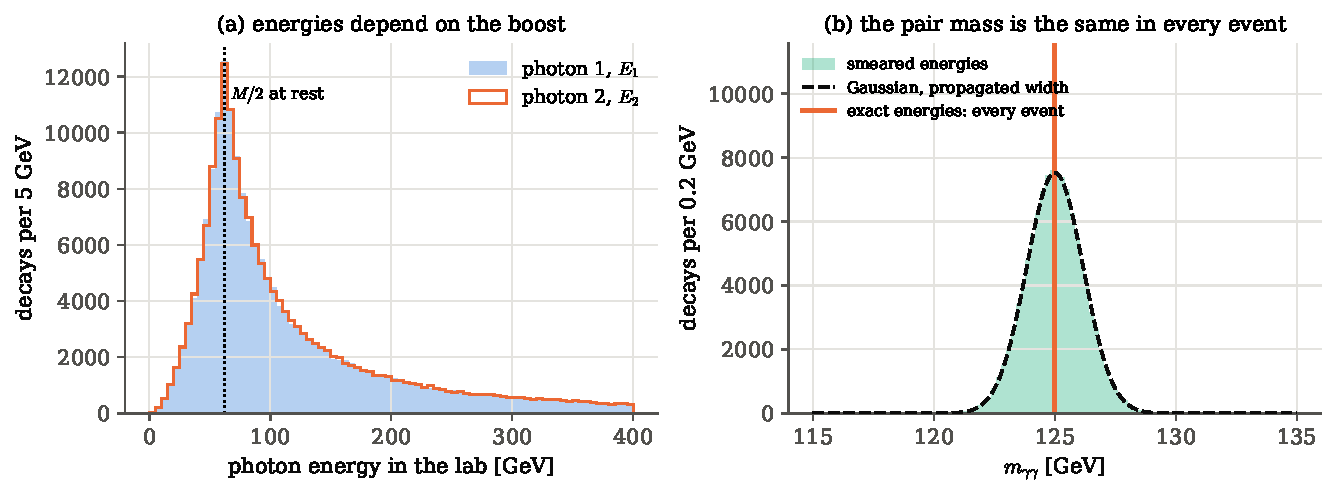
\includegraphics[width=\linewidth]{figures/chT4/mass_from_photons.pdf}
\caption{(a) Photon energies in $\tfouraN{\TfNdecay}$ simulated Higgs decays with random boosts: anywhere from a few tens to several hundred GeV, nowhere near the $62.5$\,GeV of a decay at rest (dotted). (b) The invariant mass of the same pairs. With exact energies every event sits at $125$\,GeV (the vertical line). With energies smeared by the calorimeter resolution the pairs form a peak whose width is predicted by the error propagation \eqref{T4a:eq:mres} (dashed).}
\label{T4a:fig:mass-photons}
\end{figure}

\emph{Natural width and resolution together.} The measured mass is the true mass of the decaying state, distributed as \eqref{T4a:eq:bw}, plus an independent measurement error, roughly Gaussian with width $\sigma_m$. The density of a sum of independent variables is the convolution of their densities, so the observed peak is the Voigt profile of \eqref{2b:eq:voigt-cf}. \emph{Which of the two shapes wins?} It depends on the ratio $\Gamma/\sigma_m$.
\begin{itemize}[itemsep=1pt,leftmargin=1.2em]
  \item \emph{The $Z$ boson.} $\Gamma_Z=2.50$\,GeV and a dielectron mass resolution of about $1.5$\,GeV (CMS quotes $1.56$\,GeV in its barrel \cite[Sec.~3]{ChatrchyanHiggs2012}) are comparable. The full widths at half maximum are $\tfouraR{2}{\TfFwBZ}$\,GeV for the Breit--Wigner alone, $\tfouraR{2}{\TfFwGZ}$\,GeV for the Gaussian alone ($2.355\,\sigma$), and $\tfouraR{2}{\TfFwVZ}$\,GeV for their convolution. Both effects matter, and a fit to the $Z$ peak can separate them because their tails differ.
  \item \emph{The Higgs boson.} $\Gamma_H\approx4$\,MeV against $\sigma_m\approx1.6$\,GeV. The Voigt and the Gaussian of the same $\sigma$ differ by at most $\tfouraR{1}{\TfVHrel}\times100\%$ of the peak height, with half-maximum widths $\tfouraR{3}{\TfFwVH}$ and $\tfouraR{3}{\TfFwGH}$\,GeV. The width of the observed Higgs peak is entirely the detector's \cite[Sec.~4]{ChatrchyanHiggs2012}; the particle's own width cannot be read off it.
\end{itemize}

\begin{keyidea}[Peak position and peak width]
The position of a resonance peak in an invariant-mass histogram measures the particle's mass, because $m_{12}^2=(p_1+p_2)^2=M^2$ in every decay. Its width combines the natural width $\Gamma=\hbar/\tau$ (Breit--Wigner) and the detector resolution $\sigma_m$ (Gaussian core), and is dominated by whichever is larger; for the Higgs boson in two photons it is the resolution, about $1.6$\,GeV, against a natural width of $4$\,MeV.
\end{keyidea}

\emph{Why the Gaussian is not enough: the Crystal Ball.} A Gaussian error assumes many small, symmetric contributions. Some photons, however, lose a sizeable part of their energy before or outside the calorimeter: in the material in front of it, by converting, or by leaking out of the back or the sides of the shower. These losses only go one way, so the measured mass acquires a tail on the low side. ATLAS modelled its signal with a \newterm{Crystal Ball} function, a Gaussian core joined to a power-law tail, with $\sigma_{\rm CB}=1.6$\,GeV and a full width at half maximum of $3.9$\,GeV for the inclusive sample \cite[Sec.~5.4]{AadHiggs2012}. In the standardised variable $t=(m-\bar m)/\sigma$ it is
\begin{equation}
  f(t)\propto
  \begin{cases}
    e^{-t^2/2}, & t>-\alpha,\\
    A\,(B-t)^{-n}, & t\le-\alpha,
  \end{cases}
  \label{T4a:eq:cb}
\end{equation}
where $\alpha>0$ says how many standard deviations below the peak the tail begins, and $n$ how slowly it falls. \emph{What fixes $A$ and $B$?} We require the two pieces to join smoothly at $t=-\alpha$, with the same value and the same slope. The Gaussian piece has value $e^{-\alpha^2/2}$ and slope $-t\,e^{-t^2/2}=\alpha e^{-\alpha^2/2}$ there; the tail piece has value $A(B+\alpha)^{-n}$ and slope $nA(B-t)^{-n-1}=nA(B+\alpha)^{-n-1}$. So
\begin{align}
  A(B+\alpha)^{-n}&\eqby{1}e^{-\alpha^2/2},\qquad
  \frac{n}{B+\alpha}\,e^{-\alpha^2/2}\eqby{2}\alpha\,e^{-\alpha^2/2}
  \nonumber\\
  \Longrightarrow\quad B&\eqby{3}\frac n\alpha-\alpha,\qquad
  A\eqby{4}\Bigl(\frac n\alpha\Bigr)^{n}e^{-\alpha^2/2} .
  \label{T4a:eq:cb-AB}
\end{align}
\begin{explain}
  \item Equal values at $t=-\alpha$.
  \item Equal slopes; the tail slope $nA(B+\alpha)^{-n-1}$ equals $\frac{n}{B+\alpha}A(B+\alpha)^{-n}$, and the first condition replaces $A(B+\alpha)^{-n}$.
  \item Solve the second condition for $B$.
  \item Insert $B+\alpha=n/\alpha$ into the first condition.
\end{explain}
For $\alpha=1.5$ and $n=5$, $B=\tfouraR{3}{\TfBcb}$ and $A=\tfouraR{1}{\TfAcb}$. The tail then carries $\tfouraR{1}{\TfTailFrac}\%$ of the probability, compared with $6.7\%$ for the same region of a Gaussian, while the core, and so the full width at half maximum ($\tfouraR{3}{\TfFwCB}\,\sigma$), is unchanged. Panel (c) of \cref{T4a:fig:lineshapes} shows the difference on a logarithmic scale; it is invisible on a linear one, and yet a few per cent of the signal sits in the tail, where a narrow mass window would lose it.

\begin{figure}[htbp]
\centering
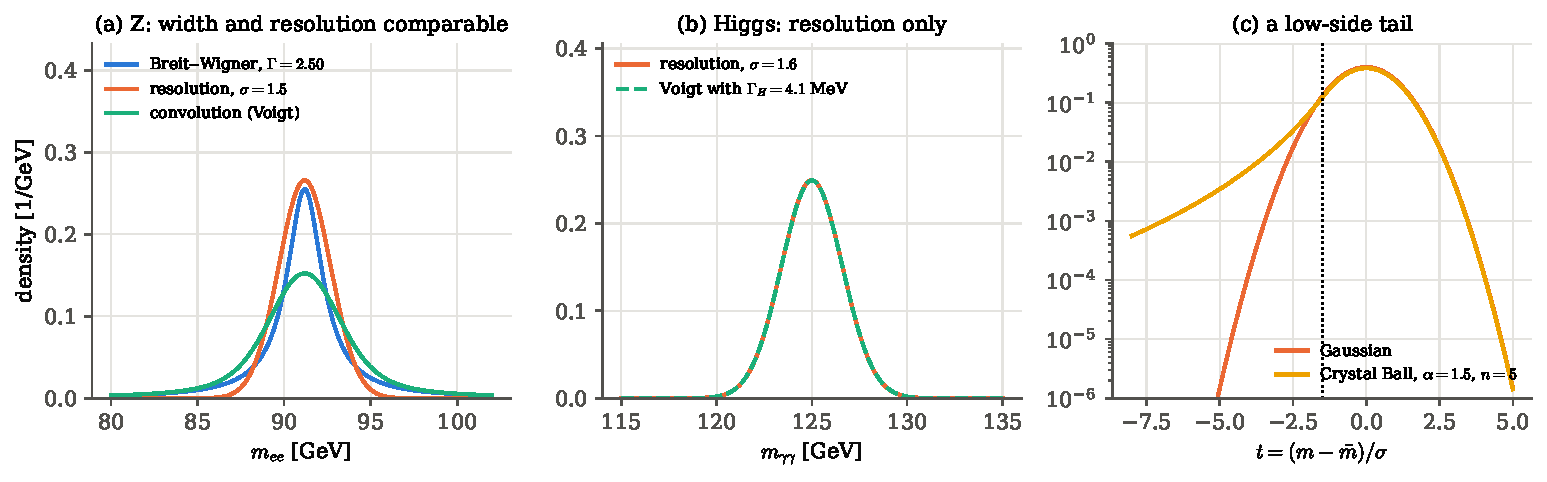
\includegraphics[width=\linewidth]{figures/chT4/line_shapes.pdf}
\caption{Line shapes. (a) For the $Z$ boson, the natural Breit--Wigner width and a $1.5$\,GeV Gaussian resolution are comparable, and the observed peak is their convolution, wider than either. (b) For the Higgs boson the natural width is four hundred times smaller than the resolution; the convolution (dashed) cannot be told apart from the Gaussian. (c) A Crystal Ball function and a Gaussian with the same core, on a logarithmic scale: below $t=-\alpha$ (dotted) the Crystal Ball falls as a power law, modelling photons that lost energy before reaching the calorimeter.}
\label{T4a:fig:lineshapes}
\end{figure}

\paragraph{Where this is used.}
The signal templates of \cref{T4a:sec:templates} and of the capstone (\cref{ch:13}) are peaks of exactly this kind, a Gaussian or Crystal Ball core at the hypothesised mass whose width is set by \eqref{T4a:eq:mres}. The simulated signal of the open data (\cref{T4a:sec:opendata}) has a core of $\tfouraR{2}{\TfdSigMC}$\,GeV and a visible low-side tail. The idea that the detector replaces a true value $y$ by a measured value $x$ with a known probability density, here a Gaussian or a Crystal Ball centred on $y$, is the \emph{resolution function} of the unfolding problem in \cref{6b:sec:unfolding}, where the question is reversed: given the blurred histogram, what was the true one?
\section{Signal and background: where the templates come from}
\label{T4a:sec:templates}

The histogram of the diphoton mass $m_{\gamma\gamma}$ from \cref{T4a:sec:mass} has, say, sixty bins of $1$\,GeV between $100$ and $160$\,GeV. The statistics of \cref{ch:04} needs, for every bin $i$, the number of events $\nu_i$ we \emph{expect} there. Two kinds of events fill the bins: Higgs decays (the signal) and everything else that produces two photon candidates (the background). \Cref{T4a:sec:xsec} gave the total number of each kind, $\nu=\sigma L\varepsilon A$; \cref{T4a:sec:mass} said roughly where the signal lands, in a narrow peak. What is still missing is the full predicted \emph{shape} of each kind, bin by bin, and an honest normalisation of the background. Nobody can write those down from a formula: the shape of a detector's response to millions of different events is not a closed-form function.

\emph{The smallest example: two bins.} Take only two bins. Bin 1 is a $10$\,GeV window around $125$\,GeV, bin 2 is everything else between $100$ and $160$\,GeV. Write the expected counts as
\begin{equation}
  \nu_1=S\,f_1+B\,g_1,\qquad \nu_2=S\,f_2+B\,g_2,
  \label{T4a:eq:two-bin}
\end{equation}
where $S$ and $B$ are the expected total numbers of signal and background events, and $f_j$ and $g_j$ are the fractions of each that fall in bin $j$ (so $f_1+f_2=1$ and $g_1+g_2=1$). There are two kinds of dial. The \emph{normalisations} $S$ and $B$ say how many events of each kind there are; the \emph{shapes} $f_j$ and $g_j$ say how they are shared among the bins. For the open data of \cref{T4a:sec:opendata} the numbers are roughly $S\approx\TfdNexp$, $f_1\approx0.94$, $B\approx\tfouraN{\TfdNsel}$ and $g_1\approx0.17$: about $\tfouraR{0}{\TfdSwin}$ signal events and $\tfouraN{\TfdBwin}$ background events in the window.

\emph{A naive choice: simulate everything.} Suppose we took both $S$ and $B$ from the Standard Model prediction and a simulation of the detector. The background in the window then carries the uncertainty of the background prediction. Most of the background is genuine photon pairs, but about a quarter is jets that the detector mistook for photons (\cref{T4a:sec:bkg-data}), and how often a jet fakes a photon depends on details of jet formation and of the calorimeter response that simulations reproduce far less precisely than the data count events \cite[Sec.~4.2]{Cranmer2015}. Even a $10\%$ error on $B g_1$ is $\num{2600}$ events, seven times the whole expected signal. The peak would drown in the uncertainty of the floor it sits on.

\emph{A better choice, and its price.} The data themselves measure the background: away from $125$\,GeV the histogram contains almost no signal, so the bins on either side of the peak, the \newterm{sidebands}, show how many background events there are and how their number falls with mass. With $\tfouraN{\TfdNsel}$ events the statistical error on the background level is a fraction of a per cent, not ten per cent. The price is an assumption: to carry the background from the sidebands into the window we must assume a smooth shape for it, and a wrong shape can create or hide a few events of fake signal (\cref{T4a:sec:bkg-data}). The signal, on the other hand, has no sidebands; its shape and its expected size can only come from simulation, and its uncertainty is carried by the calibrations of \cref{T4a:sec:nuisance}.

So the division of labour is: signal from simulation, background from the data. Both templates can now be built, and with them the one number the search reports, the signal strength $\mu$. In the language of Cranmer, these are the ``simulation narrative'' and the ``data-driven narrative'' of an analysis \cite[Secs.~4.1--4.2]{Cranmer2015}.

\subsection{Simulated events: from the theory to a detector record}
\label{T4a:sec:simulation}

\emph{The question.} Theory predicts the probability of producing two photons with given momenta. What we need is the probability that the \emph{detector records} a photon pair with a given measured mass. How do we get from one to the other?

The answer is to simulate events one at a time, following each step a real event goes through, and then to histogram the results. A simulated event passes through four programs in turn (\cref{T4a:fig:simchain}) \cite[Sec.~4.1]{Cranmer2015}, \cite[Sec.~3]{AadHiggs2012}.
\begin{enumerate}[itemsep=1pt,leftmargin=1.5em]
  \item \emph{The hard process.} A \newterm{matrix-element generator} draws the momenta of the outgoing particles of the short-distance collision (for the signal, $gg\to H\to\gamma\gamma$) with the probability density predicted by perturbation theory, multiplied by the parton densities of the protons. ATLAS used \textsc{Powheg} for gluon fusion and vector-boson fusion in 2012 \cite[Table~1]{AadHiggs2012}.
  \item \emph{Parton shower and hadronisation.} Quarks and gluons radiate further gluons and then bind into hadrons; programs such as \textsc{Pythia} and \textsc{Herwig} model this with tuned phenomenological parameters. The remnants of the two protons, and the pile-up collisions of \cref{T4a:sec:lumi}, are added here.
  \item \emph{Detector simulation.} \textsc{Geant4} tracks every particle through a model of the detector material and records the energy it deposits in each channel \cite[Sec.~3]{AadHiggs2012}.
  \item \emph{Reconstruction.} The same programs that process real data turn the simulated deposits into photons, electrons, jets, each with its $p_T$, $\eta$ and $\phi$ (\cref{T4a:sec:events}).
\end{enumerate}
Steps 1 and 2 are a model of nature, steps 3 and 4 a model of the experiment. The output has exactly the format of real data, plus the true momenta from step 1, so the same selection can be applied to both.

\begin{figure}[htbp]
\centering
\begin{tikzpicture}[
  st/.style={draw=accent,rounded corners=2pt,fill=ideabg,align=center,font=\small,
             minimum width=2.45cm,minimum height=1.25cm,inner sep=2pt},
  tfnat/.style={st,draw=formblue},
  tfexp/.style={st,draw=bdryred,fill=warnbg},
  tfout/.style={st,draw=tangentgreen,fill=takebg},
  arr/.style={->,thick,accent}]
  \node[tfnat] (hard) at (0,0) {hard process\\ $gg\to H\to\gamma\gamma$\\ {\scriptsize\textsc{Powheg}}};
  \node[tfnat] (show) at (3.15,0) {shower and\\ hadronisation\\ {\scriptsize\textsc{Pythia}}};
  \node[tfexp] (det) at (6.3,0) {detector\\ simulation\\ {\scriptsize\textsc{Geant4}}};
  \node[tfexp] (reco) at (9.45,0) {reconstruction\\ $p_T,\ \eta,\ \phi,\ E$};
  \node[tfout] (sel) at (9.45,-2.4) {same selection\\ as the data};
  \node[tfout] (hist) at (4.725,-2.4) {weighted histogram\\ of $m_{\gamma\gamma}$: $s_i$};
  \node[st] (data) at (9.45,-4.4) {recorded\\ data};
  \draw[arr] (hard) -- (show);
  \draw[arr] (show) -- (det);
  \draw[arr] (det) -- (reco);
  \draw[arr] (reco) -- (sel);
  \draw[arr] (data) -- (sel);
  \draw[arr] (sel) -- (hist);
  \draw[decorate,decoration={brace,amplitude=5pt,raise=3pt},formblue] (-1.25,0.75) -- (4.4,0.75)
     node[midway,above=9pt,font=\scriptsize,formblue] {a model of nature};
  \draw[decorate,decoration={brace,amplitude=5pt,raise=3pt},bdryred] (4.9,0.75) -- (10.7,0.75)
     node[midway,above=9pt,font=\scriptsize,bdryred] {a model of the experiment};
\end{tikzpicture}
\caption{How a signal template is made. Each simulated event passes through the programs that model the collision (blue) and the programs that model the detector (red), and comes out in the same format as a recorded event. The selection used on the data is applied to it unchanged, and the surviving events, each with its weight, are histogrammed to give the expected signal count $s_i$ in every bin.}
\label{T4a:fig:simchain}
\end{figure}

\emph{From simulated events to a shape.} If the detector were perfect, the distribution of an observable $x$ (here $x=m_{\gamma\gamma}$) would be the normalised differential cross section, $f(x)=(1/\sigma_{\rm eff})\,\dd\sigma_{\rm eff}/\dd x$, with $\sigma_{\rm eff}=\sigma\varepsilon A$ the effective cross section of \eqref{T4a:eq:nu} \cite[(17)]{Cranmer2015}. With a real detector there is no formula, but there is a sample: the values $x_1,\dots,x_N$ of the simulated events that pass the selection are draws from the true $f(x)$, and a histogram of them estimates it \cite[(18)]{Cranmer2015}. This is the histogram estimate of a density of \cref{6b:sec:histogram}, with its bin-width trade-off; in a template it is usually harmless, because the bins are chosen narrower than the resolution $\sigma_m$ of \cref{T4a:sec:resolution} and the simulated sample is large.

\paragraph{Example: what the generator list of 2012 says about the backgrounds.}
The ATLAS list of generators \cite[Table~1]{AadHiggs2012} contains one program for the diphoton continuum ($q\bar q/gg\to\gamma\gamma$, \textsc{Sherpa}) and several for processes with a $W$, a $Z$ or top quarks, which matter for the four-lepton and $WW$ channels. It contains no simulation of a photon plus a jet faking a second photon. That background was taken from the data (\cref{T4a:sec:bkg-data}). The list tells us which parts of a search trusted the simulation and which did not.

\subsection{Normalising a weighted simulation}
\label{T4a:sec:weights}

\emph{The question.} A simulated sample has a certain number of events, chosen by whoever generated it; it has nothing to do with the luminosity of the data. \emph{How many real events does one simulated event stand for?}

\emph{The simplest case: unweighted events.} Suppose the generator produced $N_{\rm gen}$ events of a process with cross section $\sigma$, each an independent draw from the produced events. The data contain on average $\sigma L$ produced events of this process. If $N_{\rm sel,i}$ of the simulated events pass the selection and land in bin $i$, the fraction $N_{\rm sel,i}/N_{\rm gen}$ estimates the probability that a produced event does so (a Monte Carlo average of an indicator, as in the acceptance example of \cref{6b:sec:acceptance}). Then $s_i=\sigma L\,N_{\rm sel,i}/N_{\rm gen}$: each simulated event counts for $\sigma L/N_{\rm gen}$ real ones.

\emph{Weighted events.} Modern generators do not produce equal events. A next-to-leading-order generator gives each event a weight $w_e$, sometimes negative, so that the \emph{weighted} sample reproduces the predicted distribution. Later, small corrections that make the simulation agree with calibration data multiply each weight by \newterm{scale factors} (\cref{T4a:sec:opendata}). The fraction of produced events in a region is then the fraction of the total weight in it, and
\begin{align}
  s_i
  &\eqby{1}\sigma L\,\Prob(\text{a produced event is selected and lands in bin }i)
  \nonumber\\
  &\eqby{2}\sigma L\,\frac{\sum_{e\in i}w_e}{\sum_{\text{all }e}w_e}
  \eqby{3}\sum_{e\in i}\Bigl(\frac{\sigma L}{W}\Bigr)w_e,
  \qquad W\equiv\sum_{\text{all }e}w_e .
  \label{T4a:eq:mc-norm}
\end{align}
\begin{explain}
  \item The expected number of produced events is $\sigma L$ (\cref{T4a:sec:xsec}); thinning a Poisson count by a probability gives the expected count in bin $i$.
  \item The probability is estimated by the weighted fraction of simulated events, the self-normalised estimator of \cref{6b:sec:self-norm}. The denominator runs over \emph{all} generated events, before any selection; otherwise the efficiency would be lost.
  \item Bring the constant inside the sum: every selected event contributes $\sigma L\,w_e/W$ expected real events.
\end{explain}
With all $w_e=1$, $W=N_{\rm gen}$ and \eqref{T4a:eq:mc-norm} is the unweighted rule. The capstone uses exactly this formula (\cref{13d:sec:data}).

\emph{How precise is a simulated template?} The simulated sample is finite, so $s_i$ has a statistical error of its own. Think of the simulated events landing in bin $i$ as a Poisson number $K$ of events with mean $\lambda$, each carrying an independent weight $w$. The sum $S_i=\sum_{k=1}^{K}w_k$ then has
\begin{align}
  \Var(S_i)
  &\eqby{1}\E\bigl[\Var(S_i\given K)\bigr]+\Var\bigl[\E(S_i\given K)\bigr]
  \eqby{2}\E[K]\Var(w)+\Var(K)\bigl(\E w\bigr)^2
  \nonumber\\
  &\eqby{3}\lambda\bigl[\Var(w)+(\E w)^2\bigr]
  \eqby{4}\lambda\,\E[w^2]
  \;\approx\;\sum_{e\in i}w_e^2 .
  \label{T4a:eq:mc-stat}
\end{align}
\begin{explain}
  \item The law of total variance \eqref{1b:eq:total-var}, conditioning on the number of events $K$.
  \item Given $K$, the sum of $K$ independent weights has variance $K\Var(w)$ and mean $K\E w$.
  \item $K$ is Poisson, so $\E K=\Var K=\lambda$.
  \item $\Var(w)+(\E w)^2=\E[w^2]$; the expected sum of squared weights $\lambda\E[w^2]$ is estimated by the observed one.
\end{explain}
So the Monte Carlo error of $s_i$ is $(\sigma L/W)\sqrt{\sum_{e\in i}w_e^2}$. For unit weights it is $(\sigma L/N_{\rm gen})\sqrt{N_{\rm sel,i}}$, the familiar $1/\sqrt N$ of a count. Unequal weights make it larger, as if the sample contained only $N_{\rm eff}=\bigl(\sum w_e\bigr)^2/\sum w_e^2$ equal events.

\paragraph{Example: the expected Higgs signal in the open data.}
The gluon-fusion file of the open data (\cref{T4a:sec:opendata}) stores $\sigma B=\TfdXsecTree$\,pb and the sum of the weights of all generated events, $W=\tfouraN{\TfdSumwTree}$. It contains $\tfouraN{\TfdNmc}$ events, those that survived a two-photon preselection. With $L=10\,\mathrm{fb^{-1}}=\num{10000}\,\mathrm{pb^{-1}}$ each unit of weight stands for $\sigma BL/W=0.102\times\num{10000}/\num{55922616}=1.82\times10^{-5}$ real events. The selection of \cref{T4a:sec:eff} keeps a weighted fraction $\varepsilon A=\TfdEffA$, so
\begin{equation*}
  \nu_S=\sigma B\,L\,\varepsilon A=\TfdNprod\times\TfdEffA=\TfdNexp
\end{equation*}
selected signal events between $100$ and $160$\,GeV, with a Monte Carlo error from \eqref{T4a:eq:mc-stat} of $\tfouraR{2}{\TfdNmcstat}$ events. That error is a tenth of a per cent: with a million simulated events, the template's own statistical error is negligible next to the Poisson fluctuation of the data in the same region (about $160$ events, \cref{T4a:sec:bkg-data}). For small simulated samples it is not negligible, and HistFactory gives each bin a nuisance parameter for it, constrained by a Poisson term whose effective count is $(s_i/\delta s_i)^2$ \cite[(9)]{HistFactory2012}.\footnote{The text of \cite[Sec.~2.2.1]{HistFactory2012} writes the effective count as $(\delta_b/\nu_b^{\rm MC})^2$, the inverse; the next sentence there, $\tau_b=(\nu_b^{\rm MC}/\delta_b)^2$, has it the right way round. For unit weights, $(s_i/\delta s_i)^2=N_{\rm sel,i}$, as it should be.}

\paragraph{Example: several processes in one template.}
The signal has four production modes (gluon fusion, vector-boson fusion, and production with a $W$ or a $Z$; \cref{T4a:sec:higgs}), each simulated in its own file with its own $\sigma$ and $W$. Processes that do not interfere quantum mechanically add incoherently, so their expected counts add bin by bin, $s_i=\sum_{\rm samples}s_i^{(k)}$, and the normalised shape is the mixture $f(x)=\sum_k\nu_kf_k(x)/\sum_k\nu_k$ \cite[(20)--(21)]{Cranmer2015}, \srcref{Cowan}{\S6.9}. Processes that \emph{do} interfere must be simulated together as one sample. The 2012 analysis is an example: gluon fusion to a Higgs boson and gluon fusion directly to two photons lead to the same final state, their amplitudes interfere destructively, and ATLAS lowered the gluon-fusion rate by $2$--$5\%$ to account for it \cite[Sec.~5.4]{AadHiggs2012}.

\subsection{The background from the data: sidebands}
\label{T4a:sec:bkg-data}

\emph{What is in the background?} Three kinds of event give two photon candidates. Real photon pairs from quark--antiquark annihilation or gluon fusion through a quark loop (the \emph{irreducible} background, $\gamma\gamma$). A photon and a jet in which one hadron, typically a neutral pion decaying to two nearly collinear photons, looks like a single photon ($\gamma j$). Two such jets ($jj$). The last two are \emph{reducible}: better identification and isolation reduce them. ATLAS measured the composition of its selected 2012 sample with data-driven techniques: $74\%$ $\gamma\gamma$, $22\%$ $\gamma j$, $3\%$ $jj$ and $1\%$ Drell--Yan electron pairs mistaken for photons \cite[Sec.~5.2]{AadHiggs2012}. That decomposition was used only to study the background shape; the search itself fitted the background directly to the data.

\emph{The method.} In every event category ATLAS fitted the $m_{\gamma\gamma}$ spectrum between $100$ and $160$\,GeV with a smooth function whose parameters were free: a fourth-order Bernstein polynomial, the exponential of a second-order polynomial, or a single exponential, depending on the category \cite[Sec.~5.5]{AadHiggs2012}. The function plays the role of the background template $b_i$, with its normalisation and shape parameters measured by the data themselves. Cranmer calls this the ``effective model narrative'': no physical model of the background, only a flexible enough curve \cite[Secs.~4.2--4.3]{Cranmer2015}.

\emph{What could go wrong: the spurious signal.} A smooth function that is not flexible enough can bend away from the true background shape near $125$\,GeV and leave a deficit or excess there that the fit then attributes to signal. ATLAS measured this directly. They fitted signal plus background models to very large simulated background samples, which contain no signal at all, and recorded the largest fitted ``signal'' over the mass range \cite[Sec.~5.5]{AadHiggs2012}. A function was accepted only if this \newterm{spurious signal} was below $20\%$ of the statistical error of the fitted signal; the remaining spurious signal, $0.2$--$4.6$ events at $7$\,TeV and $0.3$--$6.8$ events at $8$\,TeV depending on the category, was kept as a systematic uncertainty. The capstone repeats this test on the open data (\cref{13d:sec:spurious}).

\paragraph{Example: an exponential through the sidebands of the open data.}
As an illustration, the script \pyname{02_open_data.py} of \cref{T4a:sec:opendata} histograms the $\tfouraN{\TfdNsel}$ selected diphoton masses of the 2016 open data in $1$\,GeV bins and, without a proper fit or uncertainties, draws a straight line through the logarithm of the counts in the bins outside $120$--$130$\,GeV. The slope is $\tfouraR{4}{\TfdSlope}$ per GeV: the background falls by $2.3\%$ for every GeV of mass. Extrapolated into the window, the exponential predicts $b=\tfouraN{\TfdBwin}$ background events between $120$ and $130$\,GeV, where $\tfouraN{\TfdNwin}$ events were recorded. The simulated Standard Model signal from \cref{T4a:sec:weights}, histogrammed with \eqref{T4a:eq:mc-norm}, puts $s=\tfouraR{1}{\TfdSwin}$ expected events in the same window. Panel (a) of \cref{T4a:fig:opendata-mgg} shows the three side by side.

The numbers give the problem its size. The signal is $s/b=\tfouraR{2}{\TfdSoverB}\%$ of the background in the window, far too small to see by eye; the typical Poisson fluctuation of the background count is $\sqrt b=162$ events; and the ratio $s/\sqrt b=\tfouraR{2}{\TfdZsimple}$ is the rough number of such fluctuations the expected signal amounts to. Whether that is enough, and how much better the full histogram does than one window, is decided by the statistic $q_0$ and its Asimov approximation in \cref{4b:sec:limits,4b:sec:asimov}. The excess of recorded over predicted events, $\tfouraN{\TfdNwin}-\tfouraN{\TfdBwin}=203$, is about one such fluctuation.

\begin{figure}[htbp]
\centering
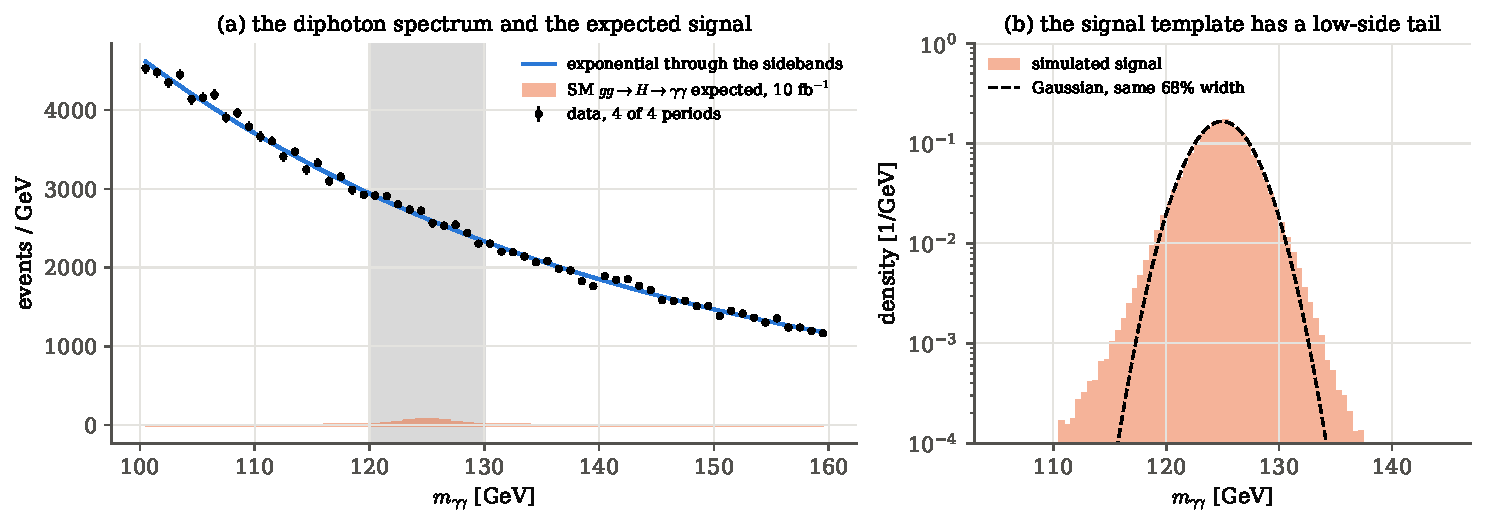
\includegraphics[width=\linewidth]{figures/chT4/opendata_mgg.pdf}
\caption{(a) The diphoton mass spectrum of the 2016 open data after the selection of \cref{T4a:sec:eff}, with an exponential drawn through the sidebands outside the grey window, and the expected Standard Model gluon-fusion signal (filled) at the bottom of the plot: a few dozen events per GeV under a background of thousands. (b) The simulated signal shape on a logarithmic scale against a Gaussian of the same central $68\%$ width. The core is Gaussian; the low-mass side has the tail of photons that lost energy, the shape the Crystal Ball of \eqref{T4a:eq:cb} was built for.}
\label{T4a:fig:opendata-mgg}
\end{figure}

\paragraph{Example: the signal template's width and tail.}
Panel (b) of \cref{T4a:fig:opendata-mgg} is the signal template of the open data. Its median is $\tfouraR{1}{\TfdMedMC}$\,GeV and half of its central $68\%$ range is $\tfouraR{2}{\TfdSigMC}$\,GeV. Of the weighted signal, $\tfouraR{1}{\TfdFracTwo}\%$ lies within two such widths of the median (a Gaussian would have $95.4\%$), $\tfouraR{2}{\TfdLowTail}\%$ lies more than three widths below and $\tfouraR{2}{\TfdHighTail}\%$ more than three widths above (a Gaussian would have $0.13\%$ on each side). This half-width is not the same quantity as the Crystal Ball core width $\sigma_{\rm CB}=1.6$\,GeV of the 2012 analysis: the central $68\%$ range includes part of the tails, which a core width ignores. The asymmetry of the tails is the energy loss described in \cref{T4a:sec:resolution}; \cref{13d:sec:signal-shape} fits the shape properly.

\subsection{The signal strength}
\label{T4a:sec:mu}

\emph{The question.} The search must be able to say ``there is no signal'', ``there is the predicted signal'', and anything in between or beyond. \emph{Which single number expresses that?}

For a fixed hypothesised mass $m_H$, the Standard Model fixes the cross section of every production mode, every branching fraction, and so the size and shape of the signal template. The searches of 2012 therefore did not fit the Higgs couplings themselves. They introduced one factor that scales the predicted signal \cite[Sec.~4.1.2.1]{Cranmer2015}, \cite[Sec.~7]{AadHiggs2012}:
\begin{equation}
  \mu=\frac{\sigma\,B}{(\sigma\,B)_{\rm SM}},
  \qquad
  \nu_i(\mu)=\mu\,s_i+b_i,
  \qquad
  s_i=(\sigma B)_{\rm SM}\,L\,\varepsilon A\,f_i .
  \label{T4a:eq:mu}
\end{equation}
Here $s_i$ is the Standard Model signal template in bin $i$ (the expected count \eqref{T4a:eq:mc-norm}, with the fraction $f_i$ of the selected signal falling in that bin), $b_i$ the background template, and $\mu$ the \newterm{signal strength}. The value $\mu=0$ is the background-only hypothesis, the null hypothesis of the discovery test; $\mu=1$ is the Standard Model Higgs boson; any other value is a signal of the predicted shape but a different size. The second relation is the template model \eqref{4b:eq:nu-template} of \cref{4b:sec:templates}, where its likelihood is written down.

\begin{workdef}[signal strength]
The \newterm{signal strength} $\mu$ is the ratio of the true signal rate to the Standard Model prediction for the same mass hypothesis, $\mu=\sigma B/(\sigma B)_{\rm SM}$ \unpack{cross section times branching fraction into the final state that is searched}. \emph{Operationally:} multiply the simulated signal template by $\mu$, add the background template, and compare with the data bin by bin, $\nu_i=\mu s_i+b_i$.
\end{workdef}

\emph{What $\mu$ can and cannot tell apart.} A diphoton search counts events of production times decay, so it measures only the product $\sigma B$. A Higgs boson produced twice as often and decaying to photons half as often gives the same $\mu=1$. Nor can it tell $\mu$ from anything else that multiplies the signal: a luminosity or a photon efficiency $10\%$ higher than assumed gives exactly the same histogram as a $\mu$ $10\%$ higher. Only an independent calibration separates the two, which is why every such factor enters the search as a nuisance parameter with its own calibration measurement (\cref{T4a:sec:nuisance}). Finally, one $\mu$ for all production modes is a convenience; a theory beyond the Standard Model would change the modes differently, and once a signal was seen ATLAS also fitted separate strengths $\mu_i=\sigma_i/\sigma_{i,\rm SM}$ for groups of modes \cite[Sec.~9.3]{AadHiggs2012}.

\paragraph{Example: what $\mu=1.4$ would mean in the open data.}
ATLAS measured $\hat\mu=1.4\pm0.3$ in 2012 (\cref{T4a:sec:higgs}). If the true signal strength were $1.4$, the $120$--$130$\,GeV window of the open data would hold $1.4\times\tfouraR{1}{\TfdSwin}=520$ signal events on top of the background instead of $\tfouraR{0}{\TfdSwin}$, a difference of $150$ events: less than one Poisson fluctuation of the background count ($162$). A single window of the open data cannot distinguish $\mu=1$ from $\mu=1.4$; the full histogram and the precise statistics of \cref{4b:sec:templates} are needed even to see the signal.

\begin{keyidea}[Signal from simulation, background from the data]
The expected count in bin $i$ is $\nu_i=\mu s_i+b_i$. The signal template $s_i$ is a weighted histogram of simulated events, normalised by $\sigma L w_e/W$ per event; the background template $b_i$ is a smooth function whose parameters are measured by the sidebands of the data. The signal strength $\mu=\sigma B/(\sigma B)_{\rm SM}$ scales the predicted signal: $\mu=0$ is no signal, $\mu=1$ the Standard Model.
\end{keyidea}

\paragraph{Where this is used.}
The template model $\nu_i=\mu s_i+b_i$ and its Poisson likelihood are \cref{4b:sec:templates,4b:sec:binned-like}; the scan of a peak template over the mass axis is \cref{4b:sec:scan}. The capstone builds the signal template from the four simulated production modes with \eqref{T4a:eq:mc-norm} and fits the background shape to the sidebands (\cref{13d:sec:shapes,13d:sec:signal-shape}). The response of a detector to a true value, which the simulation chain of \cref{T4a:fig:simchain} encodes, is the response matrix of the unfolding problem in \cref{6b:sec:unfolding} \srcref{Cowan}{\S11.1}.
\section{Systematic uncertainties: nuisance parameters and their calibrations}
\label{T4a:sec:nuisance}

Every ingredient of the expected count $\nu_i=\mu s_i+b_i$ of \cref{T4a:sec:templates} was measured or computed by someone, and none exactly. The luminosity $L$ came from a calibration of the beams, the photon efficiency from a study of electrons, the energy scale that places the peak from the $Z$ boson, the cross section from a perturbative calculation truncated at some order. \emph{How does each of these imperfections enter the prediction, and what keeps it under control?}

\emph{The smallest example: one bin, one calibration.} Take a single counting window with expected count $\nu=\mu\,\kappa\,s+b$. Here $s$ is the nominal Standard Model signal in the window, $b$ the background, and $\kappa$ the ratio of the true value of luminosity times efficiency to the value assumed when $s$ was computed; $\kappa=1$ if the calibrations were perfect. The two dials $\mu$ and $\kappa$ appear only as their product. Any data in this window are explained equally well by $(\mu,\kappa)=(1.4,1)$ and by $(1,1.4)$.

\emph{The naive choice.} Fix $\kappa=1$ and ignore it. If the true luminosity times efficiency is in fact $11\%$ lower, the fitted $\mu$ comes out $11\%$ low, and no amount of data reveals it: more events only make the wrong answer more precise.

\emph{The better choice, and its price.} Measure $\kappa$ separately, in a calibration that does not involve the Higgs signal at all, and carry its result and its error into the search. Then $\mu\kappa$ is measured by the window and $\kappa$ by the calibration, and $\mu$ follows. The price is a floor on the precision. With infinite data in the window the product $\mu\kappa$ is known exactly, and the relative error on $\mu$ is still the relative error of the calibration. For the diphoton search of 2012, the photon efficiency alone was known to $11\%$ at $8$\,TeV \cite[Sec.~5.6]{AadHiggs2012}, so $\mu$ could not have been measured better than about $11\%$ however many collisions were recorded.

The lesson: a parameter the data cannot separate from the signal must be pinned down by its own measurement, and that measurement's precision becomes part of the result. Each such parameter is a \newterm{nuisance parameter} \unpack{a parameter the prediction depends on and that we must fit, but do not want to report}, and the measurement that pins it down is an \newterm{auxiliary} or \newterm{calibration measurement} \cite[Sec.~2.2]{Cranmer2015}, \cite[\S40.2.2.2]{PDG2024}. A diphoton search has about a dozen such parameters, each with a size, an effect on the templates and a calibration behind it.

\subsection{Sources and their effects}
\label{T4a:sec:sources}

Cranmer makes one distinction the bookkeeping depends on: the \emph{source} of an uncertainty (for example, the calorimeter's energy calibration) is not the same thing as its \emph{effect} on a particular template (the signal peak moves; the background shape hardly changes) \cite[Sec.~4.1.4]{Cranmer2015}. One source gets one nuisance parameter, even if it affects many templates, channels and data sets. ATLAS treated the luminosity as fully correlated across the diphoton, four-lepton and $WW$ channels, and the photon and electron energy scales as five shared parameters \cite[Sec.~8]{AadHiggs2012}. The effects come in three kinds, which HistFactory calls by the names in brackets \cite[Table~1]{HistFactory2012}:
\begin{itemize}[itemsep=1pt,leftmargin=1.2em]
  \item \emph{Normalisation} (\texttt{OverallSys}): the whole template is multiplied by a factor near one. Luminosity, efficiencies and cross sections act this way.
  \item \emph{Shape} (\texttt{HistoSys}): the fractions $f_i$ themselves change. The energy scale moves the peak; the resolution widens or narrows it.
  \item \emph{Bin by bin} (\texttt{StatError}, \texttt{ShapeSys}): each bin gets its own factor, for example for the finite simulated sample of \eqref{T4a:eq:mc-stat}.
\end{itemize}
\Cref{T4a:fig:sources} draws the sources of the 2012 diphoton search with the effect each one has.

\begin{figure}[htbp]
\centering
\begin{tikzpicture}[
  src/.style={draw=bdryred,fill=warnbg,rounded corners=2pt,font=\small,align=left,
              minimum width=4.6cm,minimum height=0.62cm,inner sep=2pt,anchor=west},
  eff/.style={draw=formblue,fill=ideabg,rounded corners=2pt,font=\small,align=center,
              minimum width=3.0cm,minimum height=0.9cm,inner sep=2pt},
  ln/.style={thick,softgray}]
  \node[src] (lum) at (0,0)    {luminosity \hfill $1.8\%$, $3.6\%$};
  \node[src] (eff) at (0,-0.85) {photon efficiency \hfill $8\%$, $11\%$};
  \node[src] (th)  at (0,-1.7) {cross section, $B$ \hfill $\approx12\%$};
  \node[src] (pu)  at (0,-2.55) {pile-up modelling \hfill $4\%$};
  \node[src] (res) at (0,-3.4) {energy resolution \hfill $14\%$};
  \node[src] (esc) at (0,-4.25) {energy scale \hfill $\approx0.3\%$};
  \node[src] (bkg) at (0,-5.1) {background function \hfill $\lesssim7$ ev.};
  \node[eff] (norm) at (8.6,-1.275) {signal yield\\ (normalisation)};
  \node[eff] (wid)  at (8.6,-3.0) {peak width\\ (shape)};
  \node[eff] (pos)  at (8.6,-4.25) {peak position\\ (shape)};
  \node[eff] (sp)   at (8.6,-5.3) {fake signal\\ (spurious)};
  \foreach \s in {lum,eff,th,pu} \draw[ln] (\s.east) -- (norm.west);
  \draw[ln] (esc.east) -- (pos.west);
  \draw[ln] (res.east) -- (wid.west);
  \draw[ln] (pu.east) -- (wid.west);
  \draw[ln] (bkg.east) -- (sp.west);
\end{tikzpicture}
\caption{The main sources of systematic uncertainty in the 2012 diphoton search (left, with their sizes; two numbers are for the $7$ and $8$\,TeV data) and the effect each has on the templates (right). Most sources only rescale the expected signal. The energy scale moves the peak, the resolution changes its width, and pile-up does both. The background function's uncertainty is a number of events of spurious signal per category.}
\label{T4a:fig:sources}
\end{figure}

\paragraph{Example: why the photon efficiency counts twice.}
Every selected event has two photons, and each passes the identification with probability $\varepsilon_\gamma$, so the yield is proportional to $\varepsilon_{\gamma1}\varepsilon_{\gamma2}$. A calibration error that moves both efficiencies in the same direction by $\delta\varepsilon_\gamma/\varepsilon_\gamma$ changes the yield by
\begin{align}
  \frac{\delta\nu}{\nu}
  \eqby{1}\frac{\delta\varepsilon_{\gamma1}}{\varepsilon_{\gamma1}}+\frac{\delta\varepsilon_{\gamma2}}{\varepsilon_{\gamma2}}
  \eqby{2}2\,\frac{\delta\varepsilon_\gamma}{\varepsilon_\gamma} .
  \label{T4a:eq:eff-twice}
\end{align}
\begin{explain}
  \item The logarithm of a product is the sum of the logarithms; differentiate.
  \item The same calibration applies to both photons, so the two errors are equal and add linearly, not in quadrature.
\end{explain}
A per-photon uncertainty of $5.5\%$ thus becomes the $11\%$ on the yield quoted for the $8$\,TeV data.

\paragraph{Example: adding up the yield uncertainties.}
For the $8$\,TeV diphoton signal the experimental normalisation uncertainties are the photon efficiency ($11\%$), pile-up ($4\%$), luminosity ($3.6\%$), trigger ($1\%$) and isolation ($0.5\%$) \cite[Sec.~5.6]{AadHiggs2012}; the theory uncertainties on the gluon-fusion prediction are the QCD scale ($+7/{-8}\%$, about $7.5\%$), the parton densities ($8\%$) and the branching fraction ($5\%$) \cite[Sec.~8]{AadHiggs2012}. The sources are independent, so their variances add (\cref{3a:sec:propagation}):
\begin{align}
  \Bigl(\frac{\delta\nu}{\nu}\Bigr)_{\rm exp}
  &\eqby{1}\sqrt{11^2+4^2+3.6^2+1^2+0.5^2}\,\%=12.3\%,
  \nonumber\\
  \Bigl(\frac{\delta\nu}{\nu}\Bigr)_{\rm th}
  &\eqby{1}\sqrt{7.5^2+8^2+5^2}\,\%=12.1\%,
  \qquad
  \Bigl(\frac{\delta\nu}{\nu}\Bigr)_{\rm tot}\eqby{2}\sqrt{12.3^2+12.1^2}\,\%=17\% .
  \label{T4a:eq:quadrature}
\end{align}
\begin{explain}
  \item Independent relative errors on factors of a product add in quadrature.
  \item The experimental and theoretical groups are independent of each other as well.
\end{explain}
The one large experimental term dominates its group: removing the luminosity entirely would lower $12.3\%$ only to $11.8\%$. This is typical of quadrature sums and tells an analysis where improvement pays.

\paragraph{Example: the peak moves with the energy scale.}
Suppose every measured photon energy is too large by the same fraction $\delta$: $E_j\to(1+\delta)E_j$. The angle between the photons is unchanged, so by \eqref{T4a:eq:mgg-angle}
\begin{align}
  m_{\gamma\gamma}'^{\,2}
  \eqby{1}2\,(1+\delta)E_1\,(1+\delta)E_2\,(1-\cos\theta_{12})
  \eqby{2}(1+\delta)^2\,m_{\gamma\gamma}^2,
  \qquad\text{so}\qquad
  \frac{\delta m}{m}=\delta .
  \label{T4a:eq:scale-shift}
\end{align}
\begin{explain}
  \item Insert the scaled energies into $m^2=2E_1E_2(1-\cos\theta_{12})$.
  \item Factor out $(1+\delta)^2$; the square root gives $m'=(1+\delta)m$.
\end{explain}
A common scale error moves the whole peak by the same fraction and leaves its relative width unchanged. ATLAS quoted a systematic error of $0.4$\,GeV on the mass $126.0$\,GeV, dominated by the photon and electron energy scales \cite[Sec.~9.3]{AadHiggs2012}: a scale known to about $0.3\%$. That is $0.3\%\times125=\tfouraR{3}{\TfShiftGeV}$\,GeV of peak shift, a quarter of the peak's width.

\emph{What the three kinds of effect look like.} The script \pyname{01_mass_lineshape.py} takes a Crystal Ball signal template of core width $1.6$\,GeV, the shape of \eqref{T4a:eq:cb} with the 2012 width, and applies a $\pm0.3\%$ energy-scale shift, a $\pm14\%$ resolution change (the total ATLAS uncertainty on the mass resolution, itself the quadrature sum $\sqrt{12^2+6^2+4^2}=14$ of calorimeter resolution, detector material and pile-up \cite[Sec.~5.6]{AadHiggs2012}) and a $\pm11\%$ yield change (\cref{T4a:fig:systvar}). The fraction of the signal inside a $\pm2$\,GeV window around $125$\,GeV is $\tfouraR{1}{\TfWinNom}\%$ nominally, $\tfouraR{1}{\TfWinResUp}\%$ and $\tfouraR{1}{\TfWinResDn}\%$ for the wider and narrower peak, and $\tfouraR{1}{\TfWinShift}\%$ after the scale shift. A shape uncertainty is therefore also a normalisation uncertainty for any analysis that counts in a fixed window, and the two must not be counted twice.

\begin{figure}[htbp]
\centering
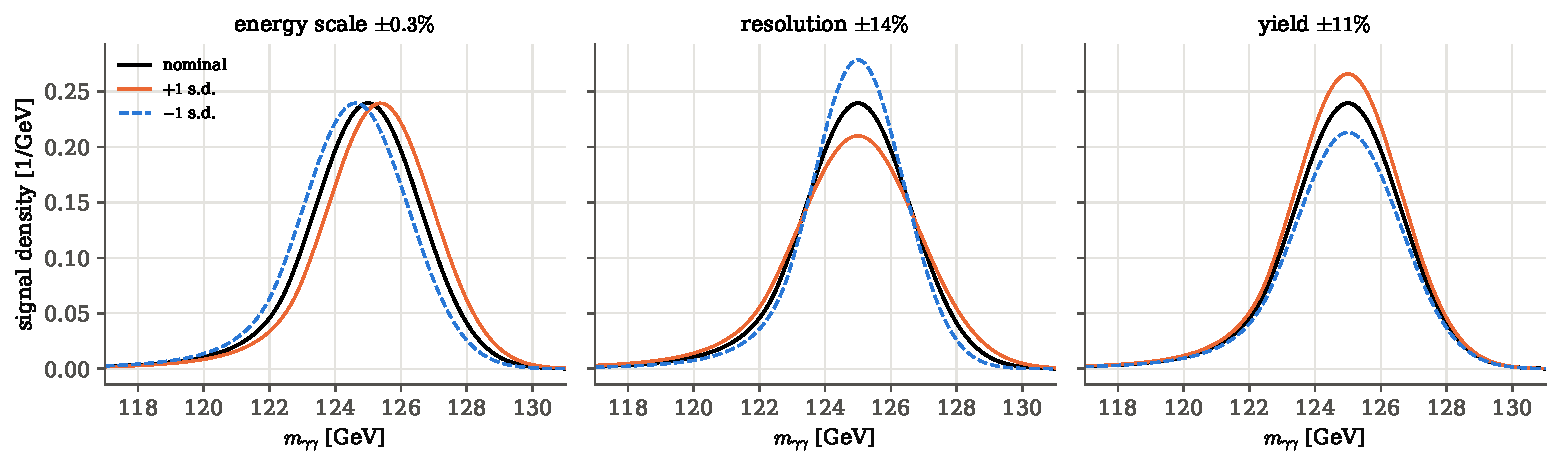
\includegraphics[width=\linewidth]{figures/chT4/syst_variations.pdf}
\caption{The three effects of a systematic uncertainty on a signal template, with ``up'' and ``down'' variations by one standard deviation. Left: an energy-scale shift of $0.3\%$ slides the peak sideways by $0.4$\,GeV. Middle: a $14\%$ change of the resolution makes the peak wider and lower, or narrower and taller, with the same area. Right: an $11\%$ change of the yield rescales the peak without changing its shape.}
\label{T4a:fig:systvar}
\end{figure}

\subsection{From up and down variations to a continuous parameter}
\label{T4a:sec:interp}

\emph{The question.} A calibration study delivers, for each source, the template at its nominal value and at ``plus one'' and ``minus one'' standard deviation. The likelihood of \cref{ch:04} needs the template at \emph{every} value of the nuisance parameter. \emph{How is the gap filled?}

The convention is to define a parameter $\alpha$ for each source (not the tail parameter of the Crystal Ball \eqref{T4a:eq:cb}) with $\alpha=0$ the nominal value and $\alpha=\pm1$ the one-standard-deviation variations, and to interpolate. The simplest rule, used for a normalisation factor $r(\alpha)$ with variations $r^\pm$ (HistFactory calls it $\eta$, which here would be confused with the pseudorapidity), is piecewise linear \cite[(23)--(25)]{Cranmer2015}:
\begin{equation}
  r(\alpha)=
  \begin{cases}
    1+\alpha\,(r^+-1), & \alpha\ge0,\\
    1+\alpha\,(1-r^-), & \alpha<0,
  \end{cases}
  \label{T4a:eq:interp}
\end{equation}
and the same rule, bin by bin, interpolates the up and down templates of a shape uncertainty. For the $8$\,TeV luminosity, $r^\pm=1\pm0.036$; half a standard deviation up, $\alpha=0.5$, scales the signal by $1.018$. HistFactory assembles all of this into one expression for the expected count of sample $s$ in bin $b$ \cite[(6)]{HistFactory2012},
\begin{equation}
  \nu_{sb}=\lambda\;\gamma_b\;\phi_s\;r_s(\bm\alpha)\;\sigma_{sb}(\bm\alpha),
  \label{T4a:eq:histfactory}
\end{equation}
which reads, in our notation: the luminosity $\lambda=L$; a per-bin factor $\gamma_b$ for the Monte Carlo statistics; free factors $\phi_s$, of which the signal strength $\mu$ is one; the interpolated normalisation \eqref{T4a:eq:interp} (HistFactory's $\eta_s$); and the interpolated template $\sigma_{sb}$, our $s_i$ or $b_i$. Every factor except $\phi_s$ comes with a constraint from its calibration.

\begin{pitfall}[An up/down pair is not a measurement of the shape]
Interpolating between three templates assumes the template changes smoothly and, in each bin separately, roughly linearly with $\alpha$. A peak that \emph{moves} violates this: halfway between a template shifted left and one shifted right, bin-by-bin interpolation gives a broadened or even two-humped peak, not a peak shifted halfway. Cranmer points to ``horizontal'' interpolation for such cases \cite[Sec.~4.1.5]{Cranmer2015}; the diphoton searches sidestep it because their signal model is an analytic function of the mass, whose mean can simply be shifted, $f(m\given\bar m(1+\delta),\sigma_m)$.
\end{pitfall}

\subsection{Calibrations: how a nuisance parameter is measured}
\label{T4a:sec:calib}

A nuisance parameter is only as good as the measurement that constrains it. Two calibrations matter most for a diphoton search: the luminosity, which sets every normalisation, and the photon energy scale, which places the peak.

\paragraph{The luminosity: a van der Meer scan.}
\Cref{T4a:sec:lumi} derived the luminosity from the overlap of two bunches, $L_{\rm inst}\propto N_1N_2\int\rho_1\rho_2\,\dd x\,\dd y$. The bunch populations $N_1$, $N_2$ are measured by current monitors on the beams. The overlap integral is the hard part: the transverse sizes of the beams at the collision point, a few tens of micrometres, cannot be measured directly with the needed precision. Van der Meer's idea is to measure the overlap by moving the beams. \emph{What happens to the rate of collisions when one beam is displaced sideways by $\Delta$?}

Let the $x$ profiles of the two bunches be Gaussians of widths $s_1$ and $s_2$. The $x$ part of the overlap at separation $\Delta$ is $\int g(x;s_1)\,g(x-\Delta;s_2)\,\dd x$. This is the convolution integral \eqref{1b:eq:convolution}: it is the probability density, at the value $\Delta$, of the difference $X_1-X_2$ of two independent Gaussian positions. A difference of independent Gaussians is Gaussian with the variances added, so
\begin{equation}
  \int g(x;s_1)\,g(x-\Delta;s_2)\,\dd x
  =\frac{1}{\sqrt{2\pi}\,\Sigma_x}\,e^{-\Delta^2/2\Sigma_x^2},
  \qquad
  \Sigma_x=\sqrt{s_1^2+s_2^2} .
  \label{T4a:eq:vdm}
\end{equation}
For equal beams, $\Sigma_x=\sqrt2\,\sigma_x$ and this is \eqref{T4a:eq:overlap-x}. The rate $R$ of any process seen by a luminosity detector is proportional to the overlap, so scanning $\Delta$ and recording $R(\Delta)$ traces a Gaussian whose width is $\Sigma_x$. A second scan in $y$ gives $\Sigma_y$. With them the head-on luminosity of one pair of bunches is known in absolute terms, $L_0=fN_1N_2/(2\pi\Sigma_x\Sigma_y)$, and the peak rate of the scan defines the detector's \newterm{visible cross section} $\sigma_{\rm vis}=R_0/L_0$. From then on, in ordinary running, every measured rate converts to a luminosity as $L_{\rm inst}=R/\sigma_{\rm vis}$.

\emph{The toy scan.} The script \pyname{03_luminosity.py} simulates such a scan for one pair of LHC design bunches ($\sigma_x=16.7\,\mu$m, so $\Sigma_x=\tfouraR{2}{\TflSigmaTrue}\,\mu$m) and a luminosity detector with $\sigma_{\rm vis}=\TflSigVisTrue$\,mb. It counts Poisson events for $\TflTpoint$\,s at each of $\TflNpoints$ separations between $\pm5\Sigma_x$ and fits a Gaussian to the rates (\cref{T4a:fig:vdm}). The fit returns $\Sigma_x=\tfouraR{2}{\TflSigmaFit}\pm\tfouraR{2}{\TflSigmaErr}\,\mu$m, a precision of $\tfouraR{2}{\TflSigmaRelErr}\%$, and $\sigma_{\rm vis}=\tfouraR{2}{\TflSigVisFit}$\,mb against the true $\TflSigVisTrue$. Panel (b) checks the overlap formula itself: the integral done numerically on a grid agrees with $e^{-\Delta^2/4\sigma^2}$ to a relative $\TflOverlapErr$.

\begin{figure}[htbp]
\centering
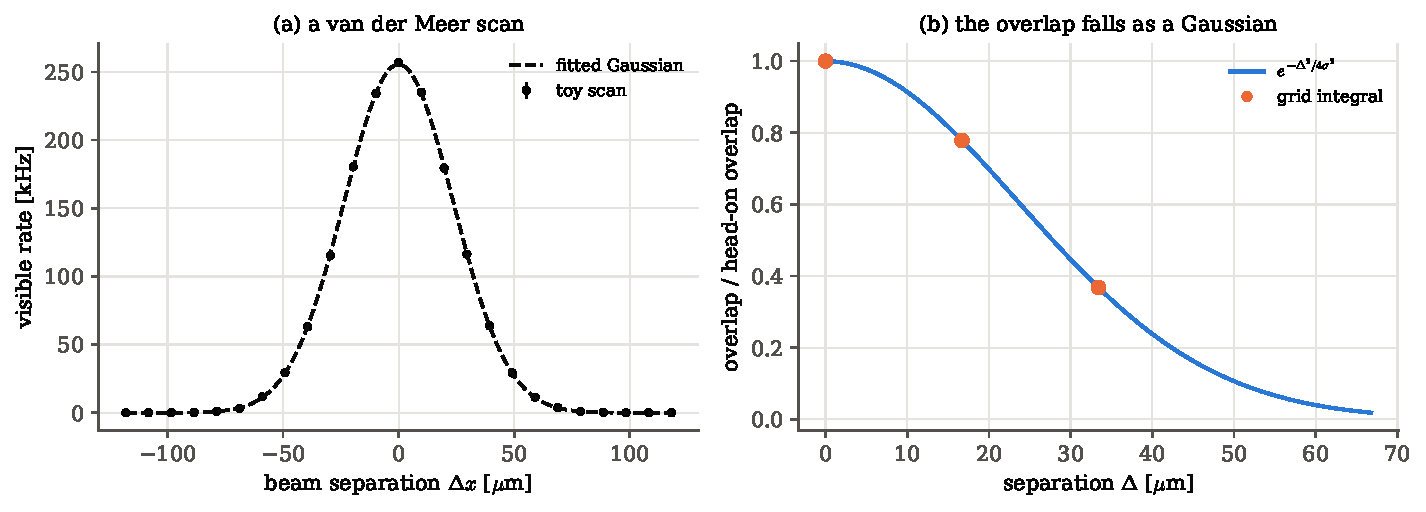
\includegraphics[width=\linewidth]{figures/chT4/vdm_scan.pdf}
\caption{(a) A toy van der Meer scan: the collision rate seen by a luminosity detector as one beam is moved sideways across the other. The rate traces a Gaussian whose width is the combined size $\Sigma_x$ of the two beams, which is what the luminosity formula needs. (b) The overlap of two equal Gaussian bunches falls with their separation as $e^{-\Delta^2/4\sigma^2}$; the points are the overlap integral computed numerically.}
\label{T4a:fig:vdm}
\end{figure}

The toy's statistical precision, a tenth of a per cent, is far better than the luminosity uncertainties of $1.8\%$ and $3.6\%$ that ATLAS quoted for 2011 and 2012 \cite[Sec.~4.3]{AadHiggs2012}. The real uncertainty comes from what the toy leaves out: bunch profiles that are not exactly Gaussian or do not factorise into an $x$ part times a $y$ part, the calibration of the separation $\Delta$ itself, and the stability of the luminosity detector between the scan, done in special conditions, and months of ordinary running. The toy shows the principle; the systematics of the real calibration set the number.

\paragraph{The energy scale: the $Z$ boson as a standard candle.}
The $Z$ boson's mass is known to $2$\,MeV, and $Z\to e^+e^-$ decays are plentiful. Electrons and photons make nearly the same showers in the calorimeter. So the electron pairs measure the energy scale: if the reconstructed $m_{ee}$ peak sits at $(1+\delta)\,m_Z$, then by \eqref{T4a:eq:scale-shift} the electron energies are too large by the fraction $\delta$, and they are corrected by $1/(1+\delta)$. ATLAS derived such $\eta$-dependent corrections, of order $\pm1\%$, from $Z\to e^+e^-$ events, and calibrated the photon identification and isolation efficiencies on electrons from $Z$ decays and on photons radiated in $Z\to\ell^+\ell^-\gamma$ decays \cite[Secs.~5.1, 5.6]{AadHiggs2012}. What remains uncertain is the transfer from electrons to photons (the material in front of the calorimeter affects them differently), which is why the material description appears among the scale and resolution uncertainties.

\emph{How a calibration enters the search.} A calibration is a measurement with a result $a_k$ and an error $\sigma_k$. Its probability, read as a function of the true parameter $\theta_k$, is a likelihood factor that multiplies the likelihood of the search histogram \cite[(40.17)]{PDG2024}, \cite[Sec.~2.2]{Cranmer2015}. \Cref{4b:sec:nuisance-hep} writes this full likelihood \eqref{4b:eq:full-like} with Gaussian constraint terms \eqref{4b:eq:constraint}, and \cref{4b:sec:profile-hep} removes the nuisance parameters by profiling.

\begin{keyidea}[One source, one parameter, one calibration]
Each source of systematic uncertainty is a nuisance parameter $\alpha_k$, with $\alpha_k=0$ nominal and $\alpha_k=\pm1$ its one-standard-deviation variations. It can rescale templates (luminosity, efficiencies, cross sections), move or widen them (energy scale, resolution), or fake a signal (background function). Its value is constrained by an independent calibration measurement, whose likelihood multiplies that of the search.
\end{keyidea}

\paragraph{Where this is used.}
The nuisance parameters $\bm\theta=(\beta,\kappa,\delta)$ of \cref{4b:sec:nuisance-hep}, a background normalisation, a signal yield and an energy-scale shift, are three of the sources above in their simplest form; their constraint terms are the calibrations of this section. In the capstone (\cref{ch:13}), the selection script \pyname{code/ch13/31_hyy_select.py} reads the release's \pyname{photon_pt_syst} column (\cref{T4a:sec:opendata}) to size the energy-scale variation, and the spurious-signal test of \cref{13d:sec:spurious} sizes the uncertainty of the background function.
\section{The Higgs boson search of 2012}
\label{T4a:sec:higgs}

On 4 July 2012 the ATLAS and CMS collaborations reported, each with its own detector and its own analysis, an excess of events near $125$\,GeV that the background could hardly produce, and that looked like the decays of the Higgs boson \cite{AadHiggs2012,ChatrchyanHiggs2012}. Those two papers use every piece assembled so far: cross sections and luminosities, invariant masses of photon and lepton pairs, simulated signal templates, background functions fitted to sidebands, a signal strength, nuisance parameters with calibrations, and finally a local and a global significance. The diphoton part of the search is also the template for the capstone of \cref{ch:13}.

\subsection{Their question and their setup}
\label{T4a:sec:higgs-setup}

\emph{The question.} Is there a particle with the properties of the Standard Model Higgs boson, and if so, at what mass? By 2011 the earlier experiments and the first LHC data had excluded most masses below $600$\,GeV except a window between $114$ and $127$\,GeV, and both LHC experiments had seen excesses near $125$\,GeV of about three standard deviations \cite[Sec.~1]{AadHiggs2012}. Three standard deviations had come and gone before. The 2012 data were to settle it.

\emph{What the theory fixes.} For a given Higgs mass $m_H$, the Standard Model predicts everything else: how often the boson is made, and how often it decays into each final state. There are four main ways to make it at the LHC \cite[Sec.~3]{AadHiggs2012}, drawn in \cref{T4a:fig:production}.
\begin{itemize}[itemsep=1pt,leftmargin=1.2em]
  \item \emph{Gluon fusion} (ggF): two gluons make a Higgs boson through a loop of top quarks. About $88\%$ of the diphoton signal at $m_H=126.5$\,GeV.
  \item \emph{Vector-boson fusion} (VBF): two quarks each radiate a $W$ or $Z$, which fuse; the two quarks fly off as jets close to the beams. About $7\%$.
  \item \emph{Associated production} with a $W$ or $Z$ (WH, ZH): a quark and an antiquark make a heavy vector boson that radiates the Higgs boson. About $3\%$ and $2\%$.
  \item \emph{Production with a top-quark pair} ($t\bar tH$): about $0.5\%$.
\end{itemize}
These are the fractions ATLAS quotes for its diphoton signal \cite[Sec.~5.4]{AadHiggs2012}. The total cross section at $m_H=125$\,GeV was predicted to be $17.5$\,pb at $\sqrt s=7$\,TeV and $22.3$\,pb at $8$\,TeV \cite[Sec.~3]{AadHiggs2012}.

\begin{figure}[htbp]
\centering
\begin{tikzpicture}[scale=0.82,
  gl/.style={decorate,decoration={coil,aspect=0,segment length=4pt,amplitude=2pt},thick},
  fe/.style={thick,midarrow},
  bo/.style={decorate,decoration={snake,segment length=6pt,amplitude=1.5pt},thick},
  hi/.style={thick,dashed,fibreorange},
  lb/.style={font=\scriptsize}]
  \begin{scope}
    \draw[gl] (0,1.0) -- (1.0,0.6);
    \draw[gl] (0,-1.0) -- (1.0,-0.6);
    \draw[fe,formblue] (1.0,0.6) -- (1.0,-0.6);
    \draw[fe,formblue] (1.0,-0.6) -- (1.8,0);
    \draw[fe,formblue] (1.8,0) -- (1.0,0.6);
    \draw[hi] (1.8,0) -- (2.9,0);
    \node[lb,anchor=east] at (0,1.0) {$g$};
    \node[lb,anchor=east] at (0,-1.0) {$g$};
    \node[lb,formblue] at (1.55,0.55) {$t$};
    \node[lb,anchor=west,fibreorange] at (2.9,0) {$H$};
    \node[font=\small] at (1.4,-1.6) {(a) ggF, $88\%$};
  \end{scope}
  \begin{scope}[xshift=4.4cm]
    \draw[fe] (0,1.0) -- (1.0,0.7);
    \draw[fe] (1.0,0.7) -- (2.6,1.1);
    \draw[fe] (0,-1.0) -- (1.0,-0.7);
    \draw[fe] (1.0,-0.7) -- (2.6,-1.1);
    \draw[bo] (1.0,0.7) -- (1.4,0);
    \draw[bo] (1.0,-0.7) -- (1.4,0);
    \draw[hi] (1.4,0) -- (2.6,0);
    \node[lb,anchor=east] at (0,1.0) {$q$};
    \node[lb,anchor=east] at (0,-1.0) {$q$};
    \node[lb,anchor=west] at (2.6,1.1) {jet};
    \node[lb,anchor=west] at (2.6,-1.1) {jet};
    \node[lb,anchor=east] at (1.15,0.25) {$W,Z$};
    \node[lb,anchor=west,fibreorange] at (2.6,0) {$H$};
    \node[font=\small] at (1.4,-1.6) {(b) VBF, $7\%$};
  \end{scope}
  \begin{scope}[xshift=8.8cm]
    \draw[fe] (0,1.0) -- (0.9,0);
    \draw[fe] (0.9,0) -- (0,-1.0);
    \draw[bo] (0.9,0) -- (1.9,0);
    \draw[bo] (1.9,0) -- (2.8,-0.9);
    \draw[hi] (1.9,0) -- (2.8,0.9);
    \node[lb,anchor=east] at (0,1.0) {$q$};
    \node[lb,anchor=east] at (0,-1.0) {$\bar q$};
    \node[lb] at (1.4,0.3) {$W^*,Z^*$};
    \node[lb,anchor=west] at (2.8,-0.9) {$W,Z$};
    \node[lb,anchor=west,fibreorange] at (2.8,0.9) {$H$};
    \node[font=\small] at (1.4,-1.6) {(c) WH, ZH, $5\%$};
  \end{scope}
  \begin{scope}[xshift=13.0cm]
    \draw[hi] (0,0) -- (0.9,0);
    \draw[fe,formblue] (0.9,0) -- (1.6,0.6);
    \draw[fe,formblue] (1.6,0.6) -- (1.6,-0.6);
    \draw[fe,formblue] (1.6,-0.6) -- (0.9,0);
    \draw[bo] (1.6,0.6) -- (2.5,1.0);
    \draw[bo] (1.6,-0.6) -- (2.5,-1.0);
    \node[lb,anchor=east,fibreorange] at (0,0) {$H$};
    \node[lb,anchor=west] at (2.5,1.0) {$\gamma$};
    \node[lb,anchor=west] at (2.5,-1.0) {$\gamma$};
    \node[lb,formblue,anchor=west] at (1.65,0) {$t,W$};
    \node[font=\small] at (1.3,-1.6) {(d) $H\to\gamma\gamma$};
  \end{scope}
\end{tikzpicture}
\caption{How a Higgs boson is made at the LHC (a--c, with the share of each mode in the 2012 diphoton signal; $t\bar tH$, $0.5\%$, is not drawn) and how it decays to two photons (d). The Higgs boson couples to mass, so it couples neither to the massless gluons nor to the photons directly; both (a) and (d) go through a loop of heavy charged particles, which is why the diphoton branching fraction is only about two per mille.}
\label{T4a:fig:production}
\end{figure}

\emph{The channels.} A Higgs boson of $125$\,GeV decays mostly to $b\bar b$, but the LHC makes $b$-quark pairs by the billion. Two final states combine a small branching fraction with a clean signature and an excellent mass resolution \cite[Secs.~4--5]{AadHiggs2012}, \cite[Sec.~1]{ChatrchyanHiggs2012}:
\begin{itemize}[itemsep=1pt,leftmargin=1.2em]
  \item $H\to\gamma\gamma$: two isolated photons, $\sigma B=50$\,fb at $8$\,TeV, mass resolution $1.6$\,GeV (\cref{T4a:sec:resolution});
  \item $H\to ZZ^{(*)}\to4\ell$: two pairs of electrons or muons, one pair with the mass of a $Z$, $\sigma B=2.8$\,fb at $8$\,TeV, resolution $1.7$--$2.3$\,GeV.
\end{itemize}
The superscript $(*)$ says that one of the two $Z$ bosons is off its mass shell: $125$\,GeV is not enough to make two real $Z$ bosons of $91$\,GeV each. ATLAS added $H\to WW^{(*)}\to e\nu\mu\nu$, which has many more events but, with two neutrinos escaping, no peak in any mass. CMS also used $\tau\tau$ and $b\bar b$. The data sets were small by later standards; \cref{T4a:tab:higgs-setup} collects them.

\begin{table}[htbp]
\centering
\small
\begin{tabular}{lcc}
\toprule
 & ATLAS \cite{AadHiggs2012} & CMS \cite{ChatrchyanHiggs2012} \\
\midrule
data, $7$\,TeV (2011) & $4.6$--$4.8\,\mathrm{fb^{-1}}$ & $4.9$--$5.1\,\mathrm{fb^{-1}}$ \\
data, $8$\,TeV (2012) & $5.8$--$5.9\,\mathrm{fb^{-1}}$ & $5.0$--$5.3\,\mathrm{fb^{-1}}$ \\
channels & $\gamma\gamma$, $4\ell$, $WW$ (+ $b\bar b$, $\tau\tau$ at $7$\,TeV) & $\gamma\gamma$, $4\ell$, $WW$, $\tau\tau$, $b\bar b$ \\
pile-up per crossing & about $10$ ($7$\,TeV), $20$ ($8$\,TeV) & --- \\
$\gamma\gamma$ events, $100$--$160$\,GeV & $23\,788$ ($7$\,TeV), $35\,251$ ($8$\,TeV) & --- \\
\bottomrule
\end{tabular}
\caption{The data of the two discovery papers. The luminosity ranges reflect the different data-quality requirements of the channels.}
\label{T4a:tab:higgs-setup}
\end{table}

\subsection{Their expected counts, recomputed}
\label{T4a:sec:higgs-counts}

\emph{The key equation.} The expected number of selected signal events in each channel is \eqref{T4a:eq:nu}, $\nu_S=\sigma B\,L\,\varepsilon A$, with $\sigma B$ the predicted cross section times branching fraction, $L$ the integrated luminosity and $\varepsilon A$ the fraction of produced events that survive the selection (\cref{T4a:sec:eff}). Both papers quote all four numbers or enough of them to recompute the others. Doing so shows what a discovery with $10\,\mathrm{fb^{-1}}$ looked like in events.

\paragraph{Example: the diphoton channel at $8$\,TeV.}
ATLAS expected $N_S=110.5$ signal events in all categories together between $100$ and $160$\,GeV, from $\sigma B=50$\,fb and $L=5.9\,\mathrm{fb^{-1}}$ \cite[Table~4]{AadHiggs2012}. Then
\begin{align}
  \sigma B\,L&=50\,\mathrm{fb}\times5.9\,\mathrm{fb^{-1}}=295\ \text{produced},
  \qquad
  \varepsilon A\eqby{1}\frac{N_S}{\sigma BL}=\frac{110.5}{295}=0.375 .
  \label{T4a:eq:atlas-eff}
\end{align}
\begin{explain}
  \item Solve $N_S=\sigma BL\,\varepsilon A$ for the selection efficiency.
\end{explain}
ATLAS quotes an overall selection efficiency of ``about $40\%$'' \cite[Sec.~5.4]{AadHiggs2012}. The recomputed $37.5\%$ is a little lower because $N_S$ also includes the $2$--$5\%$ reduction of the gluon-fusion rate from interference (\cref{T4a:sec:weights}), and because ``about'' is about. The same selection kept $N_D=\num{35251}$ data events in the same $60$\,GeV range. The signal was $0.3\%$ of the selected events, concentrated in a few GeV.

\paragraph{Example: the four-lepton channel.}
The four-lepton signal is tiny: $\sigma B=2.2$\,fb at $7$\,TeV and $2.8$\,fb at $8$\,TeV \cite[Sec.~4]{AadHiggs2012}, so with $4.8$ and $5.8\,\mathrm{fb^{-1}}$
\begin{equation}
  \sigma BL=2.2\times4.8+2.8\times5.8=10.6+16.2=26.8\ \text{produced four-lepton decays}.
\end{equation}
In a window of $\pm5$\,GeV around $125$\,GeV ATLAS expected $5.3$ signal events ($2.09+2.29+0.90$ in the $4\mu$, mixed and $4e$ sub-channels), an efficiency of $5.3/26.8=20\%$, and $4.9$ background events, mostly non-resonant $ZZ^{(*)}$ production ($2.4$) and $Z$+jets and $t\bar t$ ($2.5$). It observed $13$ \cite[Table~3]{AadHiggs2012}.

The two channels sit at opposite ends of the counting problem. In the diphoton channel thousands of background events per GeV surround a signal of a few dozen per GeV; the background is measured by the sidebands to high precision, and the question is whether a bump of a few per cent is real. In the four-lepton channel the signal and background are comparable, $5.3$ against $4.9$, and the question is whether $13$ is too many for a Poisson count of mean $4.9$, the small-count $p$-value of \cref{4a:sec:poisson-p}. Both questions have the same structure, $\nu=\mu s+b$ (\cref{T4a:sec:mu}); only the regime differs.

\subsection{What could have produced the excess?}
\label{T4a:sec:higgs-excess}

\emph{What was seen.} Both experiments saw more events than the background predicted, near $126$\,GeV in ATLAS and $125$\,GeV in CMS, in both the diphoton and the four-lepton channel (\cref{T4a:fig:opendata-mgg} shows what such a spectrum looks like). \emph{What could have produced it?} Before any number, the candidates.

\emph{A fluctuation of the background at this mass.} Background events arrive as Poisson counts (\cref{T4a:sec:poisson}), and a count can be high by chance. The probability that the background alone gives an excess at least as large as the one observed, at the mass where it was observed, is the local $p$-value $p_0$. For the ATLAS combination it was $1.7\times10^{-9}$ at $m_H=126.5$\,GeV, a local significance of $5.9$ standard deviations once the uncertainties of the energy scales and resolutions were included ($6.0$ without them); the Standard Model Higgs boson was expected to give $4.9$ on average \cite[Sec.~9.2]{AadHiggs2012}. CMS found $5.0$ standard deviations at $125.5$\,GeV, where $5.8$ were expected \cite[Sec.~7.1]{ChatrchyanHiggs2012}.

\emph{A fluctuation anywhere in the search range.} The excess was not looked for at $126$\,GeV only; it could have appeared at any mass in the range searched, and a fluctuation somewhere is far more likely than a fluctuation at one fixed place. The global significance, discussed below, answers this version of the question: $5.1$ standard deviations for ATLAS over $110$--$600$\,GeV.

\emph{A background shape that bends.} If the smooth background function were wrong near $126$\,GeV, the fit would mistake the difference for signal. That possibility is the spurious signal of \cref{T4a:sec:bkg-data}; it was measured in simulation and included in the likelihood as an extra uncertainty \cite[Sec.~5.5]{AadHiggs2012}.

\emph{An artefact of one detector.} A calibration fault in the calorimeter could fake a diphoton bump. It could not also fake a four-lepton bump at the same mass, whose muons are measured by the tracker and the muon spectrometer. Nor could one detector's fault appear in the other experiment. The masses agree: $126.0\pm0.4\,(\text{stat})\pm0.4\,(\text{sys})$\,GeV from ATLAS \cite[Sec.~9.3]{AadHiggs2012} and $125.3\pm0.4\pm0.5$\,GeV from CMS \cite[Sec.~7]{ChatrchyanHiggs2012}, $0.7$\,GeV apart with a combined uncertainty of about $0.9$\,GeV.

\emph{A new particle.} If the excess is a Higgs boson, its size should match the prediction, $\mu=1$ in the notation of \eqref{T4a:eq:mu}. ATLAS measured $\hat\mu=1.4\pm0.3$ at $126$\,GeV and CMS $\hat\mu=0.87\pm0.23$, both compatible with one \cite[Sec.~9.3]{AadHiggs2012}, \cite[Sec.~7]{ChatrchyanHiggs2012}. Both papers add that a particle decaying to two photons cannot have spin one, and that decays to pairs of neutral vector bosons make it a neutral boson \cite[Sec.~10]{AadHiggs2012}, \cite[Sec.~7]{ChatrchyanHiggs2012}.

Taken one at a time, each candidate except the last was either made improbable by a number or ruled out by a cross-check. Both collaborations therefore wrote ``observation of a new particle''. The first two candidates are the statistical part of the argument; we look at them more closely.

\subsection{Local and global significance}
\label{T4a:sec:local-global}

\emph{From $p$ to $Z$.} Particle physicists quote a $p$-value as the number $Z$ of standard deviations a one-sided Gaussian tail would need to have the same probability, $p=1-\Phi(Z)$, with $\Phi$ the standard normal cumulative distribution (\cref{4a:sec:p-to-z}). Five standard deviations, $p=2.9\times10^{-7}$, is the conventional threshold for ``observation'' (\cref{4a:sec:why-five}). The table below gives the values used in this section.
\begin{center}
\footnotesize
\setlength{\tabcolsep}{3pt}
\begin{tabular}{lcccccccc}
\toprule
$Z$ & $3.28$ & $4.5$ & $4.6$ & $5.0$ & $5.1$ & $5.3$ & $5.9$ & $6.0$ \\
$p=1-\Phi(Z)$ & $5.2\times10^{-4}$ & $3.4\times10^{-6}$ & $2.1\times10^{-6}$ & $2.9\times10^{-7}$ & $1.7\times10^{-7}$ & $5.8\times10^{-8}$ & $1.8\times10^{-9}$ & $9.9\times10^{-10}$ \\
\bottomrule
\end{tabular}
\end{center}

\emph{Local and global.} The \newterm{local significance} answers: if there is only background, how probable is an excess at least this large \emph{at this mass}? The \newterm{global significance} answers: how probable is an excess at least this large \emph{anywhere in the range that was searched}? The second probability is larger, because the search effectively performs many tests, one for each place a peak could sit; this is the \newterm{look-elsewhere effect} \cite[\S40.3.2.2]{PDG2024}, \cite[Sec.~4]{ChatrchyanHiggs2012}. Their ratio, the trials factor, is roughly the number of independent places in the range. ATLAS states that it grows with the width of the searched mass range, with the significance of the excess, and with the sharpness of the peaks (a better mass resolution means narrower peaks and more independent places) \cite[Sec.~7]{AadHiggs2012}.

\paragraph{Example: the trials factors of 2012.}
Using the table above, the ratios of global to local $p$-values are:
\begin{itemize}[itemsep=1pt,leftmargin=1.2em]
  \item ATLAS, local $5.9$: global $5.1$ over $110$--$600$\,GeV, a trials factor $1.7\times10^{-7}/1.8\times10^{-9}=94$; global $5.3$ over $110$--$150$\,GeV, a trials factor $5.8\times10^{-8}/1.8\times10^{-9}=32$ \cite[Sec.~9.2]{AadHiggs2012}.
  \item CMS, local $5.0$: global $4.6$ over $115$--$130$\,GeV, a factor $7$; global $4.5$ over $110$--$145$\,GeV, a factor $12$ \cite[Sec.~7.1]{ChatrchyanHiggs2012}.
\end{itemize}
The pattern follows the ranges: for CMS, widening the window from $15$ to $35$\,GeV raised the trials factor from $7$ to $12$, and for ATLAS, widening it from $40$ to $490$\,GeV raised it from $32$ to $94$. The factors of the two experiments cannot be compared directly, because the trials factor also grows with the significance itself ($5.9$ for ATLAS, $5.0$ for CMS) and depends on each experiment's resolution. The range up to $600$\,GeV adds fewer places than its length suggests, because at high masses the peaks are wide (the $4\ell$ resolution and the natural width grow with mass, \cref{T4a:sec:bw}) and the $WW$ channel has no peak at all.

\paragraph{Recall: the toy scan of \cref{ch:04}.}
\Cref{4b:sec:scan} ran exactly this computation on simulated background-only spectra: sixty $1$\,GeV bins from $100$ to $160$\,GeV, a Gaussian peak of width $\FourBScSigM$\,GeV scanned over $105$--$155$\,GeV. There the biggest bump had a local significance of $\FourBScZloc$, which the global $p$-value of $\FourBScPglob$ turned into $\FourBScZglob$ standard deviations, a trials factor of $\FourBScTrials$. The ATLAS search over $110$--$150$\,GeV is the closest real counterpart: a range of $40$ against $50$\,GeV, peaks of comparable width, and a trials factor of $32$ against $31$. What is the same is the mechanism, many places for a fluctuation; what differs is the size of the excess. The toy bump was a fluctuation that the global correction rightly demoted; the 2012 excess survived it with more than five standard deviations, and the global significance, not the local one, is the number that justified the word ``observation''. How the global $p$-value is computed without millions of toy experiments is \cref{4b:sec:gross-vitells}.

\begin{figure}[htbp]
\centering
\begin{tikzpicture}[x=1.45cm,y=1cm]
  \draw[thick,->] (0,0) -- (0,6.6) node[above,font=\small] {$Z$};
  \foreach \z in {0,1,...,6} {
    \draw (0,\z) -- (-0.08,\z) node[left,font=\scriptsize] {$\z$};
  }
  \fill[tangentgreen!12] (0.05,5) rectangle (7.6,6.45);
  \node[font=\scriptsize,tangentgreen!50!black,anchor=east] at (7.55,6.2) {``observation'', $Z\ge5$};
  \draw[softgray,dashed] (0,5) -- (7.6,5);
  \draw[softgray,dashed] (0,3) -- (7.6,3);
  \node[font=\scriptsize,softgray,anchor=east] at (7.55,3.2) {``evidence'', $Z\ge3$};
  \def\tfcol#1#2#3#4{%
    \fill[formblue] (#1,#2) circle (2.4pt);
    \draw[bdryred,thick] (#1,#3) circle (2.4pt);
    \draw[->,thick,softgray,shorten >=3pt,shorten <=3pt] (#1,#2) -- (#1,#3);
    \node[font=\scriptsize,align=center,anchor=north] at (#1,-0.15) {#4};}
  \tfcol{0.8}{5.9}{5.1}{ATLAS\\ $110$--$600$}
  \tfcol{1.9}{5.9}{5.3}{ATLAS\\ $110$--$150$}
  \tfcol{3.0}{5.0}{4.6}{CMS\\ $115$--$130$}
  \tfcol{4.1}{5.0}{4.5}{CMS\\ $110$--$145$}
  \tfcol{5.6}{\FourBScZloc}{\FourBScZglob}{toy scan of\\ \cref{4b:sec:scan}}
  \fill[formblue] (6.6,1.6) circle (2.4pt); \node[font=\scriptsize,anchor=west] at (6.7,1.6) {local};
  \draw[bdryred,thick] (6.6,1.1) circle (2.4pt); \node[font=\scriptsize,anchor=west] at (6.7,1.1) {global};
\end{tikzpicture}
\caption{Local (filled) and global (open) significance of the largest excess, for the two 2012 searches with two search ranges each (in GeV), and for the simulated background-only scan of \cref{ch:04}. Looking in a wider range always lowers the significance. The 2012 excesses stayed near or above five standard deviations after the correction; the toy bump, three standard deviations locally, dropped to about two.}
\label{T4a:fig:significance}
\end{figure}

\subsection{From 2012 to the open data}
\label{T4a:sec:higgs-lesson}

The capstone (\cref{ch:13}) asks the 2012 diphoton question of the 2016 open data, with one channel instead of several. What carries over unchanged is the chain from collisions to expected counts: $\nu=\sigma BL\varepsilon A$ for the signal, a simulated template for its shape, a smooth function fitted to the sidebands for the background, $\mu$ for the size of the signal, nuisance parameters for the calibrations. What changes is the collision energy and so the cross section: the gluon-fusion $\sigma B(\gamma\gamma)$ stored in the open-data files is $\TfdXsecTree$\,pb $=102$\,fb at $13$\,TeV, twice the $50$\,fb of \emph{all} production modes together at $8$\,TeV. With $10\,\mathrm{fb^{-1}}$ the open data therefore contain more Higgs bosons decaying to two photons than the whole 2012 diphoton sample of ATLAS. They also contain more background, and the open data were not processed with the full analysis machinery of the collaboration. Whether the bump appears, and how strongly, is the subject of \cref{ch:13}.

\emph{The lesson in one line.} A discovery is a chain of physical predictions, each with its calibration, ending in one comparison of counts; the statistics can only be as good as the expected counts $\nu_i$ it is given.
\section{The open data: what is in the files}
\label{T4a:sec:opendata}

In 2020 ATLAS released to the public a part of the proton collisions it recorded at $\sqrt s=13$\,TeV in 2016, together with simulated events for the main Standard Model processes \cite{ATLASOpenData2020,SerkinOpenData2020}. The capstone of \cref{ch:13} analyses its diphoton part. The files are not the raw detector output: they are tables with one row per recorded event and one column per reconstructed quantity, the reconstructed objects of \cref{T4a:sec:events} written out as numbers. Everything this chapter has introduced has a column, or a combination of columns, in these tables. Reading the columns correctly is the last physical step before the statistics.

\emph{The questions.} What exactly is in a row? Which column is which quantity of this chapter, and in what units? And what does a real event look like when we compute its invariant mass by hand?

\subsection{The release}
\label{T4a:sec:release}

The recorded events come from the first four data-taking periods of 2016, about $270$ million collisions written to disk. Only events taken while all relevant parts of the detector were working are kept, and after these quality requirements the data correspond to an integrated luminosity of $L=10\,\mathrm{fb^{-1}}$ \cite[Sec.~2]{SerkinOpenData2020}. The format is a ROOT tree, a column-oriented table, with more than $80$ columns (\newterm{branches}) \cite[Sec.~2]{SerkinOpenData2020}. The overview of the release lists the photon requirements as reconstruction in the inner detector and electromagnetic calorimeter, $E_T>25$\,GeV, $\lvert\eta\rvert<2.37$, tight identification and loose isolation \cite[Table~1]{SerkinOpenData2020}. The diphoton files nevertheless keep candidates that fail the tight identification and record the result in a flag: requiring the flag on both photons keeps only $\tfouraN{\TfdFlowDD}$ of the $\tfouraN{\TfdFlowDA}$ data events (\cref{T4a:fig:cutflow}). The flag must be checked.

The release is split into collections by final state. The diphoton collection, \texttt{GamGam}, holds four data files, one per period (A to D), and simulated Higgs bosons with $m_H=125$\,GeV decaying to two photons, one file per production mode (gluon fusion, vector-boson fusion, $WH$, $ZH$). It contains only events that passed a two-photon trigger and have two photon candidates. In all four data files the script \pyname{02_open_data.py} finds $\tfouraN{\TfdNtot}$ events, every one of them with the photon trigger flag set and exactly two photon candidates stored (\cref{T4a:fig:opendata-cols}d). The first two lines of the cut flow of \cref{T4a:fig:cutflow} therefore remove nothing: the release had already applied them.

\emph{Recall: the luminosity of the release.} \Cref{T4a:sec:xsec} used $L=10\,\mathrm{fb^{-1}}$ to predict $\TfdNprod$ produced and $\TfdNexp$ selected gluon-fusion Higgs decays. The capstone uses $L=10.06\,\mathrm{fb^{-1}}$ (\cref{13d:sec:data}), the value the release's own analysis code multiplies by, of which the published ``$10\,\mathrm{fb^{-1}}$'' is the rounded form. The two differ by $0.6\%$, a sixth of the $3.6\%$ luminosity uncertainty of the 2012 data (\cref{T4a:sec:calib}); every expected count in this chapter would be $0.6\%$ larger with the capstone's value.

\subsection{The columns}
\label{T4a:sec:columns}

A row of the diphoton tree has three kinds of column (\cref{T4a:fig:row}). \emph{Event-level numbers} describe the whole crossing: which run and event it is, which trigger fired, and for simulated events the weights. \emph{Per-object vectors} hold one entry per reconstructed photon (or lepton, or jet): \pyname{photon_pt} is a list of transverse momenta, the first entry for the leading photon, the second for the next. \emph{Normalisation constants} of the simulation, $\sigma B$ and the total weight $W$ of \eqref{T4a:eq:mc-norm}, are stored in every row of a simulated file. \Cref{T4a:tab:columns} lists the columns a diphoton analysis uses; the full list of the tree is written by the script to \pyname{results/chT4/02_branches.txt}.

\begin{figure}[htbp]
\centering
\begin{tikzpicture}[
  cell/.style={draw=softgray,font=\scriptsize\ttfamily,minimum height=0.55cm,inner sep=2pt,anchor=west},
  grp/.style={font=\small\bfseries,anchor=west}]
  \node[grp,accent] at (0,0.95) {event-level};
  \node[cell,minimum width=2.5cm] at (0,0) {runNumber};
  \node[cell,minimum width=2.5cm] at (0,-0.55) {eventNumber};
  \node[cell,minimum width=2.5cm] at (0,-1.1) {trigP = true};
  \node[cell,minimum width=2.5cm] at (0,-1.65) {photon\_n = 2};
  \node[grp,formblue] at (2.9,0.95) {one entry per photon};
  \node[cell,minimum width=2.9cm] at (2.9,0) {photon\_pt};
  \node[cell,minimum width=1.4cm,fill=formblue!8] at (5.9,0) {$\TfdPtA$};
  \node[cell,minimum width=1.4cm,fill=formblue!8] at (7.3,0) {$\TfdPtB$};
  \node[cell,minimum width=2.9cm] at (2.9,-0.55) {photon\_eta};
  \node[cell,minimum width=1.4cm,fill=formblue!8] at (5.9,-0.55) {$\tfouraR{3}{\TfdEtaA}$};
  \node[cell,minimum width=1.4cm,fill=formblue!8] at (7.3,-0.55) {$\tfouraR{3}{\TfdEtaB}$};
  \node[cell,minimum width=2.9cm] at (2.9,-1.1) {photon\_phi};
  \node[cell,minimum width=1.4cm,fill=formblue!8] at (5.9,-1.1) {$\tfouraR{3}{\TfdPhiA}$};
  \node[cell,minimum width=1.4cm,fill=formblue!8] at (7.3,-1.1) {$\tfouraR{3}{\TfdPhiB}$};
  \node[cell,minimum width=2.9cm] at (2.9,-1.65) {photon\_E};
  \node[cell,minimum width=1.4cm,fill=formblue!8] at (5.9,-1.65) {$\TfdEA$};
  \node[cell,minimum width=1.4cm,fill=formblue!8] at (7.3,-1.65) {$\TfdEB$};
  \node[cell,minimum width=2.9cm] at (2.9,-2.2) {photon\_isTightID};
  \node[cell,minimum width=1.4cm,fill=formblue!8] at (5.9,-2.2) {true};
  \node[cell,minimum width=1.4cm,fill=formblue!8] at (7.3,-2.2) {true};
  \node[font=\scriptsize,formblue] at (6.65,0.45) {$\gamma_1$};
  \node[font=\scriptsize,formblue] at (8.05,0.45) {$\gamma_2$};
  \node[grp,fibreorange] at (9.0,0.95) {simulation only};
  \node[cell,minimum width=2.7cm] at (9.0,0) {mcWeight};
  \node[cell,minimum width=2.7cm] at (9.0,-0.55) {scaleFactor\_*};
  \node[cell,minimum width=2.7cm] at (9.0,-1.1) {XSection};
  \node[cell,minimum width=2.7cm] at (9.0,-1.65) {SumWeights};
  \node[cell,minimum width=2.7cm] at (9.0,-2.2) {photon\_pt\_syst};
\end{tikzpicture}
\caption{The anatomy of one row of the diphoton tree. Left: numbers that describe the whole event. Middle: vectors with one entry per photon candidate, here filled with the first selected data event (momenta and energies in GeV after dividing the stored MeV by $1000$). Right: columns that are meaningful only for simulated events: the weights and the normalisation of \eqref{T4a:eq:mc-norm}, and the energy-scale variation of each photon.}
\label{T4a:fig:row}
\end{figure}

\begin{table}[htbp]
\centering
\small
\begin{tabularx}{\linewidth}{>{\raggedright\arraybackslash\ttfamily}p{3.6cm} >{\raggedright\arraybackslash}X >{\raggedright\arraybackslash}p{2.9cm}}
\toprule
\normalfont column & meaning & symbol, section \\
\midrule
runNumber, eventNumber & which data-taking run and which crossing & --- \\
trigP & the photon trigger fired & \cref{T4a:sec:events} \\
photon\_n & number of photon candidates stored & --- \\
photon\_pt & transverse momentum, MeV & $p_T$, \eqref{T4a:eq:pt} \\
photon\_eta & pseudorapidity $-\ln\tan(\theta/2)$ & $\eta$, \eqref{T4a:eq:eta} \\
photon\_phi & azimuth around the beam, rad & $\phi$, \cref{T4a:sec:coordinates} \\
photon\_E & energy, MeV & $E=p_T\cosh\eta$ \\
photon\_isTightID & shower shape passes the tight photon identification & $\varepsilon$, \cref{T4a:sec:eff} \\
photon\_etcone20 & calorimeter transverse energy in a cone $\Delta R<0.2$ around the photon, MeV & isolation \\
photon\_ptcone30 & sum of track $p_T$ in a cone $\Delta R<0.3$, MeV & isolation \\
photon\_convType & $0$ if unconverted, otherwise how it converted to $e^+e^-$ & categories \\
photon\_pt\_syst & energy-scale variation of the photon's $p_T$, MeV (simulation) & $\delta$, \eqref{T4a:eq:scale-shift} \\
mcWeight & generator weight of the event & $w_e$, \eqref{T4a:eq:mc-norm} \\
scaleFactor\_* & data/simulation corrections of the photon efficiency (\texttt{\_PHOTON}), the trigger efficiency (\texttt{\_PhotonTRIGGER}) and the pile-up (\texttt{\_PILEUP}) & factors of $w_e$ \\
XSection & cross section times branching fraction, pb & $\sigma B$ \\
SumWeights & sum of the weights of all generated events & $W$, \eqref{T4a:eq:mc-norm} \\
\bottomrule
\end{tabularx}
\caption{The columns a diphoton analysis reads, their meaning, and the symbol each carries. Momenta and energies are stored in MeV. The cone size $\Delta R=\sqrt{\Delta\eta^2+\Delta\phi^2}$ is a distance in the $(\eta,\phi)$ plane.}
\label{T4a:tab:columns}
\end{table}

Four columns need a word beyond the table.
\begin{itemize}[itemsep=1pt,leftmargin=1.2em]
  \item \emph{Isolation.} \pyname{photon_etcone20} adds up the transverse energy deposited in the calorimeter in a cone of radius $\Delta R=0.2$ around the photon, excluding the photon's own shower. A photon from a Higgs decay is alone, so this sum is small; a ``photon'' that is really a neutral pion inside a jet is surrounded by the jet's other hadrons. Requiring less than $4$\,GeV, as ATLAS did in 2012 \cite[Sec.~5.1]{AadHiggs2012}, keeps $\tfouraR{1}{\TfdIsoMC}\%$ of simulated signal photons and only $\tfouraR{1}{\TfdIsoData}\%$ of the photon candidates in the data (\cref{T4a:fig:opendata-cols}c).
  \item \emph{Conversion.} A photon crossing the inner detector may convert into an electron--positron pair before it reaches the calorimeter; its energy is then measured less well and its shower starts earlier. Of the selected photons in the data, $\tfouraR{1}{\TfdConv}\%$ are converted. The 2012 analysis split events into categories by conversion status because the resolution differs (\cref{T4a:sec:higgs-counts}); the capstone uses the unconverted central category the same way.
  \item \emph{Scale factors.} The simulation reproduces efficiencies only approximately. Each factor is the ratio of an efficiency measured in data (for example with photons from $Z\to\ell^+\ell^-\gamma$, \cref{T4a:sec:calib}) to the same efficiency in simulation, and multiplies the event's weight. The product $w_e=\texttt{mcWeight}\times\prod\texttt{scaleFactor}$ is the weight of \eqref{T4a:eq:mc-norm}.
  \item \emph{The energy-scale variation.} \pyname{photon_pt_syst} gives, for each simulated photon, how far its $p_T$ moves when the energy scale is varied by its uncertainty. Its median relative size in the selected signal is $\tfouraR{2}{\TfdSystRel}\%$. By \eqref{T4a:eq:scale-shift} this is directly the relative shift of the diphoton peak, the energy-scale nuisance parameter of \cref{T4a:sec:sources}. In the data files the column carries no information, as it must: a recorded energy has no ``varied'' version.
\end{itemize}

\begin{pitfall}[The files store MeV]
Momenta and energies in the 2016 release are in MeV, not GeV. An invariant mass computed without dividing by $1000$ comes out near $125\,000$, and a cut ``$p_T>40$'' applied to the raw column keeps every photon. The script checks the median $p_T$ and divides by $1000$ when it is above a thousand.
\end{pitfall}

\subsection{One event by hand}
\label{T4a:sec:first-event}

\emph{The question.} Take the first event of period A that passes the selection of \cref{T4a:sec:eff}. What is its diphoton mass, and do the columns agree with each other?

The two photons have, after conversion to GeV, $p_{T1}=\TfdPtA$ and $p_{T2}=\TfdPtB$\,GeV, $\eta_1=\tfouraR{4}{\TfdEtaA}$ and $\eta_2=\tfouraR{4}{\TfdEtaB}$, $\phi_1=\tfouraR{4}{\TfdPhiA}$ and $\phi_2=\tfouraR{4}{\TfdPhiB}$\,rad, and energies $E_1=\TfdEA$ and $E_2=\TfdEB$\,GeV.

\emph{Check one: are the energies those of massless particles?} For a photon, $E=\lvert\bm p\rvert=p_T\cosh\eta$ \eqref{T4a:eq:eta-identities}. With $\cosh(0.8335)=1.368$ and $\cosh(0.0947)=1.0045$, $176.1\times1.368=240.9$ and $39.63\times1.0045=39.81$\,GeV: both stored energies are reproduced to the last digit. The columns are consistent, and the photons are massless as they should be.

\emph{The mass from the detector variables.} With \eqref{T4a:eq:mgg}, $\Delta\eta=\eta_1-\eta_2=-0.9282$ and $\Delta\phi=\phi_1-\phi_2=-0.8615$,
\begin{align}
  m_{\gamma\gamma}^2
  &\eqby{1}2\,p_{T1}p_{T2}\bigl(\cosh\Delta\eta-\cos\Delta\phi\bigr)
  \eqby{2}2\times176.1\times39.63\times(1.4626-0.6513)
  \nonumber\\
  &\eqby{3}\num{13958}\times0.8113=\num{11324}\,\mathrm{GeV^2},
  \qquad
  m_{\gamma\gamma}=106.4\,\mathrm{GeV}.
  \label{T4a:eq:first-event}
\end{align}
\begin{explain}
  \item The diphoton mass in detector variables, \eqref{T4a:eq:mgg}.
  \item $\cosh(-0.9282)=\cosh(0.9282)=1.4626$ (cosh is even) and $\cos(-0.8615)=0.6513$.
  \item Multiply out.
\end{explain}
\emph{The mass from four-vectors.} Build $p_x=p_T\cos\phi$, $p_y=p_T\sin\phi$, $p_z=p_T\sinh\eta$ for each photon and add: the pair has $\bm P=(202.0,\,-29.8,\,-160.6)$\,GeV and $E=280.7$\,GeV, so $m^2=E^2-\lvert\bm P\rvert^2$ by \eqref{T4a:eq:minv-general} gives $m=106.4$\,GeV again. The script finds $\TfdMfirst$ and $\TfdMvec$\,GeV for the two routes.

This event is not a Higgs boson candidate in any useful sense: its mass is $19$\,GeV below the peak, and in any case a single event is neither signal nor background (\cref{13d:sec:data}). It is a typical background event. The pair is strongly boosted along the beam, $P_z=-161$\,GeV, which is the unknown parton motion of \cref{T4a:sec:coordinates}; the mass does not care.

\subsection{What the columns look like}
\label{T4a:sec:column-plots}

\Cref{T4a:fig:opendata-cols} histograms four columns for the data and for the simulated gluon-fusion signal, after the trigger and two-photon requirement and before any other cut.

\begin{figure}[htbp]
\centering
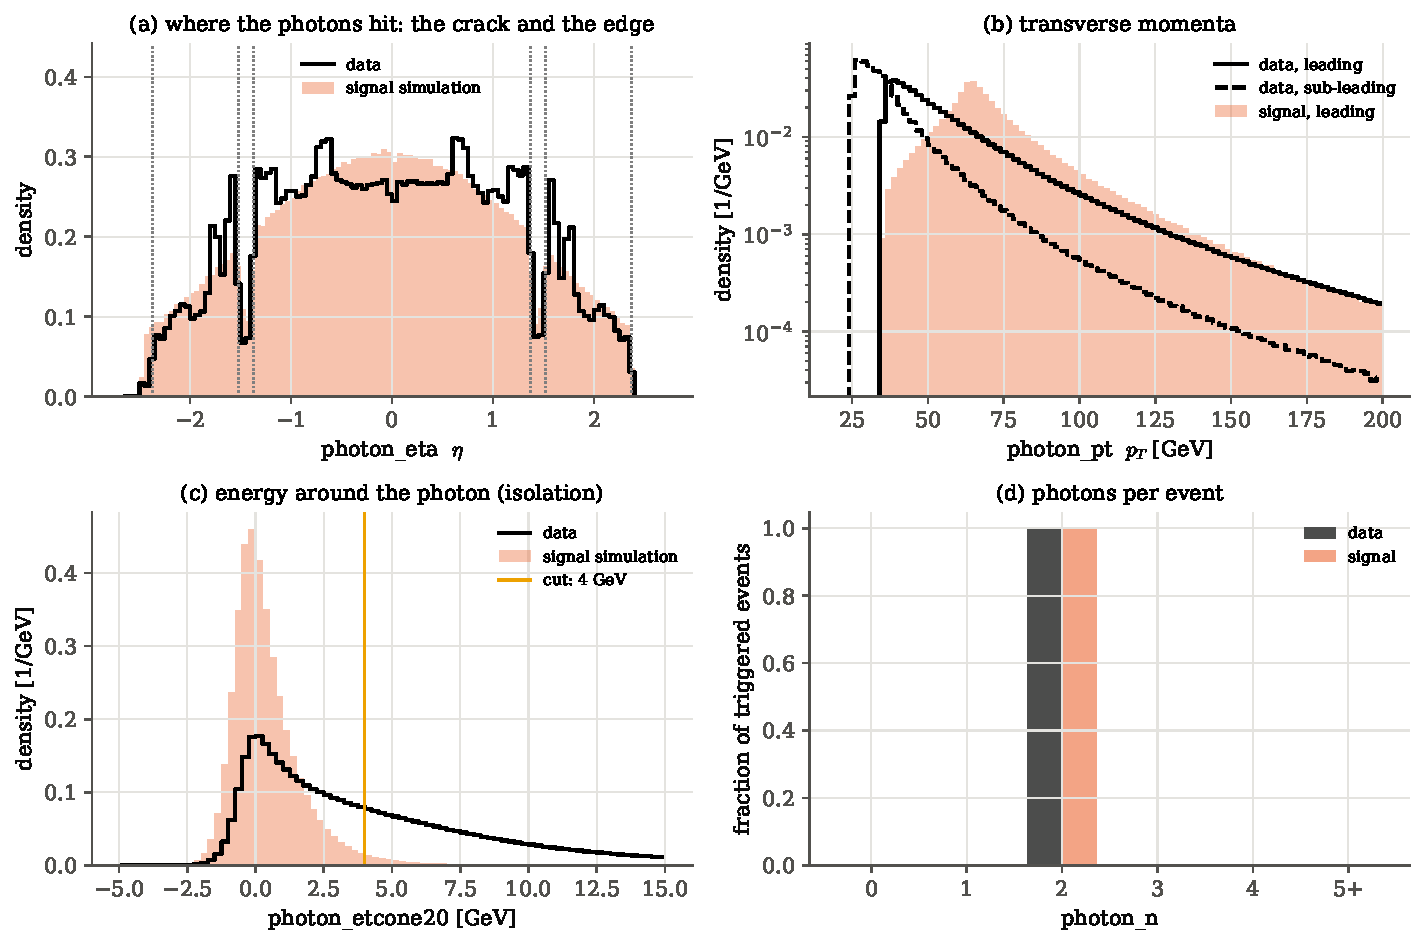
\includegraphics[width=\linewidth]{figures/chT4/opendata_columns.pdf}
\caption{Four columns of the diphoton files, for recorded events (black) and simulated Higgs decays (filled). (a) Photon pseudorapidity: no photon beyond the calorimeter edge at $\lvert\eta\rvert=2.37$, and a dip in the data at the barrel/end-cap gap $1.37<\lvert\eta\rvert<1.52$ (dotted lines). (b) Transverse momenta: the data fall steeply from the trigger thresholds, while the signal photons peak near half the Higgs mass. (c) Isolation energy: signal photons are alone, with a narrow peak near zero; the data have a long tail from jets faking photons, which the $4$\,GeV cut removes. (d) Every event in the files has exactly two photon candidates.}
\label{T4a:fig:opendata-cols}
\end{figure}

\paragraph{Example: reading the pseudorapidity panel.}
In panel (a) the signal photons spread smoothly over the calorimeter, more of them at small $\lvert\eta\rvert$, because the decay products of a Higgs boson with modest longitudinal motion come out at all angles. The data have structure the signal lacks: the density of data candidates changes abruptly at the boundaries of the calorimeter regions, while the simulated signal, made of real photons, changes smoothly. The data are mostly fake photons from jets, and how often a jet passes as a photon depends on the calorimeter region. Of the data photon candidates, $\tfouraR{1}{\TfdCrack}\%$ sit inside the gap $1.37<\lvert\eta\rvert<1.52$, where the energy measurement is poor; the selection removes them. This is the acceptance cut of \cref{T4a:sec:eff} seen in the raw columns.

\paragraph{Example: reading the momentum panel.}
In panel (b) the data start at the trigger and preselection thresholds, about $35$\,GeV for the leading and $25$\,GeV for the second photon, and fall over three orders of magnitude by $200$\,GeV. The signal's leading photon peaks near $m_H/2=62.5$\,GeV, the energy of a photon from a Higgs boson at rest (\cref{T4a:sec:minv}), with a tail to higher values from the boost. Cuts on $p_T$ therefore remove much of the low-mass background while keeping most of the signal; the capstone uses cuts relative to $m_{\gamma\gamma}$ instead, for the reason given in \cref{13d:sec:data}.

\paragraph{Recall: this selection and the capstone's.}
\Cref{T4a:sec:eff} followed the gluon-fusion signal through a selection modelled on the 2012 analysis: tight identification, $\lvert\eta\rvert<2.37$ outside the gap, $p_T>40$ and $30$\,GeV, calorimeter isolation below $4$\,GeV, and $100<m_{\gamma\gamma}<160$\,GeV. It kept $\tfouraN{\TfdNsel}$ data events and $\TfdNexp$ expected signal events. The capstone (\cref{13d:sec:data}) uses the selection of the release's own example analysis: exactly two photons each passing tight identification with $p_T>25$\,GeV, both a calorimeter and a track isolation below $6.5\%$ of the photon's $p_T$, the relative cuts $p_{T1}/m_{\gamma\gamma}>0.35$ and $p_{T2}/m_{\gamma\gamma}>0.25$, and $105<m_{\gamma\gamma}<160$\,GeV. It keeps $\tfouraN{\HyyNData}$ data events and $\HyySigggH$ gluon-fusion events ($\HyySigExp$ from all four production modes). The capstone's data sample is half as large as ours and its gluon-fusion signal $10\%$ smaller: the extra track isolation and the relative isolation cut remove many more jets than signal photons, and the narrower mass range removes $5$\,GeV of the steepest part of the background. If the background under the peak falls in the same proportion as the whole sample, $s/\sqrt b$ in a fixed window grows by $0.9/\sqrt{0.5}\approx1.3$, which is the purpose of the tighter selection; \cref{13d:sec:data} shows its cut flow.

\paragraph{Where this is used.}
The capstone reads exactly the columns of \cref{T4a:tab:columns}: the photon momenta for $m_{\gamma\gamma}$ via \eqref{T4a:eq:mgg}, the identification, isolation and conversion flags for the selection and the categories, and \pyname{mcWeight}, the scale factors, \pyname{XSection} and \pyname{SumWeights} for the signal template \eqref{T4a:eq:mc-norm}.
\section{The symbols of a collider search}
\label{T4a:sec:symbols}

The statistics of a search treats each quantity of a collider measurement as a given number or function. \Cref{T4a:tab:symbols} lists each one with its meaning, the relation that defines or computes it, a typical size for the diphoton search, and the places where it is used. Two symbols are easily confused and are kept apart throughout the book: $\mu$ is always the signal strength, never a mean; the mean number of events is always $\nu$. The integrated luminosity is $L$ and the likelihood is $\Like$; HistFactory and Cranmer write $\lambda$ for the luminosity for the same reason.

\begin{small}
\setlength{\tabcolsep}{4pt}
\begin{xltabular}{\linewidth}{>{\raggedright\arraybackslash}p{1.5cm} >{\raggedright\arraybackslash}X >{\raggedright\arraybackslash}p{3.6cm} >{\raggedright\arraybackslash}p{2.6cm} >{\raggedright\arraybackslash}p{2.0cm}}
\caption{The symbols of a collider search: meaning, working relation, typical size in the diphoton search, and where each is used.}
\label{T4a:tab:symbols}\\
\toprule
symbol & meaning & working relation & typical size & used in \\
\midrule
\endfirsthead
\toprule
symbol & meaning & working relation & typical size & used in \\
\midrule
\endhead
\bottomrule
\endfoot
$\sqrt s$ & collision energy of the two protons & --- & $7$, $8$, $13$\,TeV & \cref{T4a:sec:higgs,ch:13} \\
$p_T$ & momentum transverse to the beam & $\lvert\bm p\rvert\sin\theta$, \eqref{T4a:eq:pt} & $25$--$200$\,GeV & \cref{T4a:sec:opendata,ch:13} \\
$y$ & rapidity; shifts by a constant under a boost along the beam & $\frac12\ln\frac{E+p_z}{E-p_z}$, \eqref{T4a:eq:rapidity} & --- & \cref{T4a:sec:coordinates} \\
$\eta$ & pseudorapidity, a measure of the polar angle & $-\ln\tan\frac\theta2$, \eqref{T4a:eq:eta} & $\lvert\eta\rvert<2.37$ & \cref{T4a:sec:opendata,ch:13} \\
$\phi$ & azimuth around the beam & --- & $(-\pi,\pi]$ & \cref{ch:13} \\
$\sigma$ & cross section of a process & $N=\sigma L$ & $\sigma_{\rm inel}=78$\,mb; $\sigma B=0.102$\,pb & \cref{T4a:sec:xsec,ch:13} \\
$L_{\rm inst}$ & instantaneous luminosity & $\dfrac{n_bfN_1N_2}{4\pi\sigma_x\sigma_y}F$, \eqref{T4a:eq:lumi} & $10^{34}\,\mathrm{cm^{-2}s^{-1}}$ & \cref{T4a:sec:lumi} \\
$L$ & integrated luminosity & $\int L_{\rm inst}\,\dd t$ & $10\,\mathrm{fb^{-1}}$ & \cref{4b:sec:templates,ch:13} \\
$\bar n_{\rm pu}$ & collisions per bunch crossing (pile-up) & $\sigma_{\rm inel}L_{\rm inst}/n_bf$, \eqref{T4a:eq:pileup} & $20$--$50$ & \cref{T4a:sec:lumi} \\
$A$, $\varepsilon$ & acceptance, efficiency & fraction of produced events kept & $\varepsilon A=0.39$ & \cref{T4a:sec:eff,ch:13} \\
$\nu$ & expected number of selected events & $\sigma L\varepsilon A$, \eqref{T4a:eq:nu}; Poisson mean & $395$ signal & \cref{4b:sec:binned-like} \\
$m_{\gamma\gamma}$ & invariant mass of the photon pair & $m^2=2p_{T1}p_{T2}\,\times$ $(\cosh\Delta\eta-\cos\Delta\phi)$, \eqref{T4a:eq:mgg} & $100$--$160$\,GeV & \cref{4b:sec:scan,ch:13} \\
$\Gamma$, $\tau$ & natural width, lifetime & $\Gamma=\hbar/\tau$; Breit--Wigner \eqref{T4a:eq:bw} & $\Gamma_H=4$\,MeV, $\Gamma_Z=2.5$\,GeV & \cref{T4a:sec:bw} \\
$\sigma_E/E$ & calorimeter energy resolution & $a/\sqrt E\oplus c$, \eqref{T4a:eq:eres} & $1.4\%$ at $62.5$\,GeV & \cref{T4a:sec:resolution} \\
$\sigma_m$ & mass resolution & $\frac12\sqrt{\sum(\sigma_{E_j}/E_j)^2}\,m$, \eqref{T4a:eq:mres} & $1.2$--$1.6$\,GeV & \cref{4b:sec:scan,ch:13} \\
$\alpha$, $n$ & Crystal Ball tail start and power & \eqref{T4a:eq:cb}, \eqref{T4a:eq:cb-AB} & $1.5$, $5$ & \cref{13d:sec:signal-shape} \\
$s_i$, $b_i$ & signal and background templates in bin $i$ & $s_i=\sum_{e\in i}\sigma Lw_e/W$, \eqref{T4a:eq:mc-norm}; $b_i$ from sidebands & $\sum s_i\approx400$ & \cref{4b:sec:templates,13d:sec:shapes} \\
$w_e$, $W$ & weight of a simulated event, total weight & \texttt{mcWeight}$\times$scale factors; \texttt{SumWeights} & $W=5.6\times10^7$ & \cref{T4a:sec:weights} \\
$\mu$ & signal strength & $\sigma B/(\sigma B)_{\rm SM}$; $\nu_i=\mu s_i+b_i$, \eqref{T4a:eq:mu} & $1.4\pm0.3$ (ATLAS 2012) & \cref{4b:sec:templates,4b:sec:limits} \\
$\alpha_k$ & nuisance parameter of source $k$ & $0$ nominal, $\pm1$ one s.d.; \eqref{T4a:eq:interp} & --- & \cref{4b:sec:nuisance-hep} \\
$\delta$ & energy-scale shift & $\delta m/m=\delta$, \eqref{T4a:eq:scale-shift} & $0.3\%$ & \cref{4b:sec:nuisance-hep} \\
$\Sigma_x$ & combined width of two beams & $\sqrt{s_1^2+s_2^2}$, \eqref{T4a:eq:vdm} & $24\,\mu$m & \cref{T4a:sec:calib} \\
$\sigma_{\rm vis}$ & visible cross section of a luminosity detector & $R_0/L_0$ & tens of mb & \cref{T4a:sec:calib} \\
$Z$, $p_0$ & significance, background-only $p$-value & $p_0=1-\Phi(Z)$ & $5.9$, $1.7\times10^{-9}$ & \cref{4a:sec:p-to-z,4b:sec:lee} \\
\end{xltabular}
\end{small}

\begin{recap}
\begin{itemize}[itemsep=1pt,leftmargin=1.2em]
  \item An event is a list of reconstructed particles, each with $p_T$, $\eta$, $\phi$; the transverse plane and rapidity differences are used because the motion of the colliding partons along the beam is unknown.
  \item With the integrated luminosity fixed, the number of selected events of a process is Poisson with mean $\nu=\sigma L\varepsilon A$.
  \item The invariant mass of a decay's products equals the parent's mass in every event; the peak's width combines the natural width (Breit--Wigner) and the detector resolution (Gaussian or Crystal Ball core), and is dominated by the larger.
  \item The expected count in a bin is $\nu_i=\mu s_i+b_i$: signal templates from weighted simulation, background from the sidebands of the data, $\mu=\sigma B/(\sigma B)_{\rm SM}$.
  \item Every uncertain input is a nuisance parameter with its own calibration: van der Meer scans for the luminosity, $Z$ decays for energy scale and efficiencies, simulated background samples for the spurious signal.
  \item In 2012 ATLAS saw a local $5.9\sigma$ and a global $5.1\sigma$ excess at $126$\,GeV, CMS a local $5.0\sigma$ at $125.5$\,GeV, with $\hat\mu=1.4\pm0.3$ and $0.87\pm0.23$.
  \item The 2016 open data store, per event, the photon four-momenta in MeV, identification, isolation and conversion flags, and for simulation the weights, scale factors, $\sigma B$ and the total weight.
\end{itemize}
\end{recap}

\section*{Chapter summary}
\addcontentsline{toc}{section}{Chapter summary}
\label{T4a:sec:summary}

\begin{small}
\setlength{\tabcolsep}{4pt}
\begin{xltabular}{\linewidth}{>{\raggedright\arraybackslash}p{3.0cm} >{\raggedright\arraybackslash}X >{\raggedright\arraybackslash}p{3.4cm}}
\toprule
concept & operational meaning & used later in \\
\midrule
\endfirsthead
\toprule
concept & operational meaning & used later in \\
\midrule
\endhead
\bottomrule
\endfoot
event, reconstructed object & one bunch crossing kept by the trigger, written as a list of photons, leptons, jets with $(p_T,\eta,\phi,E)$ & \cref{ch:13} (the data rows) \\
transverse plane, pseudorapidity & coordinates insensitive to the unknown parton motion along the beam; $\eta=-\ln\tan(\theta/2)$ & \cref{ch:13} (acceptance cuts) \\
cross section, luminosity & $N=\sigma L$: the process's effective area times the beams' collision opportunities per area & \cref{4b:sec:templates}, \cref{ch:13} \\
acceptance, efficiency & fraction of produced events inside the detector and passing the selection; $\nu=\sigma L\varepsilon A$ & \cref{4b:sec:nuisance-hep}, \cref{ch:13} \\
Poisson counts & with $L$ fixed, independent crossings and independent selection make every count Poisson & \cref{4b:sec:binned-like} \\
invariant mass & $m^2=(\sum E)^2-\lvert\sum\bm p\rvert^2$, the parent's mass in every decay & \cref{4b:sec:scan}, \cref{ch:13} \\
natural width, Breit--Wigner & a finite lifetime spreads the mass as a Cauchy density of full width $\Gamma=\hbar/\tau$ & \cref{2b:sec:cauchy} (recalled) \\
resolution, Crystal Ball & measurement error spreads the peak; Gaussian core plus a low-side power-law tail & \cref{13d:sec:signal-shape}, \cref{6b:sec:unfolding} \\
template, Monte Carlo weight & expected count per bin from a weighted simulated sample, $\sigma Lw_e/W$ per event & \cref{4b:sec:templates}, \cref{13d:sec:shapes} \\
sideband background, spurious signal & a smooth function fitted away from the peak; its possible bias measured on simulated background & \cref{13d:sec:spurious} \\
signal strength $\mu$ & $\sigma B/(\sigma B)_{\rm SM}$; $\nu_i=\mu s_i+b_i$; $\mu=0$ is the null hypothesis & \cref{4b:sec:limits}, \cref{ch:13} \\
nuisance parameter, calibration & every uncertain input gets a parameter and the likelihood of its calibration measurement & \cref{4b:sec:nuisance-hep,4b:sec:profile-hep} \\
van der Meer scan & the collision rate versus beam separation is a Gaussian of width $\Sigma=\sqrt{s_1^2+s_2^2}$; it calibrates $L$ & \cref{T4a:sec:calib} \\
local and global significance & $p$-value of an excess at its mass, or anywhere in the searched range; their ratio is the trials factor & \cref{4b:sec:lee,4b:sec:gross-vitells} \\
open-data columns & \pyname{photon_pt}, \pyname{photon_eta}, \pyname{photon_phi}, \pyname{photon_E} (MeV), flags, weights, \pyname{XSection}, \pyname{SumWeights} & \cref{13d:sec:data} \\
\end{xltabular}
\end{small}

\paragraph{Reading the literature.}
The kinematics of collider events (four-vectors, rapidity, pseudorapidity, invariant masses), the cross-section formulae and the luminosity of colliding beams are collected in the reviews of the Particle Data Group \cite{PDG2024}, which are the standard reference for every relation used here; its statistics review summarises the treatment of nuisance parameters and the look-elsewhere effect. Cranmer's lectures \cite{Cranmer2015} explain how a collider analysis turns physics into a statistical model, in the three narratives (simulation, data-driven, effective model) used in \cref{T4a:sec:templates}, and the HistFactory note \cite{HistFactory2012} writes that model down in the form LHC software uses. Cowan's textbook \srcref{Cowan}{\S\S6.9, 11.1} gives the extended likelihood and the response-matrix picture of a detector at an introductory level. The two discovery papers \cite{AadHiggs2012,ChatrchyanHiggs2012} are short and readable once the vocabulary of this chapter is in hand; read the ATLAS diphoton section and the description of the statistical procedure first. The design of the LHC and of the ATLAS detector is documented in \cite{LHCMachine2008,ATLASDetector2008}, the inelastic cross section in \cite{ATLASInelastic2016}, and the open-data release in \cite{ATLASOpenData2020,SerkinOpenData2020} together with the documentation on the CERN open-data portal.
  